%   Qualificação         = qualificacao
%   Curso                = doutorado/mestrado
%   Situação do trabalho = pre-defesa/pos-defesa (exceto para qualificação)
% -- opções do pacote babel --
% Idioma padrão = brazil
	%spanish,			% idioma adicional para hifenização
	%english,			% idioma adicional para hifenização
	%brazil				% o último idioma é o principal do documento
\documentclass[doutorado, spanish, brazil, english,pre-defesa]{packages/icmc}
\usepackage{rotating}
\usepackage[all,knot,arc,import,poly]{xy}
\usepackage{csvsimple}
\usepackage{siunitx}
\usepackage{tikz}
\usetikzlibrary{automata}
\usetikzlibrary{shapes.geometric, arrows}
\usetikzlibrary{mindmap,shadows}
\usepackage{booktabs}
\usepackage{makecell}
\usepackage[hyphenbreaks]{breakurl}
\usetikzlibrary{fit, arrows, calc, positioning}
\newcommand{\VerbL}{0.52\textwidth}
\newcommand{\LatL}{0.42\textwidth}
\captionsetup{style=base,
              %labelfont={color=darkgreen,bf},
              hangindent=-50pt,
              %textfont={color=black,bf},
              format = plain,
              singlelinecheck=no,
			        labelfont=ABNTEXfontereduzida,
              font=ABNTEXfontereduzida}
\usepackage{pgfplots, pgfplotstable}
\pgfdeclarelayer{background}
\pgfdeclarelayer{foreground}
\pgfsetlayers{background,main,foreground}
\usetikzlibrary{positioning}
\usepackage{booktabs}
\usepackage{multirow}
\usepackage{pdflscape}



\definecolor{codegreen}{rgb}{0,0.6,0}
\definecolor{codegray}{rgb}{0.5,0.5,0.5}
\definecolor{codepurple}{rgb}{0.0,0,0.82}
\definecolor{backcolour}{rgb}{0.95,0.95,0.99}
\definecolor{abstractcolor}{rgb}{0.98,0.98,0.98}
\definecolor{linecolor}{rgb}{0.0,0.7,0.7}
\definecolor{base}{gray}{0} %black
\definecolor{comment}{rgb}{0.3,0.60,0.00} %green
\definecolor{string}{rgb}{0.83,0.21,0.51} %magenta
\definecolor{keyword1}{rgb}{0.15,0.55,0.82} %blue
\definecolor{keyword2}{rgb}{0.80,0.29,0.09} %orange
\definecolor{keyword3}{rgb}{0.71,0.54,0.00} %yellow
\definecolor{keyword4}{rgb}{0.42,0.44,0.77} %violet
\usepackage{tcolorbox}

\usepackage{etoolbox}
\DeclareCaptionFont{white}{\color{white}}
\DeclareCaptionFormat{listing}{%
  \colorbox{MidnightBlue}{\parbox{\dimexpr\textwidth-2\fboxsep+.8pt\relax}{#1#2#3}}}
\captionsetup[lstlisting]{format=listing,labelfont=white,textfont=white}

\lstdefinestyle{mystyle}{
    language = R,
    %identifierstyle = \color{black},
    keywordstyle    = \color{keyword2},
    backgroundcolor= \color{white},
    basicstyle={\ttfamily\color{base}\footnotesize},
    keywordstyle=*\color{MidnightBlue},
    %numberstyle=\tiny\color{codegray},
    keywordstyle=[1]{\color{black}},
    %morekeywords={\color{keyword2}\textbf},
    %keywordstyle=[3]{\color{keyword3}\textbf},
    %keywordstyle=[4]{\color{keyword4}\textbf},
    stringstyle=\color{keyword2},
    commentstyle={\footnotesize\color{codegreen}},
    breakatwhitespace=false,
    breaklines=true,
    keepspaces=true,
    %numbers=left,
    frame=none,
    belowcaptionskip=0pt,
    xleftmargin=10pt,
    % xtopmargin=5pt,
    %framexrightmargin=5pt,
    %rulesep=0pt,
    numbersep=10pt,
    stepnumber=1,
    showspaces=false,
    showstringspaces=false,
    showtabs=false,
    tabsize=2,
    captionpos=t,
    frame=none
}

\lstset{style=mystyle}



%\usepackage{titlesec}
%\usepackage{titletoc}

% indented subsection (in toc)
%\titlecontents{chapter}[0.0cm] % left margin
%{\vspace{1cm}} % above code
%{%                  % numbered format
%{{\scshape Chapter} \thecontentslabel---}%
%}%
%{}         % unnumbered format
%{}         % filler-page-format, e.g dots

% indented subsection (in toc)
%\titlecontents*{subsection}
%[1.0cm]             % left margin
%{}                  % above code
%{%                  % numbered format
%{\thecontentslabel. }%
%}%
%{}         % unnumbered format
%{ (\thecontentspage)}         % filler-page-format
%[.~]


% ---
% Informações de dados para CAPA e FOLHA DE ROSTO
% ---
\titulo{Bioinformatic tool to integrate and understand aberrant epigenomic and genomic changes associated with cancer:  Methods, development and analysis}
\autor[Silva, T. C.]{Tiago Chedraoui Silva}
\orientador[Advisor]{Prof. Dr.}{Houtan Noushmehr}
%\coorientador{Prof. Dr.}{Fulano de Tal}
\curso{ONCO}
\data{5}{11}{2017} % Data do depósito
% ---


% ---
% RESUMOS
% ---

% Resumo em português
% conter no máximo 500 palavras
\textoresumo[brazil]{

O câncer configura uma das maiores causas de mortalidade no mundo, caracterizando-se como uma doença complexa orquestrada por alterações genômicas e epigenômicas capazes de alterar a expressão gênica e a identidade celular. Nova evidência obtida por meio de um estudo genômico em larga escala e cujos dados encontram-se disponíveis no banco público do TCGA sugere que um em cada dez pacientes portadores de câncer pode ser classificado com maior eficácia tendo como base a taxonomia molecular quando comparada à histologia. Dessa maneira, nós hipotetizamos que o estabelecimento de mapas genômicos exibindo a localização de sítios de ligação de fatores de transcrição combinada à identificação de regiões diferencialmente metiladas e perfis alterados de expressão gênica possa nos auxiliar a caracterizar e explorar, ao nível molecular, fenótipos associados ao câncer.

Avanços tecnológicos e bancos de dados públicos a exemplo do The Cancer Genome Atlas (TCGA), The Encyclopedia of DNA Elements (ENCODE) e o NIH Roadmap Epigenomics Mapping Consortium (Roadmap) têm proporcionado um recurso inestimável para interrogar o (epi)genoma de linhagens de células tumorais em cultura, bem como de tecidos normais e tumorais em alta resolução. Todavia, a informação biológica encontra-se armazenada em diferentes formatos e não há ferramentas computacionais para integrar esses dados, evidenciando um cenário atual que requer, com urgência, o desenvolvimento de ferramentas de bioinformática e softwares capazes de direcionar a solução deste obstáculo.
Nesse contexto, o objetivo principal deste estudo consiste em implementar o desenvolvimento de ferramentas de bioinformática, na  linguagem de programação R que, ao final do estudo, será submetido à comunidade científica do projeto Bioconductor sob a licença de código aberto GNU GPL versão 3. Além disso, ajudaremos nossos colaboradores com o aperfeiçoamento
do ELMER, um pacote R/Bioconductor que  identifica elementos reguladores usando dados de expressão gênica, de metilação do DNA e análise de motivo.

Nossa expectativa é que essas ferramentas possam automatizar com acurácia a pesquisa, o download e a análise dos dados (epi)genômicos que se encontram atualmente disponíveis nas bases de dados públicas dos consórcios internacionais TCGA, ENCODE e Roadmap, além de integrá-los facilmente aos dados genômicos e epigenômicos gerados por pesquisadores por meio de experimentos em larga escala. Além disso, realizaremos também o processamento e a análise manual dos dados que serão automatizados pelas ferramentas, visando validar sua capacidade em descobrir assinaturas epigenômicas que possam redefinir subtipos de câncer. Por fim, as usaremos para investigar as diferenças moleculares entre dois subgrupos de gliomas recentemente descobertos por nosso laboratório.}{Câncer, metilação do DNA, redes reguladoras de genes, melhoradores, interações de cromatina, sitios de ligação do fator de transcrição, epi-genética, ferramentas computacionais}

% ---
% resumo em inglês
% ---
\textoresumo[english]{
Cancer, which is one of the major causes of mortality worldwide, is a complex disease orchestrated by aberrant genomic and epigenomic changes that can modify gene regulatory circuits and cellular identity. Emerging evidence obtained through high-throughput genomic data deposited within the public TCGA international consortium suggests that one in ten cancer patients would be more accurately classified by molecular taxonomy versus histology. Therefore, we have hypothesized that the establishment of genome-wide maps of the de novo DNA binding motifs localization coupled with differentially methylated regions and gene expression changes might help to characterize and exploit cancer phenotypes at the molecular level.

Technological advances and public databases like The Cancer Genome Atlas (TCGA), The Encyclopedia of DNA Elements (ENCODE), and The NIH Roadmap Epigenomics Mapping Consortium (roadmap) have provided unprecedented opportunities to interrogate the epigenome of cultured cancer cell lines as well as normal and tumor tissues with high resolution. Markedly however, biological information is stored in different formats and there is no current tool to integrate the data, highlighting an urgent need to develop bioinformatic tools and/or computational softwares to overcome this challenge. In this context, the main purpose of this study is the development of bioinformatics tools in R programming language that will be submitted to the larger open-source Bioconductor community project under the GNU GPL3 (General Public License version 3). Also, we will help our collaborators improve of the R/Bioconductor ELMER package that identifies regulatory enhancers using gene expression, DNA methylation data and motif analysis.

Our expectation is that these tools can effectively automate search, retrieve, and analyze the vast (epi)genomic data currently available from TCGA, ENCODE, and Roadmap, and integrate genomics and epigenomics features with researchers own high-throughput data. Furthermore, we will also navigate through these data manually in order to validate the capacity of these tools in discovering epigenomic signatures able to redefine subtypes of cancer. Finally, we will use them to investigate the molecular differences between two subgroups of gliomas, one of the most aggressive primary brain cancer, recently discovered by our laboratory.}{Cancer, DNA methylation, gene regulatory networks, enhancers, chromatin interactions, transcription factor binding sites, epi-genetics, computational tools}

% ---
% Configurações de aparência do PDF final
% ---
% alterando o aspecto da cor azul
\definecolor{blue}{RGB}{41,5,195}

% informações do PDF
\makeatletter
\renewcommand{\UrlLeft}{}
\renewcommand{\UrlRight}{}
\hypersetup{
     	pagebackref=true,
		pdftitle={\@title},
		pdfauthor={\@author},
    	pdfsubject={\imprimirpreambulo},
	    pdfcreator={LaTeX with abnTeX2/FMRP-USP},
		pdfkeywords={\palavraschave},
		colorlinks=true,       		% false: boxed links; true: colored links
    	linkcolor=blue,          	% color of internal links
    	citecolor=black,        	% color of links to bibliography
    	filecolor=black,      	    % color of file links
		urlcolor=blue,
		bookmarksdepth=4
}
\makeatother

%%%%%%%%%%%%%%%%%%%%%%%%%%%%%%%%%%%%%%%%%%%%%%%%%%%%%%%%%%%%%%%%%%%%%%%%
%% SUMARIO
%%%%%%%%%%%%%%%%%%%%%%%%%%%%%%%%%%%%%%%%%%%%%%%%%%%%%%%%%%%%%%%%%%%%%%%%

% Uso do sumário tradicional, com espaçamento entre os capítulos
\setlength{\cftbeforechapterskip}{1em}

% ---- Customizando o sumario
\addtocontents{toc}{~\hfill\textbf{Page}\par} % adiciona Page ao sumerio

%%% ----- Source: https://github.com/abntex/abntex2/wiki/HowToPretextuaisRomanos
%%% Formato de cabeçalho/rodapé romano nos elementos pré-textuais
%%% -----

%% Novo estilo
\makepagestyle{estilo_pretextual} %%% escolha um nome
\makeevenfoot{estilo_pretextual}
     {} %%pagina par
     {\thepage}
     {}
  \makeoddfoot{estilo_pretextual} %%pagina ímpar ou com oneside
     {}
     {\thepage}
     {}
%% Customiza comando \pretextual
\renewcommand{\pretextual}{
  \pagenumbering{roman} %%% ou \pagenumbering{Roman}
  \aliaspagestyle{chapter}{estilo_pretextual}% customizing chapter pagestyle
  \pagestyle{estilo_pretextual}
  \aliaspagestyle{cleared}{empty}
  \aliaspagestyle{part}{estilo_pretextual}
}

% ---
% Ajusta a marca \textual para que a numeração volte a ser arábica
% nos elementos textuais
%\let\oldtextual\textual        % copia o comando \textual anterior para \oldtextual
%\renewcommand{\textual}{%
%  \oldtextual%
%  \pagenumbering{arabic} % volta à numeração arábica
%}
% ---

\pagenumbering{roman}
% ----------------------------------------------------------
% ELEMENTOS PRÉ-TEXTUAIS
% ----------------------------------------------------------

% Inserir a ficha catalográfica
%\incluifichacatalografica*{tex/fichaCatalografica.pdf}
\incluifichacatalografica{586} % Código Cutter: número atribuído ao sobrenome do autor. Para obtê-lo, consulte a tabela Cutter Sanborn (em http://203.241.185.12/asd/board/Author/upfile/abcd.htm), procure pelo sobrenome ou forma mais próxima ao sobrenome completo e coloque o número indicado como parâmetro.
\incluifolhadeaprovacao*{}

%\textofolha*{tex/pre-textual/folha-aprovacao}
% DEDICATÓRIA / AGRADECIMENTO / EPÍGRAFE
\textodedicatoria*{tex/pre-textual/dedicatoria}
\textoagradecimentos*{tex/pre-textual/agradecimentos}
\textoepigrafe*{tex/pre-textual/epigrafe}

% Inclui a lista de figuras
\incluilistadefiguras

% Inclui a lista de tabelas
\incluilistadetabelas

% Inclui a lista de quadros
%\incluilistadequadros

% Inclui a lista de algoritmos
%\incluilistadealgoritmos

% Inclui a lista de códigos
\incluilistadecodigos

% Inclui a lista de siglas e abreviaturas
\incluilistadesiglas

% Inclui a lista de símbolos
\incluilistadesimbolos
% ----
% Início do documento
% ----


\begin{document}
% ----------------------------------------------------------
% ELEMENTOS TEXTUAIS
% ----------------------------------------------------------
\textual

\pagenumbering{arabic}
\chapter{Introduction}
\label{chapter:introducao}

\newcommand{\comando}[1]{\textbf{$\backslash$#1}}


\section{Objectives}

The main goal of this project is to develop tools for searching, retrieving and
analyzing pan-cancer genomic data from several databases, such as the NCI's
\sigla{GDC}{Genomic Data Commons}, which contains data from the \sigla{TCGA}{The Cancer Genome Atlas}
and \sigla{TARGET}{Therapeutically Applicable Research to Generate Effective Treatments},
\sigla{ENCODE}{The Encyclopedia of DNA Elements}, and
\sigla{ROADMAP}{The NIH Roadmap Epigenomics Mapping Consortium}.
For a better transparency, all tools will be open source and for their
scalability and interoperability they will be published in the Bioconductor project,
an environment that provides a broad range of powerful statistical and graphical methods
for the analysis of genomic data.
Furthermore, We also aim to investigate the intergenic epigenomic changes
associated with distinct biological and clinical subgroups of gliomas first
discovered by our laboratory \cite{ceccarelli2016molecular}. Specifically,
using the tools developed, we will integrate DNA methylation, gene expression,
mutation and copy number data as well as important epigenomic marks defined by
histone modifications in normal samples in order to identify candidate regulatory
elements associated with glioma progression.


\subsection{Specific aims}
\begin{enumerate}
    \item Download and process transcription factor (TF) ChIP-seq data for each cancer cell and tissue type through the ENCODE dataset;
    \item Download and process DNA methylation data for both cancer and non-tumor control cases through the TCGA consortium via HM450K platform;
    \item Identify statistically \sigla{DMR}{Differentially methylated regions} at the single CpG resolution;
    \item Determine statistically enriched proximal transcription factor binding sites (TFBSs) to altered DNA-methylated regions at the level of individual DNA/protein site interaction;
    \item Within known DMRs, classify and identify statistically known and novel DNA binding motifs;
    \item Download and process RNA-seq data from both cancer and non-tumor control cases;
    \item Use standard data structure to organize the data and the metadata;
    \item Correlate the DNA methylation status of \sigla{TFBSs}{Transcription factor binding sites} with target gene RNA-seq expression in order to determine regulatory networks that might alter the pan-cancer genome;
    \item Use learning machine algorithms for classifying an independent set of gliomas based on newly identified regulatory networks as related to pan-cancer deregulation;
    \item Develop tools to automate the previous steps;
    \item Use those tools to investigate the intergenic epigenomic changes associated with distinct biological and clinical subgroups of gliomas g-cimp-low and g-cimp-high discovered by our laboratory and collaborators;
    \item Compare the automated results with ones found manually in order to validate the package capacity in providing searching, retrieving and downstream biological analysis to discover pan-cancer epigenomic signatures able to redefine subgroups of gliomas;
    \item Submit those set of tools to be freely available in the open-source Bioconductor environment (available at \burl{http://www.bioconductor.org}).
\end{enumerate}

\section{Motivations}


Unravelling the genomic, epigenomic, and proteomic features using high-throughput methodologies is a central question for understanding regulatory gene networks in cancer. In this line of evidence, thousands of tumor and normal samples have been massively sequenced and a large amount of data are publicly deposited by the three main international consortia: TCGA, ENCODE, and Roadmap. However, a major challenge is the fact that the biological information necessary for a complete gene regulatory analysis is spread over different databases that store data in different formats. Moreover, to date there is a lack of  computational tools and methods that can integrate and interpret such information. Consequently, the process of analysis is performed manually by the end user, who must access all databases, select and process the data necessary to the project, and integrate that data using multiple downstream analysis tools to extract and interpret the relevant biological information.
To overcome these limitations, here we propose to implement tools for searching genomic and epigenomic data acquired from several biological databases, and to provide key scientific analysis steps and methodology, thereby allowing other researchers to apply  strategies for in-depth bioinformatics analysis. These tools will be submitted to Bioconductor, and then, our expectation is that researchers may integrate all relevant data from the most important international consortia in the genomics field with their own experiments. Providing our package through Bioconductor, enables us to access a broader scientific community of advanced informatics users and developers worldwide, who can test the package with their own microarray and next-generation sequencing data, submit bug reports, criticize the methodology, provide new contributions, and ensure the quality of our package in terms of code and documentation.  In addition, storing the outputs inside an open-source software like R, allows one to utilize the many available statistical and analytical packages commonly used by researchers \cite{creditcode}. Then, we expect that these tools will provide insights and novel discoveries into unanticipated regulatory circuits in complex disease and normal developmental biology, which will be verified through the molecular analysis between the newly identified groups G-CIMP-low and G-CIMP-high.


\section{Organization of the Remainder of the Document}

This paper is organized into chapters as follows: In Chapter 2,
fundamental concepts required to the development of this project are introduced.
We review the concepts of cancer and their epigenetic and genetic alterations,
followed by the description of the biological data generated through experiments
conducted to identify these changes and the data structure used to store it,
finally we reviewed some of the data analysis methods used in the genetics field.
Chapters 3, 4, and 5 highlights the results of this work. Specifically, in Chapter 3,
we detail the methods and computational tools developed, while in Chapter 4 we
show their application in the real world. Enclosing this thesis, in Chapter 5,
we draw the main conclusions of this work, as well as the scientific contributions
derived from this project, possible future works and the main papers
that have been published during the Doctorate period.


\chapter{Review of essential concepts}
This chapter introduces the fundamental concepts related to the developments presented in this thesis. The major areas introduced are: Epigenetics, Genetics, (Epi)Genomic data analysis.


\section{Epigenetics alterations}
\subsection{DNA methylation}
\section{Histone modifications}

\section{Genetics alterations}


\section{(Epi)Genomic data analysis}

\subsection{Statistical analysis}

\subsubsection{Hypothesis Testing}

Human genetic studies aims to identify if a phenotype is related to the genotypes
at various loci, that is, if genetic variations have an influence on risk of
disease or other health-related phenotypes.
Statistical analysis is a crucial to present the findings in an
interpretable and objective manner \cite{sham2014statistical}.

The most popular hypothesis testing approach used to test if
genotypes and phenotypes are related  is the frequentist significance testing approach.
This is a classical approach that involves setting up two competing hypothesis: a
null hypothesis ($H_0$\simbolo{H_0}{Null hypothesis}) and an alternative hypothesis ($H_1$\simbolo{H_1}{Alternative hypothesis}).

Computing the statistical significance can be done using a one-tailed or a two-tailed test.
A two-sided test is appropriate to evaluate both direction of the test, for example,
is the estimated value smaller or higher than the reference, which acctualy test if the
 estimated value is different from the reference.
A one-sided test is  is appropriate to evaluate only one direction of the test,
for example, is the estimated v alue smaller than the reference.
An example in genetic studies for a two-sided test would be $H_0$
hypothesis that genotypes has no effect on the phenotypes
while the $H_1$ hypothesis is that there is a effect.
Table \ref{hypothesis-tests} shows other examples.

% Please add the following required packages to your document preamble:
% \usepackage{booktabs}
\begin{table}[h!]
\centering
\caption[Hypothesis tests]{Example of three hypothesis tests about the population mean $\mu$. In genetics it could be the mean level of expression of a gene.}
\label{hypothesis-tests}
\begin{tabular}{@{}lll@{}}
\toprule
\multicolumn{1}{c}{\textbf{Type}} & \multicolumn{1}{c}{\textbf{Null}} & \multicolumn{1}{c}{\textbf{Alternative}} \\ \midrule
Right-tailed & $H_{0}:\mu = 0$ & $H_{1}: \mu >  0 $  \\
Left-tailed & $H_{0}:\mu = 0$ & $H_{1}: \mu <  0 $  \\
Two-tailed & $H_{0}:\mu = 0$ & $H_{1}: \mu \neq 0 $ \\ \bottomrule
\end{tabular}
\end{table}

\subsubsection{Making a decision: P-value approach}

The decision to reject or accept $H_0$ is made based on the calculation of a test statistic (T) from the observed data.
As the value of T depends on particular individuals in the population, repeating the study
using  different random samples from the population would provide of many different values for T.
These set of T can be summarized as a probability distribution.

% Errors in hypothesis testing
Even though, the decision made to reject or accept $H_0$ just state that we had
enough evidence to behave one way or the other.
The rejection of the null hypothesis does not prove that the alternative hypothesis is true as
the acceptance the null hypothesis does not prove that the null hypothesis is true.
It might happen that null hypothesis was reject when it was true, or it was not
rejected when it was false. The first error in statistics is called a Type I error ("false positive"),
 while the second is called a Type II error ("false negative").
Table \ref{type_errors} shows the relations between truth/falseness of the null hypothesis and outcomes of the test.

It is denotated  rate of the type I error  or significance level
$\alpha$\simbolo{\alpha}{Significance level} the probability of having a false positive.
Normally, the significance level is set to 5\%, implying that it is acceptable to have a 5\%
probability of incorrectly rejecting the null hypothesis. With the same logic, the rate of the
type II error is denoted by $\beta$\simbolo{\beta}{rate of the type II error}.

% Please add the following required packages to your document preamble:
\begin{table}[]
  \centering
  \caption{Type I and II Errors. $\alpha = P(\textrm{Type I Error)}$, $\beta = P(\textrm{Type II Error})$}
  \label{type_errors}
  \begin{tabular}{ccc}
    \toprule
    \textbf{Decision} & \textbf{$H_0$ is True} & \textbf{$H_0$ is False} \\ \midrule
  Do Not Reject $H_0$ & Correct Decision  & Incorrect Decision (1 - $\beta$)\\
  Rejct $H_0$ & Incorrect Decision (1 -  $\alpha$)& Correct Decision \\ \bottomrule
  \end{tabular}
\end{table}

To make a decision wheter to reject or accept the null hypothesis, the concept of
probability value was introduced.
\citeonline{wasserstein2016asa} defined a p-value  ($\textrm{p-value}\in [0,1]$) as the probability under a specified statistical model, constructed under a set of assumptions (normally “null hypothesis"), that a statistical summary of the data
(e.g., the sample mean difference between two compared groups) would be equal to or more extreme than its observed value \cite{wasserstein2016asa}. That means, the smaller the p-value, the greater the statistical incompatibility of the data with the null hypothesis and greater the p-value more compatibible is the data with the null hypothesis.
In summary, if P-value is small (e.g.$\textrm{P-value} \leq \alpha$) then the null hypothesis is rejected,
otherwise it is not rejected.

It is important to highlight that a p-value does not measure the size of an effect or the importance of a result.
It might happen that a very small effect produces smaller p-values if the
sample size is big or measurement precision is high.
On the other hand, a large effect might produce higher p-values if
the sample size is small or measurements are imprecise.


%The P-value approach consists in the following steps to conducting any hypothesis test:
%\begin{enumerate}
%  \item Set $H_0$ (null hypotheses) and $H_1$ (alternative hypotheses)
%  \item Using the sample data and assuming the null hypothesis is true, calculate the value of the test statistic.
%  Again, to conduct the hypothesis test for the population mean $\mu$, we use the t-statistic $t^{\ast}= \frac{\bar{x}-\mu}{s/\sqrt{n}}$ which follows a t-distribution with n - 1 degrees of freedom.
%  \item Using the known distribution of the test statistic, calculate the P-value: "If the null hypothesis is true, what is the probability that we'd observe a more extreme test statistic in the direction of the alternative hypothesis than we did?"
%  \item Set the significance level, $\alpha$, the probability of making a Type I
%  error to be small - 0.01, 0.05, or 0.10. Compare the P-value to  $\alpha$.
%  If the P-value is less than (or equal to)  $\alpha$, reject the null hypothesis
%  in favor of the alternative hypothesis. If the P-value is greater than  $\alpha$,
%  do not reject the null hypothesis.
%\end{enumerate}


%For a one-sided test (for example, a test for effect size greater than zero), the definition of the P value is slightly more complicated: P* = P/2 if the observed effect
%is in the pre-specified direction, or P* = (1 – P)/2 otherwise, where P is defined as above. In the Neyman–Pearson hypothesis testing framework, if the P value is smaller than a preset threshold α (for example, 5 × 10−8 for genome-wide association studies), then H is rejected and the result is considered to be significant.

%By setting up a hypothesis test in this manner, the probability of making the error of
% rejecting H0 when it is true (that is, a type 1 error) is ensured to be α. However, another possible type of error is the failure to reject H0 when it is false (that is, type 2 error, the probability of which is denoted as β). Statistical power is defined as 1 – β (that is,
%the probability of correctly rejecting H0 when a true association is present).


\subsubsection{Correcting for multiple testing}

When performing  a set of statistical inferences simultaneously more likely erroneous inferences are to occur.
For example, if 100 tests are carried
out, then 5\% of them (that is 5 tests) are expected to
have $P-value < 0.05$ by chance when $H_0$ is in fact true for all the tests.
Compared to a single test (equations \ref{eq_error} and \ref{eq_error2}), the probability of having a type 1 error multiple test is given by the equations \ref{eq_multiple_error} and \ref{eq_multiple_errorb} \cite{vsidak1967rectangular}.

\begin{subequations}

\begin{align}
  P(\textrm{Making an error)} = \alpha \label{eq_error}\\
  P(\textrm{Not making an error)} = 1 - \alpha \label{eq_error2}\\
  P(\textrm{Not making an error in m tests)} = (1 - \alpha)^m  \label{eq_multiple_error}\\
  P(\textrm{Making at least 1 error in m tests}) = 1 - (1 - \alpha)^m  \label{eq_multiple_errorb}
\end{align}
\end{subequations}

To handle this multiple statistical testing problem,
some techniques  to re-calculating probabilities obtained from a statistical test which was repeated multiple times
have been developed to prevent the inflation of false positive rates.


Among the different approaches to control type I errors we have
\sigla{FWER}{Family-wise error rate} which controls the probability of at least one type I error,
and \sigla{FDR}{False discovery rate}
which controls the expected proportion of Type I errors
among the rejected hypotheses. Compapred to FDR, controlling FWER is extremely conservative
approach as the power to detect $H_1$ gets very small.

Among the different adjustment methods to control FWER includes the Bonferroni correction
  in which the p-values are multiplied by the number of comparisons ($M * P_i < \alpha$) and the Holm correction, $P-adjusted_i = P_i * (M + 1 - i)$, where $i \in \{1,2,\dots,n\}$ and smaller the p-value is smaller will the index $i$ be \cite{aickin1996adjusting}.
 The Benjamini-Hochberg (BH) method to control FDR procedure will identify the largest $k$,
 such that $P_k \leq \frac{k}{m}\alpha$, all null hypotheses $H_i$ for $i \in \{1,\ldots,k\}$ are rejected.


These methods makes the assumption that
the tests are independent tests, which often is not valid for genomics data.
For dependent tests, permutation methods are often used to calculate
 p-values.  This approach recalculate a p-value comparing the P-value calculated
 from the real data test with random ones,
 which are performed by randomly shuffling the case–control (or phenotype)
 labels. All $M$ tests are recalculated on the reshuffled data set, with the smallest P value of these M tests being recorded. The procedure is repeated for many times to construct an empirical frequency distribution of the smallest P values.
This  empirical adjusted P value ($P_{*}$) is given by: $$P_{*} = \frac{r + 1}{n + 1}$$ where $n$ are the number of
permutation carried out, and $r$ is the number of permutated p-values smaller than P-value calculated
from the real data.

For example, considering $\textrm{P-value = 0.1}$ and the
permutated p-values $$P_{permu} =\{0.001,0.01,0.02,0.03,0.05,0.2,0.5,0.6,1\}$$ the first 5 permutated p-values
are smaller than the original p-value, which would give us $r = 5$, resulting in:
$$P_{*} = \frac{r + 1}{n + 1} =  \frac{5 + 1}{9 + 1} = 0.6 $$
It is important to highlight that
a high number of permutations is required in order to produce reliable permutated p-value adjusted.
 \cite{davison1997bootstrap,north2002note,north2003note,sham2014statistical}.


\subsubsection{Nonparametric and parametric tests}

Statistical procedures can be classified into two groups:  Parametric and nonparametric.
Parametric statistical procedures rely on assumptions about the shape of the distribution
(i.e., assume a normal distribution) in the underlying population and about the form or
parameters (i.e., means and standard deviations) of the assumed distribution.
While nonparametric statistical procedures doest not rely or rely on only few assumptions about the shape or
parameters of the population distribution from which the sample was drawn.
Some of these producedures are summarized in Table \ref{Parametric-nonparametric}.

The t-test, a parametric test, is the most widely used statistical test for comparing the means of two independent groups.
It assumes that the data are distributed Normally, that samples from different groups are independent and that the variances between the groups are equal. The most commonly used nonparametric test in this situation is the \sigla{WRST}{Wilcoxon Rank Sum Test} and the closely related \sigla{MWU}{Mann-Whitney U-test}. The WRST assumes that observations from the different groups are random samples (i.e. independent and identically distributed) from their respective populations and are mutually independent and that the observations are ordinal or continuous measurements.
When there are more than two groups being compared,
the nonparametric test used is \sigla{KW}{Kruskal-Wallis test}, a generalization of the WRST. KW is the nonparametric equivalent to \sigla{ANOVA}{Analysis of variance}.


\bgroup
\def\arraystretch{2.0}%  1 is the default, change whatever you need

\begin{table}[h!]
\footnotesize
\centering
\caption{Summary of parametric and non parametric procedures.}
\label{Parametric-nonparametric}
\begin{tabular}{p{3.5cm}p{4cm}p{3cm}p{3cm}}
\toprule
\textbf{Analysis Type} & \textbf{Example} & \textbf{Parametric} & \textbf{Nonparametric} \\ \midrule
Compare means between two distinct/independent groups & Is the mean TP53 gene expression for control group different from the mean for treatment group? & Two-sample t-test & Wilcoxon ranksum test \\
Compare two quantitative measurements taken from the same individual & Was there a change in gene expression after the treatment? & Paired t-test & Wilcoxon signedrank test \\
Compare means between three or more distinct/independent groups & For a given three groups (e.g., placebo, drug \#1, drug \#2), is the TP53 gene expression different among the three groups? & Analysis of variance (ANOVA) & Kruskal-Wallis test \\
Estimate the degree of association between two quantitative variables & Is age related to the TP53 gene expression? & Pearson coefficient of correlation & Spearman’s rank correlation \\ \bottomrule
\end{tabular}
\end{table}
\egroup

% https://www.ncbi.nlm.nih.gov/pmc/articles/PMC2743502/
% http://blog.minitab.com/blog/adventures-in-statistics-2/choosing-between-a-nonparametric-test-and-a-parametric-test


\subsection{Survival analysis}

In the medical sciences, in several situations it is necessary to evaluate if
a treatment had a beneficial effect on the survival of patients.
For this, it is measured the fraction of patients living for a certain amount of time after treatment.

It is called "Survival times" data that measure follow-up time from a
defined starting time to the occurrence of a given event
(e.g. from the diagnosis of a disease to death) \cite{bewick2004statistics}.
This survival times are "censored" when there is a follow-up time
but the event has not yet occurred or is not known to have occurred.
That might happen if a patient drops out of the study before its end,
or if you are studying a treatment and it is not over yet.

%Standard statistical techniques cannot usually be applied
%because the underlying distribution is rarely Normal and the
%data are often ‘censored’.
\subsubsection{Kaplan–Meier method: Estimating the survival curve}

It is defined  survival function $S(t)$ is defined as the
probability of surviving at least to time t, while a
 graph of S(t) against t is called the survival curve.
To estimate this curve there exists the Kaplan-Meier method:
$$ S(t) = \prod_{i: t_i\leq t}\left(1 - \frac{d_i}{n_i}\right),$$
\simbolo{S(t)}{Kaplan–Meier estimator} where $d_{i}$ are the number of events and  $n_{i}$
the total individuals at risk at time $i$. Table \ref{survival-example} shows
an example of survival data and Table \ref{Kaplan-Meier-example} shows
and example of applying Kaplan-Meier method. It is important to highlight that
for a censored time the proportion surviving will be 1, that means
an individual is considered to be at risk of dying in the next event of the censoring
but not in subsequent events \cite{bland2004logrank}.

\begin{table}[h!]
\centering
\caption[Survival time example]{Survival time and status for a group of patients.}
\label{survival-example}
\begin{tabular}{ccc}
\hline
\multicolumn{1}{l}{\textbf{Patient ID}} & \multicolumn{1}{l}{\textbf{Survival times (in days)}} & \multicolumn{1}{l}{\textbf{Status}} \\ \hline
1 & 1 & Dead \\
2 & 1 & Dead \\
3 & 2 & Alive (cencored) \\
4 & 3 & Dead \\ \hline
\end{tabular}
\end{table}

\begin{table}[h!]
\centering
\caption[Kaplan-Meier method  example]{Kaplan-Meier method example for table \ref{survival-example}}
\label{Kaplan-Meier-example}
\begin{tabular}{cp{3cm}p{3cm}p{3cm}c}
\hline
\textbf{Interval} & \textbf{$n_i$: patient at risk at time $t_i^-$} &
\textbf{$d_i$ = deaths at time $t_i$} &
\textbf{$c_i$ = censored at time $t_i$} &  \textbf{$S(t)$}  \\ \hline
$[0,1)$ & 4          & 0 & 0 & 1 \\
$[1,3)$ & 4 - 0 = 4  & 2 & 1 & $1 - \frac{2}{4} = 0.5$ \\
$[3,\textrm{End of study}]$  & 4 - 2 - 1 = 1  & 1 & 0 & $0.5 * (1 - \frac{1}{1})$ = 0 \\ \hline
\end{tabular}
\end{table}


\begin{figure*}
\centering
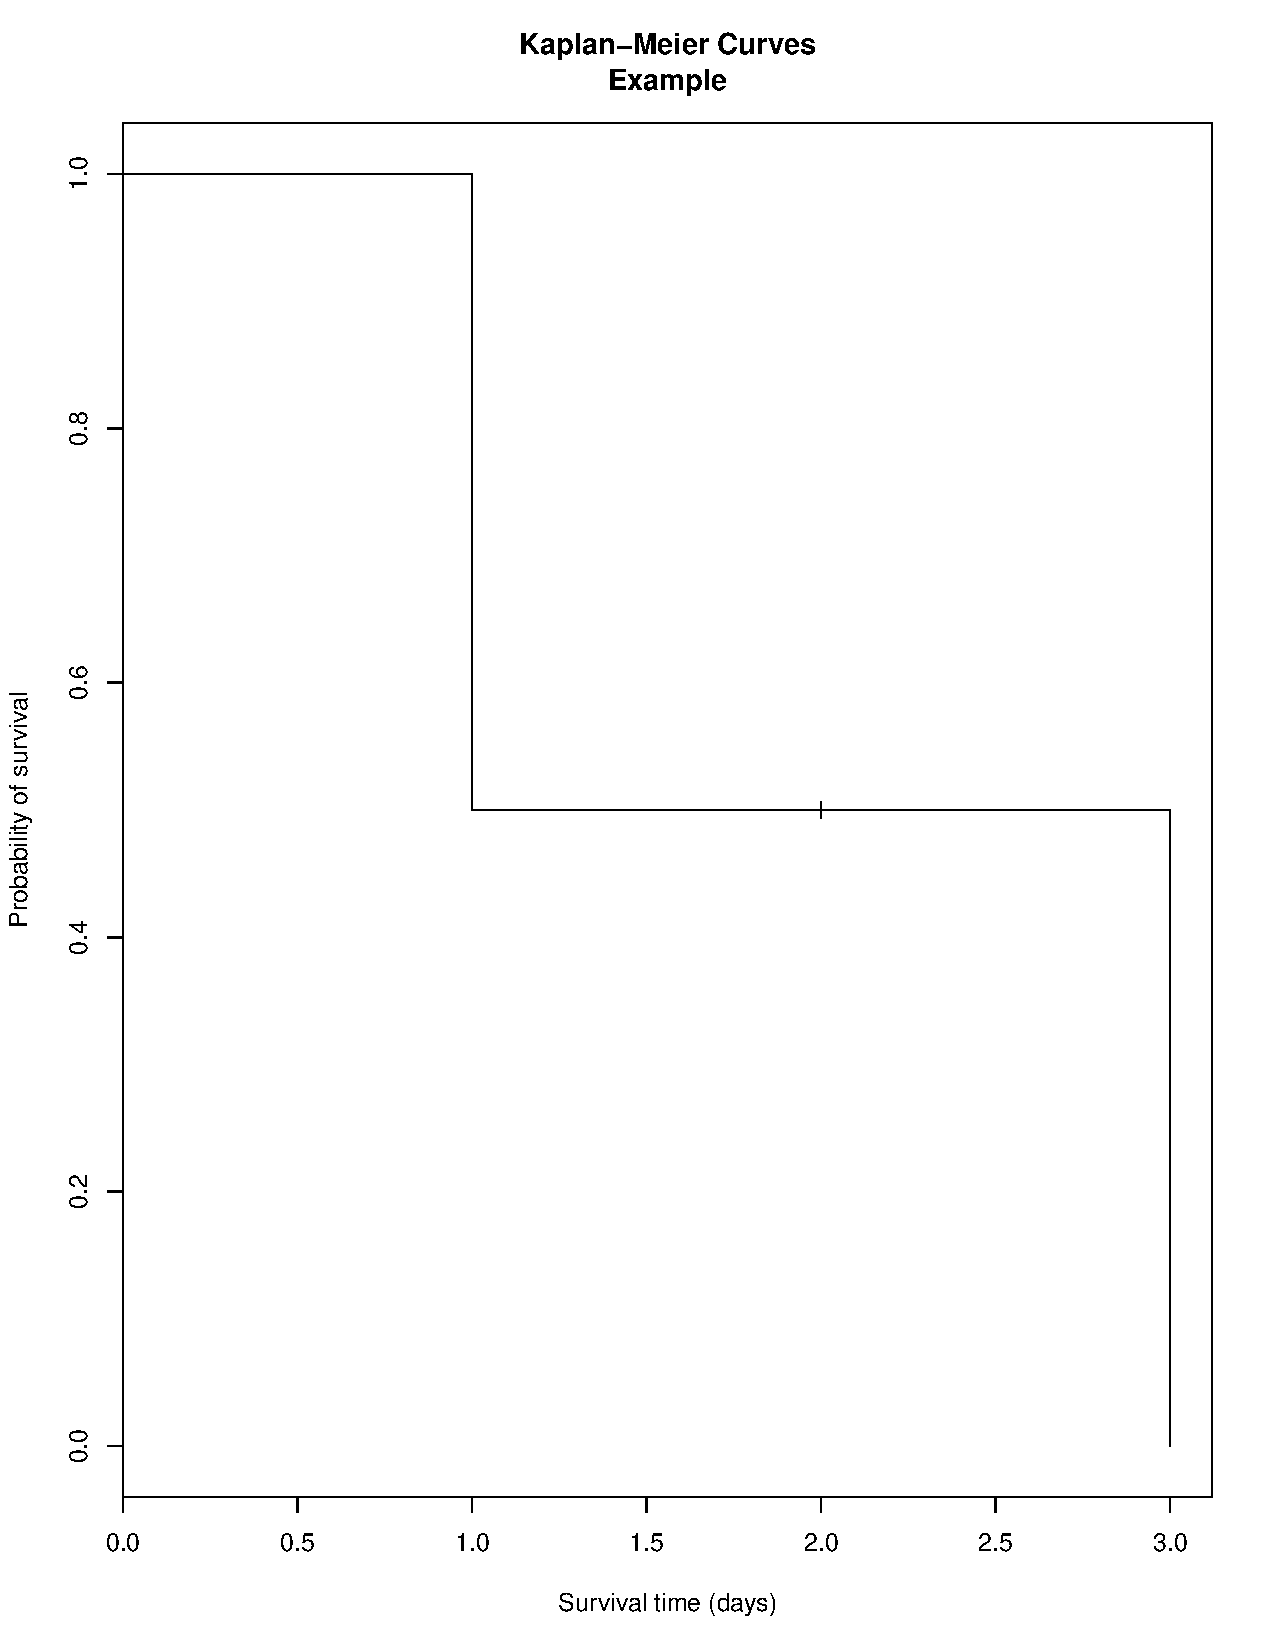
\includegraphics[width=1.0\linewidth]{images/example_survival.pdf}
\caption[Example of survival curve.]{
Example of survival curve for table \ref{survival-example}. Censored data is marked (+) in the plot.}
\end{figure*}



%In analyzing survival data, two functions that are dependent
%on time are of particular interest: the survival function and the
%hazard function.
%The survival function S(t) is defined as the
%probability of surviving at least to time t. The hazard function
%h(t) is the conditional probability of dying at time t having
%survived to that time.

\subsubsection{Comparing survival curves of two groups using the log rank test}

 To compare the survival distributions of two or more groups,  the hypothesis test log-rank test is
 used to test the null hypothesis that there is no difference between the populations
 in the probability of an event at any time point.
%
 The approximated statistics used for comparison purposes for $k$ groups is
 $$T = \sum_{i \in \{1,\ldots,k\}}\frac{(O_i - E_i)^2}{E_i},$$
 where $O_i$ is the observed numbers of death in  group $i$
 while $E_i$ is its expected numbers of deaths.
 If the null hypothesis is true, $T$ is distributed approximately as a $\chi^2_{k-1}$ \cite{matthews1996using}.
If T calculated is $9.44$, and $k = 2$,  evaluating the quantile function (also known as “inverse CDF” or “ICDF”) of the chi-squared distribution the significance level of these data is equal to
$P_r(\chi^2_{1}\geq9.44 = 0.002)$ \cite{yau2012r}.
For a given cut-off, normally $0.05$, the results with p-value smaller are considered significant.

\subsection{Machine Learning}

Machine learning is a field of computer science focused on the development and application of algorithms that improve with experience \cite{mitchell1997machine}.

In genetics and genomics, its  has been applied
 for the interpretation of large genomic data sets and annotation of a wide variety of genomic sequence elements.
For example, for the detection of  transcription start sites (TSSs) locations, which have proven hard to detect in silico due to the complexity and the fairly diffuse structures of Eukaryotic promoters, \citeonline{down2002computational} developped a machine-learning method is able to build useful models of promoters for $>50\%$ of human transcription start sites \cite{down2002computational}.

The machine learning techniques can classified into two main categories: supervised and unsupervised learning (Mitchell, 1997). The supervised learning, which aims to infer data labels by learning from already labeled data, has three stages: design, model and test. The first stage refers to the selection of a learning algorithm used to learn from data (e.g. choose between support vector machines or random forest algoritms) and its training data. The second stage is the creation of a model from labeled data using the algorithm selected priviously.  The last stage uses of this generated model to  preditct the labels of unlabeled data.
The unsupervised learning methods, on the other hand,
cluster the data without using labels, which requires an additional step in which semantics must be manually assigned to each cluster. As this discovery is not tied to previously defined classes, these methods have as benefit the ability to identify potentially novel types of genomic elements.




\subsubsection{Supervised learning}
\subsubsection{Unsupervised learning}



%When a labelled training set is not available, unsupervised learning is required. For example, consider the interpretation of a heterogeneous collection of epigenomic data sets, such as those generated by the Encyclopedia of DNA Elements (ENCODE) Consortium and the Roadmap Epigenomics Project. A priori, we expect that the patterns of chromatin accessibility, histone modifications and transcription factor binding along the genome should be able to provide a detailed picture of the biochemical and functional activity of the genome. We may also expect that these activities could be accurately summarized using a fairly small set of labels. If we are interested in discovering what types of label best explain the data, rather than imposing
%a pre-determined set of labels on the data, then we must use unsupervised rather than supervised learning. In this type of approach, the machine learning algorithm uses only the unlabelled data and the desired number of different labels to assign as input.

% In Transcriptomics analysis clustering is used to build groups of genes with related expression patterns

Unsupervised learning is a type of machine learning algorithm used to draw inferences from datasets consisting of input data without labeled responses.
The most common unsupervised learning method is cluster analysis, which is used for exploratory data analysis to find hidden patterns or grouping in data. These algorithms seeks to group a set of objects into cluster (groups) such that those in the same group are more similar to each other than to those in other cluster.
The major unsupervised learning techniques used in bioinformatics are described below.
%In genomics, the Hierarchical clustering, Centroid-based clustering and PCA are commonly used.
\begin{description}

\item[Hierarchical clustering:] {This clustering methods builds a hierarchy of clusters, through either a agglomerative ("bottom up") or a divisive ("top down") procedures.
In the agglomerative procedures, each $n$ observation starts in its own cluster and until only one cluster remains the groups with the smallest dissimilarity are merged.
On the other hand, in the divise procedures, all observations start in one cluster and until all observations are in their own cluster the group is splitted in two groups with biggest dissimilarity. To decide which clusters to merge or divide a metric to measure of dissimilarity between sets of observations is required.
Among the existing agglomerative techniques are the single linkage, also known as the nearest-neighbour technique, which defines the smallest dissimilarity between two points in each group as the dissimilarity between two groups \cite{florek1951liaison}, the complete linkage which defines the largest dissimilarity between two points in each group as the dissimilarity between two groups \cite{defays1977efficient}, the average linkage which defines the average dissimilarity over all points as the dissimilarity between two groups \cite{sokal1958statistical} and the Ward’s method which at each merge step minimizes the increase in the total within-cluster error sum of
squares, which means that  the groups leading to minimum increase in total within-cluster variance are merged \cite{ward1963hierarchical,everitt2011hierarchical}.
The results of hierarchical clustering are usually represented in a dendrogram a branching diagram in which the objects are represented in one of the axis while the similarity between clusters are represented in the other axis by the length of the connection which joins them \cite{manning1999foundations}.}

\item[Optimization clustering
techniques:]{
These are a set of non-hierarchical clustering techniques that cluster individuals into a specified number of groups, by either minimizing or maximizing some numerical criterion \cite{everitt2011hierarchical}.  One of these technique is the k-means algorithms, which iteratively updates a partition by simultaneously relocating each object to the group to whose mean it was closest and then recalculating the group means until the groups no longer change.
More explicitly, let $S = \{S_1,S_2,\ldots,S_k\}$  be the set of k clusters, this algorithms tries to minimize the squared distances of the elements from the cluster center:
$$ N(n,k) = min\sum_{g = 1}^{k}\sum_{j \in S_g}\Vert x_j - \mu_g\Vert^2,$$
where $x_j$ is a data element that belongs to a group g, and $\mu_g$ is the center of points of the $g$ group. A counterpoint of these techniques also requirement to ‘estimate’ the number of clusters in the data, for which a variety of methods
have been suggested and  most are
relatively informal and involve, essentially, plotting the value of the clustering
criterion against the number of groups in which large changes of levels in the plot are
usually taken as suggestive of a particular number of groups.
Some formal methods were also proposed such as the Silhouette index by \citeonline{rousseeuw1987silhouettes}.
And a second counterpoint of this technique is the choice of initial starting values which might lead to local optimal solution, some solution to this problem such as a  bootstrap-like approach to ‘refine’ initial seeds are suggested \cite{steinley2003local}.
}
\item[Principal component analysis (PCA):]{

PCA is a method for transforming the variables in a multivariate data set into new variables, a linear combination of the original variables, which are uncorrelated with each other and a linear combination of the original variables. This technique provides a means of
projecting the data into a lower dimensional space, which is very useful  mainly due to the problems of high dimensional data which is called ``curse of dimensionality''.
Generally, \citeonline{verleysen2005curse} defines the curse of dimensionality as the expression of all phenomena that appear with high-dimensional data, and that have most often unfortunate consequences on the behavior and performances of learning algorithms. In summary,  the number of learning data should grow exponentially with
the dimension, that means if 10 data  is reasonable to learn a 1-dimensional model, for a 2-dimensional model it will be need 100 data). For example, in genetics, microarray experiments have information for thousand of genes, if each one is considered a variable we would have thousand dimensions,
and we would need an enormous amount of observations to obtain a reliable result. If a dimensionality reduction is not performed, with a increase of data features (dimensions), it is very likely that, by chance, one feature perfectly separates the training examples into positive and negative classes, which would leadto good performance on the training data but poor generalization to data that were not used in training \cite{libbrecht2015machine}.
}
\end{description}

%Another classical and very useful example of unsupervised techniques is the Principal Component Analysis (PCA)


\chapter{Development of methods and softwares for cancer data analysis}
\label{chapter:softwares}

\section{Sotwares developed}

\section{ELMER}

Motivated by our discovery of transcriptional enhancers in tissue DNA methylation data \cite{berman2012ng}, and subsequent approaches to linking these enhancers to transcriptional targets using a chromQTL approach \cite{aran2013dna} (reviewed in \cite{yao2015review}), we developed the the R/Bioconductor  \textit{ELMER} (Enhancer Linking by Methylation/Expression Relationships) package, a tool which infers regulatory element landscapes and transcription factor networks from cancer methylomes \cite{yao2015inferring}. 

This tool combined DNA methylation and gene expression data from human tissues to infer multi-level cis-regulatory networks through several steps which included the identification of distal enhancer probes with significantly altered DNA methylation levels in primary tumor tissues compared to normal tissues, followed by the identification of putative target genes, and a comprehensive gene regulatory network analysis which combined transcription factor motifs at the altered enhancers with TF expression to identify the underlying master regulators. This approach identified several known and unknown master regulators in TCGA data, such as GATA3 and FOXA1 in breast cancer, and P63 and SOX2 in squamous cell lung carcinoma \cite{yao2015inferring,silva2016tcga}.

% Present \textit{ELMER}
Based on user feedback and a full review of the source code, we identified and implemented a number of software improvements, which are summarized in table \ref{tab:summary}: (i) The original package contained no standard data structure to handle multiple assays (DNA methylation, gene expression, and clinical data), which would be required for an integrative genomic data analysis. Recently, the Bioconductor team provided such a data structure through the \href{http://bioconductor.org/packages/MultiAssayExperiment/}{MultiAssayExperiment} package. (ii) All auxiliary databases (human TF list, classification of TF in families, gene annotation, DNA methylation annotation and motif occurrences within probe sites) used in the package were created and maintained manually, thereby making the upgrade process laborious; thus, we automated this process. (iii) The package was developed to analyze primary tumor tissue samples compared to normal tissues samples, thus not allowing arbitrary subgroups to be compared (for instance mutants vs. non-mutants, treated vs. untreated, etc.) (iv) Our original approach used known epigenomic markers for enhancers to constrain the genomic regions searched for differential methylation. However, this selection could limit our algorithm to identifying regulatory networks for tissue types that exist in the epigenomic databases; we found this constraint problematic, and thus now search \textit{all} distal regulatory regions without any such filter. (v) The function used to download data from The Cancer Genome Atlas (TCGA) data portal \cite{tomczak2015cancer} broke when the TCGA site was shutdown and its data transferred to The NCI's Genomic Data Commons (GDC) \cite{grossman2016toward}; we now have a more general data provider interface that supports GDC as the default provider. (vi) The package only supported data aligned to Genome Reference Consortium GRCh37 (hg19), and we now provide support for Genome Reference Consortium GRCh38 (hg38). (vii) There was no support to the recent HumanMethylationEPIC (EPIC) array \cite{epic}. In addition to the specific improvements listed above, we substantially re-wrote most of the code to be more efficient and maintainable,  also most of the output plots generated were improved.

\begin{table}[h!]
\centering
\caption{Main differences between ELMER old version (v.1) and the new version (v.2)}
\label{tab:summary}
\begin{tabular}{@{}p{3cm}p{5cm}p{6cm}@{}}
\toprule
\multicolumn{1}{c}{\textbf{Features}} & \multicolumn{1}{c}{\textbf{ELMER Version 1}} & \multicolumn{1}{c}{\textbf{ELMER Version 2}}   \\ \midrule
Primary data structure                   & mee object (custom data structure)                       & MAE object (Bioconductor data structure) \\
Auxiliary data                   & Manually created                       & Programmatically created \\
Number of human TFs                    & 1,982                                  & 1,987 (Uniprot database \cite{apweiler2004uniprot})                 \\
Number of TF motifs                   & 91                                     & 771  (HOCOMOCO v11 database \cite{kulakovskiy2016hocomoco})                 \\
TF classification                     & 78 families                            & 82 families and 331 subfamilies \newline(TFClass database \cite{wingender2013tfclass}) \\
Analysis performed            & Normal vs tumor samples & Group 1 vs group 2                       \\ 
Statistical grouping            & unsupervised only & unsupervised or supervised using labeled groups                       \\ 
TCGA data source                   & The Cancer Genome Atlas (TCGA) (not available)                   & The NCI's Genomic Data Commons (GDC)                                      \\
Genome of reference                   & GRCh37 (hg19)                          & GRCh37 (hg19)/GRCh38 (hg38)          \\
DNA methylation platforms             & HumanMethylation450                                   & HumanMethylationEPIC and HumanMethylation450                                \\
Graphical User interface (GUI)        & None                                   & TCGAbiolinksGUI                       \\
\bottomrule
\end{tabular}
\end{table}

Here, we present a new version of the R \textit{ELMER} package, which addresses all the issues described above. 
The new version of \textit{ELMER} (v2.0.0) is available as an R/Bioconductor package at \url{https://github.com/tiagochst/ELMER}. And, the new version of \textit{ELMER.data} (v2.0.0), which provides auxiliary data required to perform the analysis, is available at 
\url{https://github.com/tiagochst/ELMER.data}. 

\subsection*{Implementation}
% * <benbfly@gmail.com> 2017-06-09T18:49:35.529Z:
% 
% > Implementation
% Present and past tense are intermixed somewhat in this section.  I think we should use present tense for all methods descriptions, and only use past tense when we are describing a specific analysis run.
% 
% ^.
% For software tool papers, this section should address how the tool works and any relevant technical details required for implementation of the tool by other developers.  
Here we describe each of following analysis steps shown in figure \ref{fig:elmerworkflow}. For more details, please also check the original ELMER paper \cite{yao2015inferring}. 
\begin{itemize}
    \item Organize data as a \textit{MultiAssayExperiment} object
	\item Identify distal probes with significantly different DNA methylation level when comparing two sample groups.
	\item Identify putative target genes for differentially methylated distal probes, using methylation vs. expression correlation
	\item Identify enriched motifs for each probe belonging to a significant probe-gene pair
	\item Identify master regulatory Transcription Factors (TF) whose expression associate with DNA methylation changes at multiple regulatory regions.
\end{itemize}

Organization of data as a \textit{MultiAssayExperiment} object

To facilitate the analysis of experiments and studies with multiple samples the Bioconductor team created the \href{http://bioconductor.org/packages/SummarizedExperiment/}{\textit{SummarizedExperiment}} class \cite{huber2015orchestrating}, a data structure able to store data and metadata for a single experiment but not for data spanning several experiments for the same sample. To overcome this problem, recently, the MultiAssay SIG (Special Interest Group) created the \href{http://bioconductor.org/packages/MultiAssayExperiment/}{MultiAssayExperiment class} \cite{mae2017} a data structure to manage and preprocess multiple assays for integrated genomic analysis. This data structure is now an input for all main functions of \href{https://github.com/tiagochst/ELMER}{\textit{ELMER}} and can be generated by the \textit{createMAE} function. 

%In cancer research, integrative analysis of different molecular data associated with clinical outcome can be used to identify new subgroups of patients, which also might lead to specific improved therapy for this subset of patients \cite{kristensen2014principles}.
%With this trend of integrative analysis, the Bioconductor environment sought to provide a data structure that could integrate this data in the best possible way. One of those integrative data structures created was the \href{http://bioconductor.org/packages/SummarizedExperiment/}{\textit{SummarizedExperiment} container}, which was able to store several arrays if they have an equivalent number of rows and columns \cite{huber2015orchestrating}.


To perform \textit{ELMER} analyses, we need to populate a \textit{MultiAssayExperiment} with a DNA methylation matrix or \textit{SummarizedExperiment} object from HM450K or EPIC platform; a gene expression matrix or SummarizedExperiment object for the same samples; a matrix mapping DNA methylation samples to gene expression samples; and a matrix with sample metadata (i.e. clinical data, molecular subtype, etc.). If TCGA data are used, the last two matrices will be automatically generated.
If using non-TCGA data,  the matrix with sample metadata should be provided with at least a column with a patient identifier and another one identifying its group which will be used for analysis, if samples in the methylation and expression matrices are not ordered and with same names, a matrix mapping for each patient identifier their DNA methylation samples and their gene expression samples should be provided to the \textit{createMAE} function.
Based on the genome of reference selected, metadata for the DNA methylation probes, such as genomic coordinates, will be added from   \href{http://zwdzwd.github.io/InfiniumAnnotation}{\citeonline{zhou2016comprehensive}}; 
and metadata for gene expression and annotation is added from Ensembl database \cite{yates2015ensembl} using \href{http://bioconductor.org/packages/biomaRt/}{biomaRt}
\cite{durinck2009mapping}. 
% * <benbfly@gmail.com> 2017-06-08T12:50:39.539Z:
% 
% > the methylation and expression matrices of the {MultiAssayExperiment} can be populated using the \textit{XXXXXX} function
% @tiago can you fill this in?
% 
% ^ <tiagochst@gmail.com> 2017-06-09T21:44:31.369Z:
% 
% I'll try to rewrite this, actually the function is the same for TCGA and non-TCGA data, but the user will need to a the matrix mapping the samples to groups and another one to map gene expression to dna methylation columns if they don't have the same name. Also, gene expression rows needs to be ensembl gene id (ENSG).
%
% ^.

\subsubsection*{Selecting distal probes} 
Probes from HumanMethylationEPIC (EPIC) array and Infinium HumanMethylation450 (HM450) array are removed from the analysis if they have either internal SNPs close to the $3'$ end of the probe; non-unique mapping to the bisulfite-converted genome; or off-target hybridization due to partial overlap with non-unique elements \cite{doi:10.1093/nar/gkw967}. This probe metadata information is
included in \href{https://github.com/tiagochst/ELMER.data}{\textit{ELMER.data}} package, populated from the source file at \url{http://zwdzwd.github.io/InfiniumAnnotation} \cite{doi:10.1093/nar/gkw967}.
To limit ELMER to the analysis of distal elements, probes located in regions of $\pm2 kb$ around transcription start sites (TSSs) were removed.
% * <tiagochst@gmail.com> 2017-05-19T00:38:48.290Z:
% 
% > distal elements (not in promoter regions),
% Can we say this?
% 
% ^ <benbfly@gmail.com> 2017-06-08T12:55:23.253Z.

\subsubsection*{Identification of differentially methylated CpGs (DMCs)}

For each distal probe, samples of each group (group 1 and group 2) are ranked by their DNA methylation beta values, those samples in the lower quintile (20\% samples with the lowest methylation levels) of each group are used to identify if the probe is hypomethylated in group 1 compared to group 2, using an unpaired one-tailed t-test. The 20\% is a parameter to the \textit{diff.meth} function called \textit{minSubgroupFrac}. For the (ungrouped) cancer case, this is set to 20\% as in \citeonline{yao2015inferring}, because we typically wanted to be able to detect a specific molecular subtype among the tumor samples; these subtypes often make up only a minority of samples, and 20\% was chosen as a lower bound for the purposes of statistical power (high enough sample numbers to yield t-test p-values that could overcome multiple hypothesis corrections, yet low enough to be able to capture changes in individual molecular subtypes occurring in 20\% or more of the cases.) This number can be set arbitrarily as an input to the \textit{diff.meth} function and should be tuned based on sample sizes in individual studies. In the \textit{Supervised} mode, where the comparison groups are implicit in the sample set and labeled, the \textit{minSubgroupFrac} parameter is set to 100\%.  An example would be a cell culture experiment with 5 replicates of the untreated cell line, and another 5 replicates that include an experimental treatment.
% * <benbfly@gmail.com> 2017-06-08T13:32:21.874Z:
% 
% >  In the \textit{Supervised} mode
% I really would like to have a Supervised version of the pipeline where the percentage is not set at all, but automatically defaults to 100% .  This would be used for two group replicate comparisons like the one I describe.
% 
% ^ <tiagochst@gmail.com> 2017-06-09T21:47:56.390Z:
% 
% The pipeline you mean the TCGA_pipe function, which does all the code? We can remove percentage argument from it and add one "mode" supervised (all samples) unsupervised 20%. 
%
% ^ <tiagochst@gmail.com> 2017-06-09T23:50:55.816Z.
% * <benbfly@gmail.com> 2017-06-08T13:32:04.138Z:
% 
% > minSubgroupFrac
% What is the actual name of this parameter?  It should be named something intuitive since it is really important
% 
% ^ <tiagochst@gmail.com> 2017-06-09T21:48:57.068Z:
% 
% It was percentage in all functions. I'll see what I can do
%
% ^ <tiagochst@gmail.com> 2017-06-09T23:50:45.422Z:
% 
% I changed to minSubgroupFrac in the code
%
% ^ <tiagochst@gmail.com> 2017-06-09T23:50:51.139Z.

To identify hypomethylated DMCs, a one-tailed t-test is used to rule out the null hypothesis: $\mu_{group1} \geq \mu_{group2}$, where $\mu_{group1}$ is the mean methylation within the lowest group 1 quintile (or another percentile as specified by the \textit{minSubgroupFrac} parameter) and $\mu_{group2}$ is the mean within the lowest group 2 quintile. Raw p-values are adjusted for multiple hypothesis testing using the Benjamini-Hochberg method \cite{benjamini1995controlling}, and probes are selected when they had adjusted p-value less than $0.01$ (which can be configured using the \textit{pvalue} parameter). For additional stringency, probes are only selected if the methylation difference: $\Delta = \mu_{group1} - \mu_{group2}$ was greater than $0.3$. The same method is used to identify hypermethylated DMCs, except we use the \textit{upper} quintile, and the opposite tail in the t-test is chosen.
% * <benbfly@gmail.com> 2017-06-09T18:19:56.660Z:
% 
% > minDMCpval
% change this to the actual name
% 
% ^ <tiagochst@gmail.com> 2017-06-09T23:51:02.993Z.

\subsubsection*{Identification of putative target gene(s)} 

For each differentially methylated distal probe (DMC), the closest 10 upstream 
genes and the closest 10 downstream genes are tested for inverse correlation between 
methylation of the probe and expression of the gene (the number 10 can be changed using the \textit{numFlankingGenes} parameter). To select these genes, 
% * <benbfly@gmail.com> 2017-06-09T18:27:35.572Z:
% 
% > numFlankingGenes
% Does this parameter actually exist?  It should .. 
% 
% ^ <tiagochst@gmail.com> 2017-06-09T21:53:14.901Z:
% 
% I maintained Lijing's approach, we have a external function (https://github.com/tiagochst/ELMER/blob/master/R/GetNearbyGenes.R#L171-L176) . But I can change this and add to the get.pair and just add this numFlanking genes parameter.
%
% ^ <tiagochst@gmail.com> 2017-06-09T23:39:50.202Z:
% 
% I decided to keep the function outside. But I change the argument to numFlankingGenes instead of geneNum
%
% ^ <tiagochst@gmail.com> 2017-06-09T23:51:07.261Z.
the probe-gene distance is defined as the distance from the probe to the transcription 
start site specified by the ENSEMBL gene level annotations \cite{yates2015ensembl} accessed via
the R/Bioconductor package \href{http://bioconductor.org/packages/biomaRt/}{biomaRt} \cite{durinck2009mapping,durinck2005biomart}. By choosing a constant number of genes to test for each probe, our goal is to avoid systematic false positives for probes in gene rich regions. This is especially important given the highly non-uniform gene density of mammalian genomes.
Thus, exactly 20 statistical tests were performed for each probe, as follows. 

For each probe-gene pair, the samples (all samples from both groups) are divided into two 
groups: the M group, which consisted of the upper methylation quintile (the 20\%
of samples with the highest methylation at the enhancer probe), and the U group, 
which consists of the lowest methylation quintile (the 20\% of samples with the 
lowest methylation.) The 20\% ile cutoff is a configurable parameter \textit{minSubgroupFrac} in the \textit{get.pair} function.
As with its usage in the \textit{diff.meth} function, the default value of 20\% is a balance, allowing for the identification of changes in a 
molecular subtype making up a minority (i.e. 20\%) of cases, while also yielding 
enough statistical power to make strong predictions. For larger sample sizes or other experimental designs, this could be set even lower.

For each candidate probe-gene pair, 
the Mann-Whitney U test is used to test the null hypothesis that overall gene 
expression in group M is greater than or equal than that in group U. 
This non-parametric test was used in order to minimize the effects 
of expression outliers, which can  occur across a very wide dynamic range. 
For each probe-gene pair tested, the raw p-value $P_r$ is corrected for multiple 
hypothesis using a permutation approach as follows.
The gene in the pair is held constant, and \textit{x} random methylation probes are 
chosen to perform the same one-tailed U test, generating a set of \textit{x} permutation
p-values $P_p$. We chose the x random probes only from among those that were 
"distal" (farther than $2kb$ from an annotated transcription start site), in order 
to draw these null-model probes from the same set as the probe being tested \cite{sham2014statistical}. 
An empirical p-value $P_e$ value was calculated using the following formula 
(which introduces a pseudo-count of 1):

$$P_e = \frac{num(P_p \leq P_r)+ 1}{x+1}$$

Notice that in the \textit{Supervised} mode, no additional filtering is necessary to ensure that the M and U group segregate by sample group labels.  The two sample groups are segregated by definition, since these probes were selected for their differential methylation, with the same directionality, between the two groups. 



\subsubsection*{Characterization of chromatin state context of enriched probes using FunciVar}

Unlike version 1 of \textit{ELMER}, we now consider \textit{all} distal probes in the identification of regulatory elements. DNA methylation is known to affect several different classes of distal chromatin state element, including active enhancers, poised enhancers, and insulators. In order to provide a functional interpretation of the regulatory elements identified by \textit{ELMER}, we perform a chromatin state enrichment analysis of the probes within significant probe-gene pairs, using the \textit{statePaintR} tools from the \url{statehub.org} \cite{statepaintr}, along with our new FunciVar package \cite{funcivar}. Enrichment of the putative pairs within chromatin states is calculated against a background model that uses the distal probe set that the putative pairs are drawn from. 

\subsubsection*{Motif enrichment analysis}

In order to identify enriched motifs and potential upstream regulatory TFs, all probes with occurring in significant probe-gene pairs are combined for motif enrichment analysis. \sigla{HOMER}{Hypergeometric Optimization of Motif EnRichment} \cite{heinz2010simple} is used to find motif occurrences in a $\pm 250bp$ region around each probe, using \sigla{HOCOMOCO}{HOmo sapiens COmprehensive MOdel COllection} v11 \cite{kulakovskiy2016hocomoco} . Transcription factor (TF) binding models are available at \url{http://hocomoco.autosome.ru/downloads} (using the HOMER specific format with threshold score levels corresponding to p-value $ \leq 1^{-4}$). 

For each probe set tested (i.e. the set of all probes occurring in significant probe-gene pairs), a motif enrichment Odds Ratio and a 95\% confidence interval are calculated using following formulas:
$$p = \frac{a}{a + b}$$
$$P = \frac{c}{c + d}$$
$$Odds Ration = \frac{\frac{p}{(1-p)}}{\frac{P}{1-P}}= \frac{p(1-P)}{P(1-p)}=\frac{ad}{bc}$$
$$SD = \sqrt{\frac{1}{a} + \frac{1}{b} + \frac{1}{c} + \frac{1}{d}}$$

where $a$ is the number of probes within the selected probe set that contains one 
or more motif occurrences; $b$ is the number of probes within the selected probe 
set that do not contain a motif occurrence; $c$ and $d$ are the same counts within 
the entire array probe set (drawn from the same set of distal-only probes using the same definition as the primary analysis). A probe set was considered significantly enriched 
for a particular motif if the 95\% confidence interval of the Odds Ratio was 
greater than $1.1$ (specified by option \textit{lower.OR}, $1.1$ is default), and the motif 
occurred at least 10 times (specified by option \textit{min.incidence}, $10$ is default) in 
the probe set. 

%\section*{Results} % Optional - only if novel data or analyses are included
%This section is only required if the paper includes novel data or analyses, and should be written as a traditional results section.

\subsubsection*{Identification of master regulator TFs}

When a group of enhancers is coordinately altered in a specific sample subset, this is often the result of an altered upstream \textit{master regulator} transcription factor in the gene regulatory network. \textit{ELMER} tries to identify such transcription factors corresponding to each of the TF binding motifs enriched from the previous analysis step.
For each enriched motif, \textit{ELMER} takes the average DNA methylation of all distal probes (in significant probe-gene pairs) that contain that motif occurrence (within a $\pm 250bp$ region) and compares this average DNA methylation to the expression of each gene annotated as a human TF.

A statistical test is performed for each motif-TF pair, as follows. All samples 
are divided into two groups: the M group, which consists 
of the 20\% of samples with the highest average methylation at all motif-adjacent
probes, and the U group, which consisted of the 20\%  of samples with the lowest 
methylation. This step is performed by the \textit{get.TFs} function, which takes \textit{minSubgroupFrac} as an input parameter, again with a default of 20\%.
For each candidate motif-TF pair, the Mann-Whitney U test is used to test 
the null hypothesis that overall gene expression in group M is greater or equal 
than that in group U. This non-parametric test was used in order to minimize the 
effects of expression outliers, which can occur across a very wide dynamic range. 
For each motif tested, this results in a raw p-value ($P_r$) for each of the human TFs.
All TFs are ranked by their $-log_{10}(Pr)$ values, and those falling within the top 5\% of 
this ranking were considered candidate upstream regulators. The best upstream 
TFs which are known to recognize to specific binding motif are automatically extracted as putative 
regulatory TFs, and rank ordered plots are created to visually inspect these relationships, as shown in the example below. Because the same motif can be recognized by many transcription factors of the same binding domain family, we define these relationships at both the family and subfamily classification level using the 
classifications from TFClass database \cite{wingender2013tfclass}. Use of this database is a major change from version 1 of ELMER, which used custom curations for DNA binding domain families. Use of the TFClass database is preferable because it is well curated and regularly updated to reflect new findings.



%\begin{landscape}
\tikzstyle{container} = [
    rectangle,
    draw,
    inner sep=0.2 cm,
    dashed
]
\tikzstyle{start} = [circle,
					 minimum size=2mm,
                     rounded corners=3mm,
					 very thick,
                     draw=green!50!black,
                     top color=green!50!black,
                     bottom color=green!50!black, 
                     text=white,
                     font=\tiny]

\tikzstyle{end} = [circle,
				  minimum size=2mm,
                  rounded corners=3mm,
                  very thick,draw=red!50!black, 
                  top color=red!50!black,
                  bottom color=red!50!black, 
                  text=white,
                  font=\tiny]

\tikzstyle{function} = [rectangle,
						minimum size=6mm,
                        rounded corners=3mm,
                        very thick,
                        draw=black!50, 
                        top color=white,
                        bottom color=white,
                        font=\itshape\footnotesize]

\tikzstyle{datain} = [
	rectangle, 
	rounded corners, 
    minimum width=3cm, 
    minimum height=0.5cm,
    text centered,
    font=\footnotesize, 
    draw=green!50!black, 
    fill=white, 
    text=black
]
                      
\tikzstyle{dataaux} = [
	rectangle, 
    rounded corners, 
    minimum width=3cm, 
    minimum height=0.5cm,
    text centered,
    font=\footnotesize,
    draw=orange, 
    fill=white, 
    text=black
]
                       
\tikzstyle{dataout} = [
	rectangle, 
	rounded corners, 
    minimum width=3cm, 
    minimum height=0.5cm,
    text centered,
    font=\footnotesize, 
    draw=blue, 
    fill=white, 
    text=black
]

% Pacakge labels
\tikzstyle{arrow} = [
	thick,
    ->,
    >=stealth,
    -latex',
    draw,
    rounded corners
]

\tikzstyle{labelelmer}=[
	rectangle,
    draw,
    fill=black!50!red,
    draw = black,
    minimum width=450pt,
    minimum height=1.5em,
    text=white,
    rotate = 90, 
    label={[rotate=90]center:\textcolor{white}{\textbf{ELMER package}}}
]

\tikzstyle{labeltcgabiolinks}=[
	rectangle,
	draw,
    fill=black!50!blue,
    draw = black,
    minimum width=420pt,
    minimum height=1.5em,
    text = green,
    rotate = 90, 
    label={[rotate=270]center:\textcolor{white}{\textbf{TCGAbiolinks/TCGAbiolinksGUI packages}}}
]


\tikzstyle{labelfuncivar}=[
	rectangle,
	draw,
    fill=black!20!orange,
    draw = black,
    xshift = -0.0cm,
    minimum width=480pt,
    minimum height=1.5em,
    text=white,
    rotate = 0, 
    label={[rotate=0]center:\textcolor{white}{\textbf{StateHub/StatePaintR/funcivar package}}}
]
\tikzstyle{labelgdc}=[
	rectangle,
	draw,
    fill=black!50!gray,
    draw = black,
    minimum width=167pt,
    minimum height=1.5em,
    text=white,
    yshift = 0.10cm,
    xshift = 0.1cm,
    rotate = 0, 
    label={[rotate=0]center:\textcolor{white}{\textbf{GDC database}}}
]
\tikzstyle{every annotation}=[fill=white, font=\sf \small, scale=0.5, text width=4cm, inner sep=2mm, text=black,draw = orange]


\begin{figure}[!ht]
\centering
  \resizebox{0.95\textwidth}{!}{%
\begin{tikzpicture}[node distance = 1.5cm, auto, shorten >=1pt,thick,font=\itshape\footnotesize]
\linespread{0.8}{
%\node (start) [start] {START};
\node (func1) [function, yshift = -0.5cm] {\textit{createMAE}};
\node [datain, right of=func1, yshift = 0.5cm, xshift = 2cm] (dna) {DNA methylation object};
\node [datain, right of=func1, yshift = -0.5cm, xshift = 2cm] (exp) {Gene expression object};
\node (out1) [dataout, below of=func1, yshift = -0.3cm,text width=3cm] {Multi Assay Experiment object};
\node (func2) [function, below of = out1] {get.diff.meth};
%\node (out2) [dataout, below of=func2, yshift = 0.3cm] {List of differently methylated probes};
\node (func3) [function, below of=func2] {GetNearGenes};
%\node (out3) [dataout, below of=func2, yshift = 0.3cm] {List of near genes for differently methylated probes};
\node (func4) [function, below of=func3] {get.pair};
%\node (out4) [dataout, below of=func4, yshift = 0.3cm] {List of pairs: differently expressed gene and differently methylated probes};
\node (func5) [function, below of=func4, yshift = -0.5cm] {get.enriched.motif};
%\node (out5) [dataout, below of=func5, yshift = 0.3cm] {List of enriched motifs};
\node (func6) [function, below of=func5] {get.TFs};
\node (func7) [function, below of=func6,yshift = -0.5cm] {TF.survival};
%\node (out5) [dataout, below of=func5, yshift = 0.3cm] {List of regulator};
\node [dataaux, left of=func5, xshift =-3cm] (elmerdata1) {Probes.motif};
%\node [dataaux, above of=elmerdata1] (enhancer) {enhancer};
\node [dataaux, left of=func6, yshift = 0.0cm, xshift =-3cm] (elmerdata2) {motif.relevant.TFs};
\node [dataaux, left of=func6, yshift = -1.0cm, xshift =-3cm] (elmerdata3) {human.TFs};
%\node (end) [end, below of=func7] {END};
\node (func8) [function, left of=func1,yshift = -3cm,xshift = -3cm] {get.feature.probe};
\node (probes) [datain, left of=func1,xshift = -3cm] {distal probes};
\node [dataaux, below of=func8] (tss) {ENSEMBL TSS};
\node [dataaux, below of=tss] (probesmetadata) {Probes metadata};


% funcvat
\node (funciVar) [function, below of=func7, xshift = 3cm, yshift = -1.4cm] {enrich.segments};
\node [dataaux, left of=funciVar,xshift = -2cm] (statehub) {Statehub tracks};
%\node [dataaux, left of=statehub,xshift = -2cm, yshift = 0.2cm] (encode) {ENCODE};
%\node [dataaux, left of=statehub,xshift = -2cm, yshift = -0.4cm] (roadmap) {ROADMAP};
%\node [dataaux, left of=statehub,xshift = -2cm, yshift = 0.8cm] (blueprint) {BLUEPRINT};
%\draw [arrow,dashed,draw=orange] (encode.east) -- (statehub.west);
%\draw [arrow,dashed,draw=orange] (roadmap.east) -- (statehub.west);
%\draw [arrow,dashed,draw=orange] (blueprint.east) -- (statehub.west);

\draw [arrow,dashed,draw=orange] (statehub.east) -- (funciVar.west);

\draw [arrow] (func4) -- ++(4.9,0) -- ++(0,-1) |- node {} (funciVar);

% Draw edges
%\path [arrow] (start) -- (func1);
\path [arrow,dashed,draw=green!50!black] (dna) |- (func1);
\path [arrow,dashed,draw=green!50!black] (exp) |- (func1);
\draw [arrow,dashed,draw=blue] (out1.west) -- ++(-.5,0) -- ++(0,-1) |- (func4.west);
\draw [arrow,dashed,draw=blue] (out1.west) -- ++(-.5,0) -- ++(0,-1) |- (func6.west);
\draw [arrow] (func1) -- (out1);
\draw [arrow] (out1) -- (func2);
\draw [arrow] (func2) -- node {} (func3);
\draw [arrow] (func3) -- (func4);
\draw [arrow] (func4) -- node {} (func5);
\draw [arrow] (func5) -- node {}(func6);
\draw [arrow] (func6) -- (func7);
%\draw [arrow] (func7) -- (end);
\draw [arrow,dashed,draw=orange] (elmerdata1) -- node {} (func5);
\draw [arrow,dashed,draw=orange] (elmerdata2.east) -- (func6.west);
\draw [arrow,dashed,draw=orange] (elmerdata3.east) -- ++(.5,0) -- ++(0,0.2) |- (func6.west);
%\draw [arrow,dashed,draw=orange] (enhancer.north) -- (func8.south);
\draw [arrow,dashed,draw=orange] (tss.north) -- (func8.south);
\draw [arrow,dashed,draw=orange] (probesmetadata.east) -- ++(.1,0) -- ++(0,0.2) |- (func8.east);
\path [arrow,dashed,draw=green!50!black] (probes) -- (func1);
\draw [arrow] (func8.north)  --  (probes);

% Containers
\node [container, 
       fit=(exp)(dna)(func1)(probes), 
       label={[font=\scriptsize,anchor=east] west:Data input}]
       (container1){};
\node [container, 
	   fit=(func2), 
       label={[font=\scriptsize,anchor=west,name=lfunc1] east:{\parbox[c]{4.0cm}{Identifying differentially\\ methylated probes}}}]
       (container2){};
\node [container, 
       fit=(func3)(func4), 
	   label={[font=\scriptsize,anchor=west,name=lfunc2] east:{\parbox[c]{4.0cm}{Identifying putative \\probe-gene pairs}}}]
       (container3){};
\node [container, 
 	   fit=(func5), 
       label={[font=\scriptsize,anchor=west] east:{\parbox[c]{4.0cm}{Motif enrichment\\ analysis}}}]
       (container4){};
\node [container, 
       fit=(func6), 
       label={[font=\scriptsize,anchor=west] south east:Identifying regulatory TFs}]
       (container5){};
\node [container, 
       fit=(elmerdata1)(elmerdata1), 
       label={[name=l1,font=\scriptsize,anchor=east] west:ELMER.data}]
       (container6){};
%\node[draw,text width=3cm, above of = elmerdata1]{ELMER.data};
\node [container, 
	   fit=(func8)(probesmetadata), 
	   label={[name=l3,font=\scriptsize,anchor=east] west:{\parbox[r]{2.0cm}{Select probes \\$\pm 2Kb$  distant \\ from TSS}}}]
       (container8){};

\node [container, 
       fit=(elmerdata2), 
       label={[name=l2,font=\scriptsize,anchor=east] west:TFClass database}]
       (container7){};
\node [container, 
	   fit=(elmerdata3), 
	   label={[name=l3,font=\scriptsize,anchor=east] west:Uniprot database}]
       (container8){};
\node [draw,  
       minimum height=450pt,
	   minimum width=450pt,
       fit=(l1)(exp)(dna)(elmerdata3)(l2)(lfunc1)(lfunc2)]
       (container9){};
\node at (container9.west) [labelelmer] {};
  
%------------------------------ TCGAbiolinks
\node (GDCprepare) [function, right of = func1, yshift =-1.3cm,xshift =8.8cm] {\textit{GDCprepare}};
\node (GDCdownload) [function, above of = GDCprepare,yshift =-0.4cm] {\textit{GDCdownload}};
\node (GDCquery) [function, above of = GDCdownload,yshift =-0.4cm] {\textit{GDCquery}};
\node (TCGAanalysesurvival) [function, right of = func7,xshift =7.8cm] {\textit{TCGAanalyse\_survival}};
\node (TCGAanalyzeEAcomplete) [function, right of = func4,yshift =0.4cm,xshift =7.8cm] {\textit{TCGAanalyze\_EAcomplete}};
\node (TCGAanalyzePathview) [function, right of = func4,yshift =-0.7cm,xshift =7.8cm] {\textit{TCGAanalyze\_Pathview}};
\node (TCGAvisualizeoncoprint) [function, right of = func4,yshift =-1.8cm,xshift =7.8cm] {\textit{TCGAvisualize\_oncoprint}};

\draw [arrow] (GDCquery) -- node {}(GDCdownload);
\draw [arrow] (GDCdownload) -- (GDCprepare);
\draw [arrow] (GDCprepare.west) -- ++(-0.3,0) -- ++(0,0.2) |- (dna.east);
\draw [arrow] (GDCprepare.west) -- ++(-0.3,0) -- ++(0,0.2) |- (exp.east);

\node (subtypeinfo) [dataaux, below of = GDCprepare,yshift =0.6cm] {Subtype information};
\node (molecularinfo) [dataaux, below of = subtypeinfo,yshift =0.6cm] {Molecular data};
\node (clinicalinfo) [dataaux,  below of = molecularinfo,yshift =0.6cm] {Clinical data};
\node (mafinfo) [dataaux, below of = clinicalinfo,yshift =0.6cm] {Mutation data};

\draw [arrow,dashed,draw=orange] (mafinfo.east) -- ++(0.5,0) -- ++(0,-0.2) |-    (TCGAvisualizeoncoprint.east);
\draw [arrow,dashed,draw=orange] (clinicalinfo.east)  -- ++(0.3,0) -- ++(0,0.2) |-   (GDCprepare.east);
\draw [arrow,dashed,draw=orange] (subtypeinfo.east)   -- ++(0.2,0) -- ++(0,0.2) |-   (GDCprepare.east);
\draw [arrow,dashed,draw=orange] (molecularinfo.east) -- ++(0.3,0) -- ++(0,0.2) |-  (GDCprepare.east);
\node [draw,  
       minimum height=420pt,
       minimum width=170pt, 
       xshift = 0.25cm,
       yshift = -0.25cm,
       fit=(TCGAanalyzeEAcomplete)(GDCquery)(TCGAanalysesurvival)(clinicalinfo)(subtypeinfo)](container10){};
\node at (container10.east) [labeltcgabiolinks] {};
\draw [latex'-latex',double] (TCGAanalysesurvival) --  (func7);
\draw [arrow] (func4.east)  -- ++(4.4,0) -- ++(0,0.2) |-  (TCGAanalyzeEAcomplete);
\draw [arrow] (func4.east)  -- ++(4.4,0) -- ++(0,-0.2) |-  (TCGAanalyzePathview);
\draw [arrow] (func4.east)  -- ++(4.4,0) -- ++(0,-0.2) |-  (TCGAvisualizeoncoprint);
\draw [arrow] (func6.east)  -|   (TCGAvisualizeoncoprint.south);
%------------------------------ 
\node [labelgdc, above of = GDCquery,xshift=-0.30cm,yshift=-0.05cm] (gdc) {};
\draw [latex'-latex',double] (GDCquery) --  (gdc.300);

\draw [draw,dashed] (gdc.188) |- (GDCdownload.west);
\draw [arrow,dashed] (gdc.188) |- (mafinfo.west);
\draw [arrow,dashed] (gdc.188) |- (clinicalinfo.west) ;
\draw [arrow,dashed] (gdc.188) |- (molecularinfo.west) ;
}

\tikzstyle{labelencode}=[
	rectangle,
	draw,
    fill=black!50!gray,
    draw = black,
    minimum width=150pt,
    minimum height=1.5em,
    text=white,
    yshift = 0.10cm,
    xshift = 0.1cm,
    rotate = 0, 
    label={[rotate=0]center:\textcolor{white}{\textbf{ENCODE database}}}
]
\tikzstyle{labelroadmap}=[
	rectangle,
	draw,
    fill=black!50!gray,
    draw = black,
    minimum width=150pt,
    minimum height=1.5em,
    text=white,
    yshift = 0.10cm,
    xshift = 0.1cm,
    rotate = 0, 
    label={[rotate=0]center:\textcolor{white}{\textbf{ROADMAP database}}}
]
\tikzstyle{labelblueprint}=[
	rectangle,
	draw,
    fill=black!50!gray,
    draw = black,
    minimum width=150pt,
    minimum height=1.5em,
    text=white,
    yshift = 0.10cm,
    xshift = 0.1cm,
    rotate = 0, 
    label={[rotate=0]center:\textcolor{white}{\textbf{BLUEPRINT database}}}
]

\node [draw,  
       minimum height=6.52em,
       minimum width=480pt, 
       xshift = 1.60cm,
       yshift = 0.05cm,
       fit=(funciVar)(funciVar)](containerFunciVar){};
\node at (containerFunciVar.south) [labelfuncivar] {};


\node [labelencode, right of = statehub,xshift=-8.20cm,yshift=-0.15cm] (encode) {};
\node [labelroadmap, below of = encode,xshift=-0.1cm,yshift=0.7cm] (roadmap) {};
\node [labelblueprint, above of = encode,yshift=-0.8cm,xshift=-0.1cm] (blueprint) {};
%\draw [latex'-latex',double] (encode.180) --  (containerFunciVar.0);
\draw [double,->] (encode.0) --  (statehub.180);
\draw [double,->] (roadmap.0) -- ++(1.4,0) |-   (statehub.180);
\draw [double,->] (blueprint.0) -- ++(1.4,0) |-  (statehub.180);
\end{tikzpicture}
  }%
  
  \caption[ELMER workflow]{ELMER workflow: ELMER receives as input a DNA methylation object, a gene expression object (a matrix or a SummarizedExperiment object) and a Genomic Ranges (GRanges) object with distal probes to be used as filter which can be retrieved using the \textit{get.feature.probe} function. The function \textit{createMAE}  will create a Multi Assay Experiment object keeping only samples that have both DNA methylation and gene expression data. Genes will be mapped to genomic position and annotated using ENSEMBL database \cite{doi:10.1093/database/baw093}, while for probes it will add annotation from \citeauthor{doi:10.1093/nar/gkw967} (\href{http://zwdzwd.github.io/InfiniumAnnotation}{http://zwdzwd.github.io/InfiniumAnnotation}) . This MAE object will be used as input to the next analysis functions. First, it identifies differentially methylated probes followed by the identification of their nearest genes (10 upstream and 10 downstream) through the  \textit{get.diff.meth} and  \textit{GetNearGenes} functions respectively. For each probe, it will verify if any of the nearby genes were affected by its change in the DNA methylation level and a list of  gene and probes pairs will be outputted from \textit{get.pair} function. For the probes in those pairs, it will search for enriched regulatory Transcription Factors motifs with the  \textit{get.enriched.motif} function. Finally, the  enriched motifs will be correlated with the level of the transcription factor through the \textit{get.TFs} function. In the figure green Boxes represents user input data, blue boxes represents output object, orange boxes represent auxiliary pre-computed data and gray boxes are functions.}
  \label{fig:elmerworkflow}
\end{figure}
%\end{landscape}


\chapter{Cancer data analysis}

This chapter presents results of the analysis of cancer data using the
software and algorithms presented in the previous chapter. In section
\ref{sec:analysis_tcgbiolinks} we present some use cases using mainly the TCGAbiolinks
package. In section \ref{sec:analysis_elmer} we present some data analysis using the ELMER package.
In section \ref{sec:glioma_analysis}, using the previous tools described we perfom a
glioma analysis focused specially in the two molecular subtypes G-CIMP-low and
 G-CIMP-high discovered by our laboratory and collaborators.

\section{Use cases using TCGAbiolinks}\label{sec:analysis_tcgbiolinks}

In this section, we introduce and describe the utility and application of TCGAbiolinks
through some use cases.
In subsection  \ref{subsec:analysis_tcgbiolinks2} we show a
lower-grade glioma downstream analysis with gene expression.
In subsection \ref{subsec:analysis_tcgbiolinks3} we show a
downstream analysis integration of gene expression and methylation data of colon
adenocarcinoma data, describing how to generate a starburst plot \cite{noushmehr2010identification},
which was introduced to illustrate the results of integrating
DNA methylation and gene expression data.


\subsection{Lower-grade glioma downstream analysis with gene expression} \label{subsec:analysis_tcgbiolinks2}

For this case study, we used the recently available \sigla{LGG}{lower-grade glioma} data to investigate gene expression differences between the reported molecular subtypes (IDHmutant, IDHwildtype and IDHmutant codels) \cite{platforms2015comprehensive}. In particular, we used TCGAbiolinks to download 293 samples profiled using messenger RNA expression (IlluminaHiSeq RNASeqV2) with available molecular subtypes. The data was normalized using the \textit{TCGAanalyze\_Normalization} function and we applied three filters to remove features/mRNAs with low signals across samples, obtaining 4578, 4284 and 1187 mRNAs, respectively. A clustering analysis was then applied using the ConsensusClusterPlus package \cite{wilkerson2010consensusclusterplus} which identified four distinct groups of samples (EC1-EC4) (Figure \ref{fig:caseexp}A). The survival curves for each cluster were generated using \textit{TCGAanalyze\_survival} and are shown in Figure \ref{fig:caseexp}B. As expected, each cluster effectively separated IDHwildtype tumors (EC1) from IDHmutant-non-codel (EC2) and IDHmutant-codel tumors (EC3 and EC4) (Figure \ref{fig:caseexp}). Additional biological subtypes (DNA methylation subtypes) were reproduced as expected (Figure \ref{fig:caseexp}D) \cite{platforms2015comprehensive}.

\begin{figure*}
\centering
%\includegraphics[width=.9\linewidth]{figures/case3_improved.pdf}
\includegraphics[width=1.0\linewidth]{images/figure4.pdf}
\caption[Case study - LGG downstream analysis with gene expression]{Case study - Integrative (or Downstream) analysis of gene expression and clinical data from LGG disease with unsupervised clustering and crossing expression clusters with clinical and molecular information. \textbf{(A)} Heatmap of 1187 more variables genes clustered with tree $k = 4$ in EC1, EC2, EC3, EC4. \textbf{(B)} Kaplan Meier survivals plot for EC clusters. \textbf{(C and D)} Distribution of the DNA Methylation clusters and ATRX mutation within the EC clusters.}
\label{fig:caseexp}
\end{figure*}

\subsection{Downstream analysis integration of gene expression and methylation data} \label{subsec:analysis_tcgbiolinks3}

The DNA methylation of specific promoter CpG islands has the potential to influence gene expression.
In this case study, we used TCGAbiolinks to examine the biological relationship between DNA methylation
and gene expression in \sigla{COAD}{Colon adenocarcinoma}. Using \textit{GDCquery}, \textit{GDCdownload}
and \textit{GDCprepare}, we obtained DNA methylation data (Infinium HumanMethylation450 and Infinium
HumanMethylation27 platforms) and gene expression data (IlluminaGA RNASeqV2 platform) for the same
TCGA COAD samples \cite{cancer2012comprehensive}. A supervised analysis was performed on the molecular
subtypes CIMP-Low [CIMP.L] and CIMP-High [CIMP.H].
The gene expression analysis started by the identification of outliers, followed by the normalization methods.
 Using \textit{TCGAanalyze\_DEA}, 34 DEGs ($log_2FC\geq 3.0$ and FDR $\leq 10^{-4}$) were identified.
 The result of this analysis is represented in a volcano plot (Figure \ref{fig:case_starburst}A)
 created using \textit{TCGAVisualize\_volcano}.
For the DNA methylation analysis,
using \textit{TCGAanlayze\_DMR} we identified 73 CpG-methylated probes ($\Delta\overline{\beta}\geq 0.25$ and  $FDR \leq 10^{-5}$;  (Figure \ref{fig:case_starburst}B). The DNA methylation and gene expression results were integrated as in the previous TCGA marker paper \cite{noushmehr2010identification,cancer2012comprehensive}, by generating a starburst plot (Figure \ref{fig:case_starburst}C) in which the x-axis is the $log_{10}$ of the correct P-value for DNA methylation and the y-axis is the $log_{10}$ of the correct P-value for the expression data.
The starburst plot highlights nine distinct quadrants.
To incorporate the DNA methylation difference cut-off into the  graph,
we highlighted genes that might have the potential for silencing due to epigenetic alterations.
 We highlighted five genes, EYA1, SIX2, ACSL6, OGDHL and SLC30A2, that showed a $\Delta\overline{\beta}\geq0.25$
 and a $log_2FC\geq 3.0$ between CIMP.L and CIMP.H.

\begin{figure*}
\centering
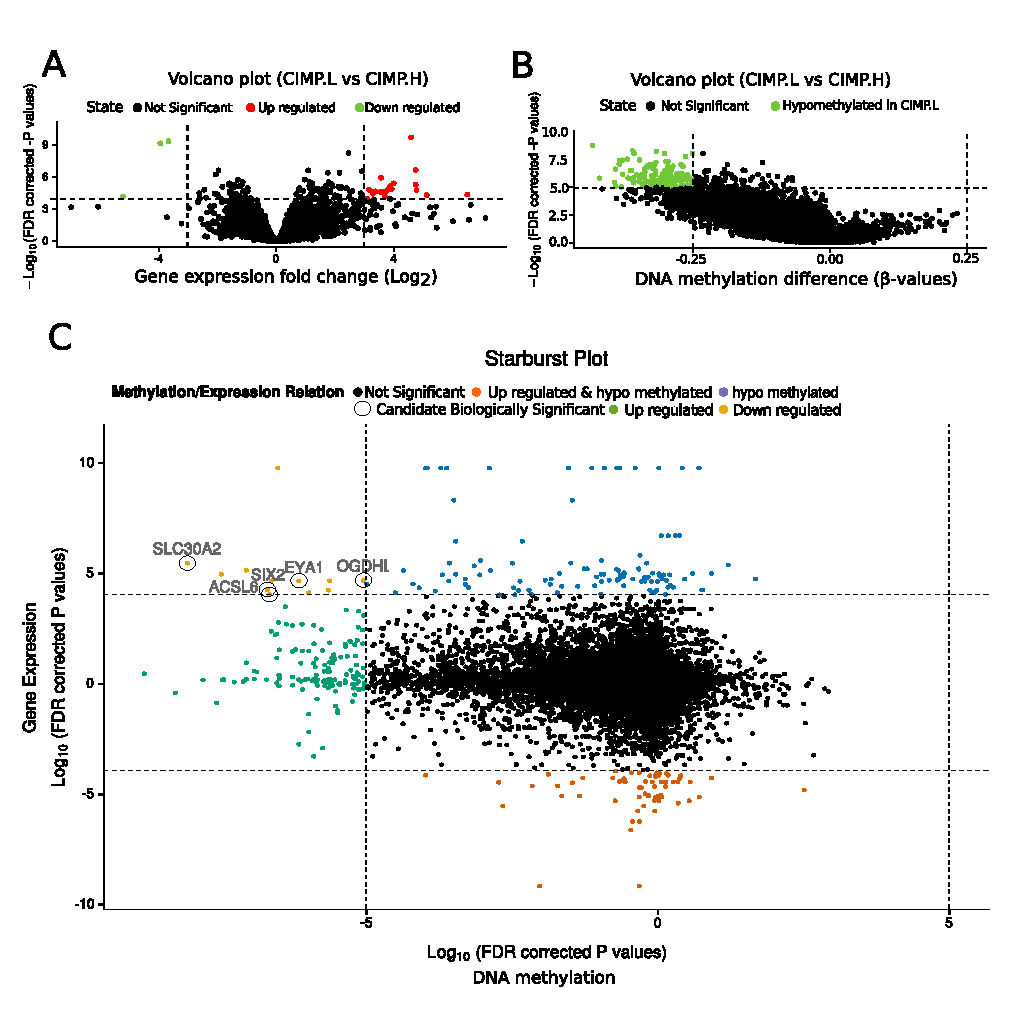
\includegraphics[width=1.0\linewidth]{images/figure5.pdf}
\caption[Case study - Integrative data analysis of Colon Adenocarcinoma]{
Case study - Integrative analysis of gene expression and DNA methylation data from COAD disease,
comparing groups CIMP.L and CIMP.H. \textbf{(A)} Expression volcano plot: fold change of expression data versus significance.
 \textbf{(B)} DNA methylation volcano plot: difference of DNA methylation versus significance.
 \textbf{(C)} Starburst plot: DNA methylation significance versus gene expression significance.}
\label{fig:case_starburst}
\end{figure*}


\section{Use cases using ELMER}\label{sec:analysis_elmer}

%\newpage
\subsection{Breast Invasive Carcinoma (unsupervised approach)} % Optional - only if NO new datasets are included

In this subsection, we describe how to perform \textit{ELMER} analysis on TCGA BRCA
(Breast Invasive Carcinoma) data retrieved from the GDC server.
We first describe how the data can be downloaded and organized to
the default \textit{ELMER} input, followed by the following analysis steps:
\begin{itemize}
	\item Identification of distal probes with significant differential DNA methylation (i.e. DMCs) in tumor vs. normal samples
	\item Identification of putative target gene(s) for differentially methylated distal probes
  \item Characterization of chromatin state context of significant probe regions using FunciVar
	\item Identification of enriched motifs within set of probes in significant probe-gene pairs
	\item Identification of master regulator Transcription Factors (TF) for each enriched motif
\end{itemize}

In addition to these standard steps, we also compared the
putative probe-gene pairs to those derived from deep-sequenced ChIA-PET
data from MCF7 cells (as shown in \citeonline{yao2015inferring}).

\subsubsection*{Downloading TCGA data}

The function \textit{getTCGA} uses the   \href{http://bioconductor.org/packages/TCGAbiolinks/}{TCGAbiolinks}
package \cite{colaprico2015tcgabiolinks} to download TCGA data for all samples
for a given disease (such as BLCA, LGG, GBM). Its main arguments are
the \textit{genome}  that if set to "hg19" will download data from GDC legacy archive, and if set
to "hg38" it will download data from the main GDC harmonized data portal.


%\begin{codigo}[language=R, style = mystyle,label = "download",caption = "Step 1: Downloading TCGA data from GDC database"]
%\end{codigo}

If the \textit{getTCGA} function called before was successful it will
 create the following objects and folders:
\begin{verbatim}
--- DATA/BRCA/
  |----------- BRCA_meth_hg38.rda (object with DNA methylation)
  |----------- BRCA_RNA_hg38.rda (object with gene expression)
  |----------- BRCA_clinic.rda   (object with indexed clinical information)
  |----------- Raw/ (folder: contains All raw data from GDC)
\end{verbatim}

\subsubsection*{Selecting distal probes}

The function \textit{get.feature.probe}, shown in Listing \ref{lst:distal},
is used to select HM450K/EPIC probes located away from any TSS (at least $2Kb$ away).
Its main arguments are the genome of reference ("hg38"/"hg19") and DNA methylation
platform ("450K"/"EPIC"). The \textit{feature} argument is used to limit the region of probes; as we want all distal probes, we set it to NULL.
%Later, we will use all distal probes and annotate their chromatin state later with
%MCF-7 annotation tracks from the NIH Roadmap Epigenomics Mapping Consortium \cite{bernstein2010nih}  available at StateHub (\url{http://statehub.org/})\cite{Coetzee127720}.

\lstinputlisting[language=R,basicstyle=\tiny, frame = none, label = {lst:distal},caption = "Selection of probes within biofeatures"]{codes/distal_probes.R}

\subsection*{Organizing data into a MultiAssayExperiment object}
The function \textit{createMAE} is used to organize the gene expression and
 DNA methylation data into a MultiAssayExperiment (MAE) object. Listing \ref{lst:mae}
 shows how to use it with the data created in the previous steps.
  Its main arguments are described below:

\begin{itemize}
\item \textit{exp} : An R object or a path to a file containing a gene expression
    matrix or SummarizedExperiment with gene counts.
\item \textit{met} : An R object or a path to a file containing a DNA methylation
    matrix or SummarizedExperiment with beta values.
\item \textit{met.platform}: DNA methylation platform.
    "EPIC" for Infinium MethylationEPIC or "450K" for
    Infinium HumanMethylation450.
 \item \textit{genome}: The genome of reference ("hg19" or "hg38")
    used to select the correct metadata. Genes genomic ranges will be annotated
    using ENSEMBL database and DNA methylation probes
    using metadata available at \url{http://zwdzwd.github.io/InfiniumAnnotation}.
 \item \textit{linearize.exp}: this step will take the $log_2(gene\; expression + 1)$
    in order to linearize the relationship between
    gene expression and DNA methylation.
 \item \textit{filter.probes}: genomic ranges (i.e. distal
    regions) within which  probes from
    DNA methylation data should be kept.
 \item \textit{met.na.cut}: maximum percentage of empty values (NA) a probe might have to be
    considered in the analysis. The default is 20\% (i.e if 50\% of samples has empty values  for a given
    probe, it will be removed).
 \item \textit{colData}: A matrix  with samples metadata (i.e. clinical data ,
    molecular  subtype information). If argument TCGA is set to \textit{TRUE}
    this matrix will be created automatically. In this case, the \textit{colData}
    argument is optional.
 \item \textit{sampleMap}: A matrix mapping DNA methylation data and gene expression
    data to samples. \textit{ELMER} uses only samples with both data.
    Otherwise,  it will be removed. If argument TCGA is set to \textit{TRUE}
    this matrix will be created automatically. In this case \textit{sampleMap}
    argument is optional.
\end{itemize}

\lstinputlisting[language=R,basicstyle=\tiny, frame = none, label = {lst:mae},caption = "Create MultiAssayExperiment"]{codes/mae.R}

Listing \ref{lst:verifymae} shows information about the object created.
There are 866 samples with both gene expression and DNA methylation data,
and among those 5 are metastatic samples, 778 are Primary Solid Tumor and
83 are Solid Tissue Normal.

\lstinputlisting[language=R,basicstyle=\tiny, frame = none, label = {lst:verifymae},caption = "Verifying MultiAssayExperiment"]{codes/mae_verify.R}


\subsubsection*{Identification of distal probes with significant differential DNA methylation (i.e. DMCs) in tumor vs. normal samples}

The function \textit{get.diff.meth} is  used to identify regions differentially methylation between two groups.
Listing \ref{lst:diffMeth} shows how to use it to select hypomethylated probes in "Primary solid tumor" samples
when compared to "solid tissue normal" samples  ($FDR \leq 0.01$, $\Delta\overline{\beta}\geq 0.3$), using those samples
in the lower quintile ($minSubgroupFrac = 0.2$) of DNA methylation levels for each probe.
Its main arguments are described below:


\begin{itemize}
\item \textit{data} A multiAssayExperiment with DNA methylation and Gene Expression data.
\item  \textit{group.col}	A column defining the groups of the sample. You can view the available columns using: colnames(MultiAssayExperiment::colData(data)).
\item  \textit{group1}	A group from group.col. \textit{ELMER} will run group1 vs group2. That means, if the direction is hyper, get probes hypermethylated in group 1 compared to group 2.
\item  \textit{group2}	A group from group.col. \textit{ELMER} will run group1 vs group2. That means, if the direction is hyper, get probes hypermethylated in group 1 compared to group 2.
\item \textit{diff.dir} Differential methylation direction. It can be "hypo" which is only selecting hypomethylated probes in group 1 when compared to group 2; "hyper" which is only selecting hypermethylated probes;
\item  \textit{minSubgroupFrac} A number ranging from 0 to 1, specifying the fraction of extreme samples from group 1 and group 2 that are used to identify the differential DNA methylation. The default is 0.2 because we typically want to be able to detect a specific (possibly unknown) molecular subtype among tumor; these subtypes often make up only a minority of samples, and 20\% was chosen as a lower bound for the purposes of statistical power. If you are using pre-defined group labels, such as treated replicates vs. untreated replicated, use a value of 1.0 (\textit{Supervised} mode)

\item  \textit{pvalue} A number specifying the significant P value (adjusted P value by Benjamini-Hochberg procedure) cutoff for selecting significant hypo/hyper-methylated probes. The default is 0.01.
\item  \textit{sig.dif} A number specifying the smallest DNA methylation difference as a cutoff for selecting significant hypo/hyper-methylated probes. The default is 0.3.
\end{itemize}

%\begin{minipage}{\linewidth}
\lstinputlisting[language=R,basicstyle=\tiny, frame = none, label = {lst:diffMeth},caption = "Identify significantly different DNA methylation probes in tumor and normal samples"]{codes/diffMeth.R}
%\end{minipage}

If the \textit{save} argument is set to TRUE, in the \textit{dir.out} folder two files will be created: \textit{getMethdiff.hypo.probes.csv} containing all probes from the DNA methylation data with the difference means of the groups and the significance values, \textit{getMethdiff.hypo.probes.significant.csv} will contain only probes that respect the thresholds. Table \ref{tab:diff.meth} shows the first rows of  \textit{getMethdiff.hypo.probes.significant.csv} file.

\begin{table}[h!]
\csvautobooktabular[respect underscore,
                    filter expr={test{\ifnumless{\thecsvinputline}{5}}}]{tables/getMethdiff.hypo.probes.significant.csv}
\caption[Identification of distal probes with significant differential DNA methylation (i.e. DMCs)]{Identification of distal probes with significant differential DNA methylation (i.e. DMCs): First three rows of  getMethdiff.hypo.probes.significant.csv file. }
\label{tab:diff.meth}
\end{table}

\newpage
\subsubsection*{Identification of putative target gene(s) for differentially methylated distal probes}
The function \textit{get.pair} is used to link enhancer probes with methylation changes to target genes with expression changes and report the putative target gene for selected probes. Listing \ref{lst:getpair} shows how to select the 20 nearest genes (10 downstream and 10 upstream) and evaluate if each pair is anti-correlated (probes with higher methylation levels have lower gene expression levels).
Its main arguments are described below:

\begin{itemize}
\item \textit{nearGenes:} Output of \textit{GetNearGenes} function.
\item  \textit{mode:} Algorithm mode: "unsupervised" or "supervised". If unsupervised is set
the $U$ (unmethylated) and $M$ (methylated) groups will be selected
among all samples of both groups based on methylation of each probe.
Otherwise $U$ group and $M$ group will set as all the samples of group1 or group2 as described below:
If diff.dir is "hypo, $U$ will be the group 1 and $M$ the group2.
If diff.dir is "hyper" $M$ group will be the group1 and $U$ the group2.
\item \textit{minSubgroupFrac:} A number ranging from 0 to 1, specifying the fraction of extreme  samples that define group U (unmethylated) and group M (methylated), which are used to link probes to genes. The default is 0.4 (the lowest quintile of samples is the U group and the highest quintile samples is the M group) because we typically want to be able to detect a specific (possibly unknown) molecular subtype among tumor; these subtypes often make up only a minority of samples, and 20\% was chosen as a lower bound for the purposes of statistical power. This argument is Only used if mode is "supervised", otherwise if you are using pre-defined group labels ("supervised" mode), such as treated replicates vs. untreated replicated, it will use all samples.
\item  \textit{permu.size:} Number of permutation. The default is $10000$. \textit{Note}: This parameter can strongly impact run time.
\item \textit{raw.pvalue:} Raw p-value cutoff for defining significant pairs. The default is $0.001$.
\item \textit{Pe:} Empirical p-value cutoff for defining significant pairs. The default is $0.001$.
\item \textit{filter.probes:} Should probes be filtered  by selecting only those which have at least a certain number of samples below and above a certain cut-off ? If true, arguments \textit{filter.probes} and \textit{filter.percentage} will be used.
\item  \textit{filter.portion:}	A number specifying the cut point to define binary methylation level for probe loci. The default is 0.3. When the beta value is above 0.3, the probe is methylated and vice versa. For one probe, the percentage of methylated and unmethylated samples should be above filter.percentage value. Only used if \textit{filter.probes} is TRUE.
\item  \textit{filter.percentage:}	Minimum percentage of samples to be considered in methylated and unmethylated for the filter.portion option. Default 5\%. Only used if \textit{filter.probes} is TRUE.
\end{itemize}


\lstinputlisting[language=R,basicstyle=\tiny, frame = none, label = {lst:getpair}, caption = "Identify putative target genes for differentially methylated distal probes"]{codes/getpair.R}

The output of this function is shown in table \ref{tab:get.pair}. Probe and GeneID
columns show the significant pair and the column $P_e$ shows the adjusted p-value.
\begin{table}[h!]
\centering
\small
\csvautobooktabular[respect underscore,
					before reading=\sisetup{round-mode=places,round-precision=2},
                    filter expr={test{\ifnumless{\thecsvinputline}{5}}}]{tables/getPair.hypo.pairs.significant.csv}
\caption [Identification of putative target gene(s) for differentially methylated distal probes]{
Identification of putative target gene(s) for differentially methylated distal probes: First three rows of  getPair.hypo.pairs.significant.csv file.
}
\label{tab:get.pair}
\end{table}

To visualize the relationship between the probe-gene pairs inferred, there are two auxiliary functions in ELMER. The function \textit{schematic.plot}, shown in Listing \ref{lst:plotpair}, which will plot genes and probes in a specified genomic region, highlighting the significant pairs identified by plotting a genomic interactions track and highlight the genes in the pair in red (Figure \ref{fig:pairplot}). Also,  using the function \textit{scatter.plot} (Listing \ref{lst:scatterplot}) it is possible to visualize the correlation between gene expression and DNA methylation levels at probe (Figure \ref{fig:scatterplot}).
 Finally, an overall summary of the DNA  methylation levels and gene expression levels  can be visualized using the auxiliary function \textit{heatmapPairs}, as shown in Listing \ref{lst:heatmap}. This function creates a heatmap for all samples  as shown in Figure \ref{fig:heatmap}.

%\begin{minipage}{\linewidth}
\lstinputlisting[language=R,basicstyle=\tiny, frame = none,firstline=5,lastline=13,label = {lst:plotpair},caption = "Schematic plot to visualize gene-probe pairs"]{codes/plotpair.R}
%\end{minipage}

\begin{figure}
\centering
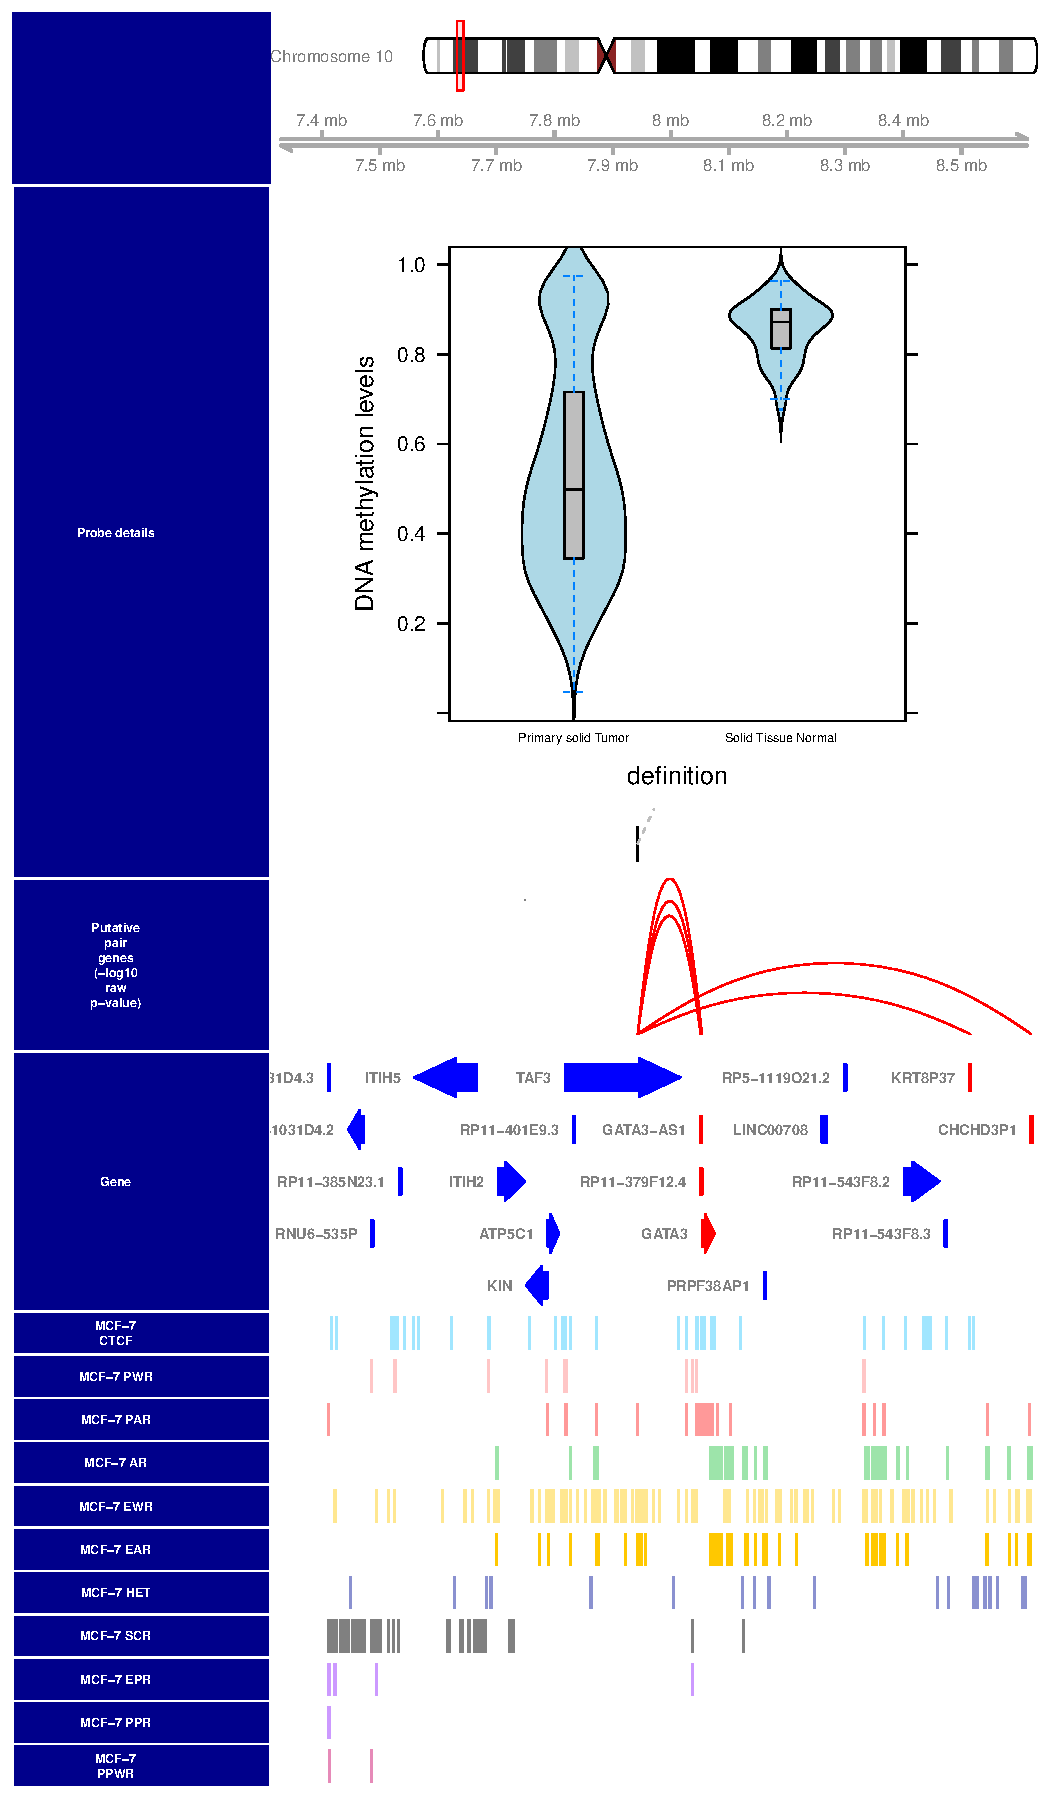
\includegraphics[width=0.7\textwidth]{images/cg04723436_schematic_byProbe.pdf}
\caption[Schematic plot gene-probe pairs]{\label{fig:pairplot} Plot probe-gene pairs with annotation track for MCF-7 cell line from \url{StateHub.org}. Significant probes and gene pairs are highlighted in red.}
\end{figure}

\lstinputlisting[language=R,basicstyle=\tiny, frame = none,label = {lst:scatterplot},caption = "Scatterplot to visualize correlation between gene expression and DNA methylation levels at probe"]{codes/scatterplot.R}


\begin{figure}
\centering
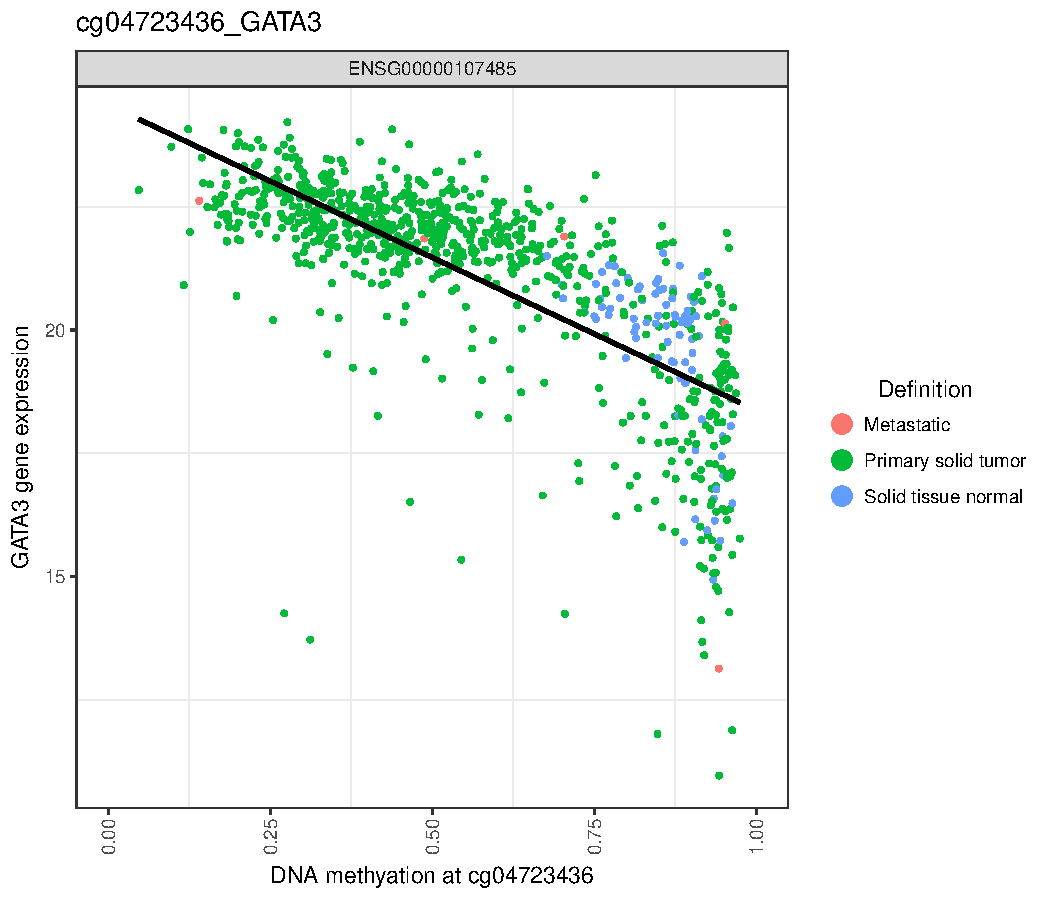
\includegraphics[width=0.7\textwidth]{images/cg04723436_GATA3_bypair.pdf}
\caption{\label{fig:scatterplot} Scatter plot for significant probe (cg04723436) gene (GATA3) pair.}
\end{figure}

\begin{figure}
\centering
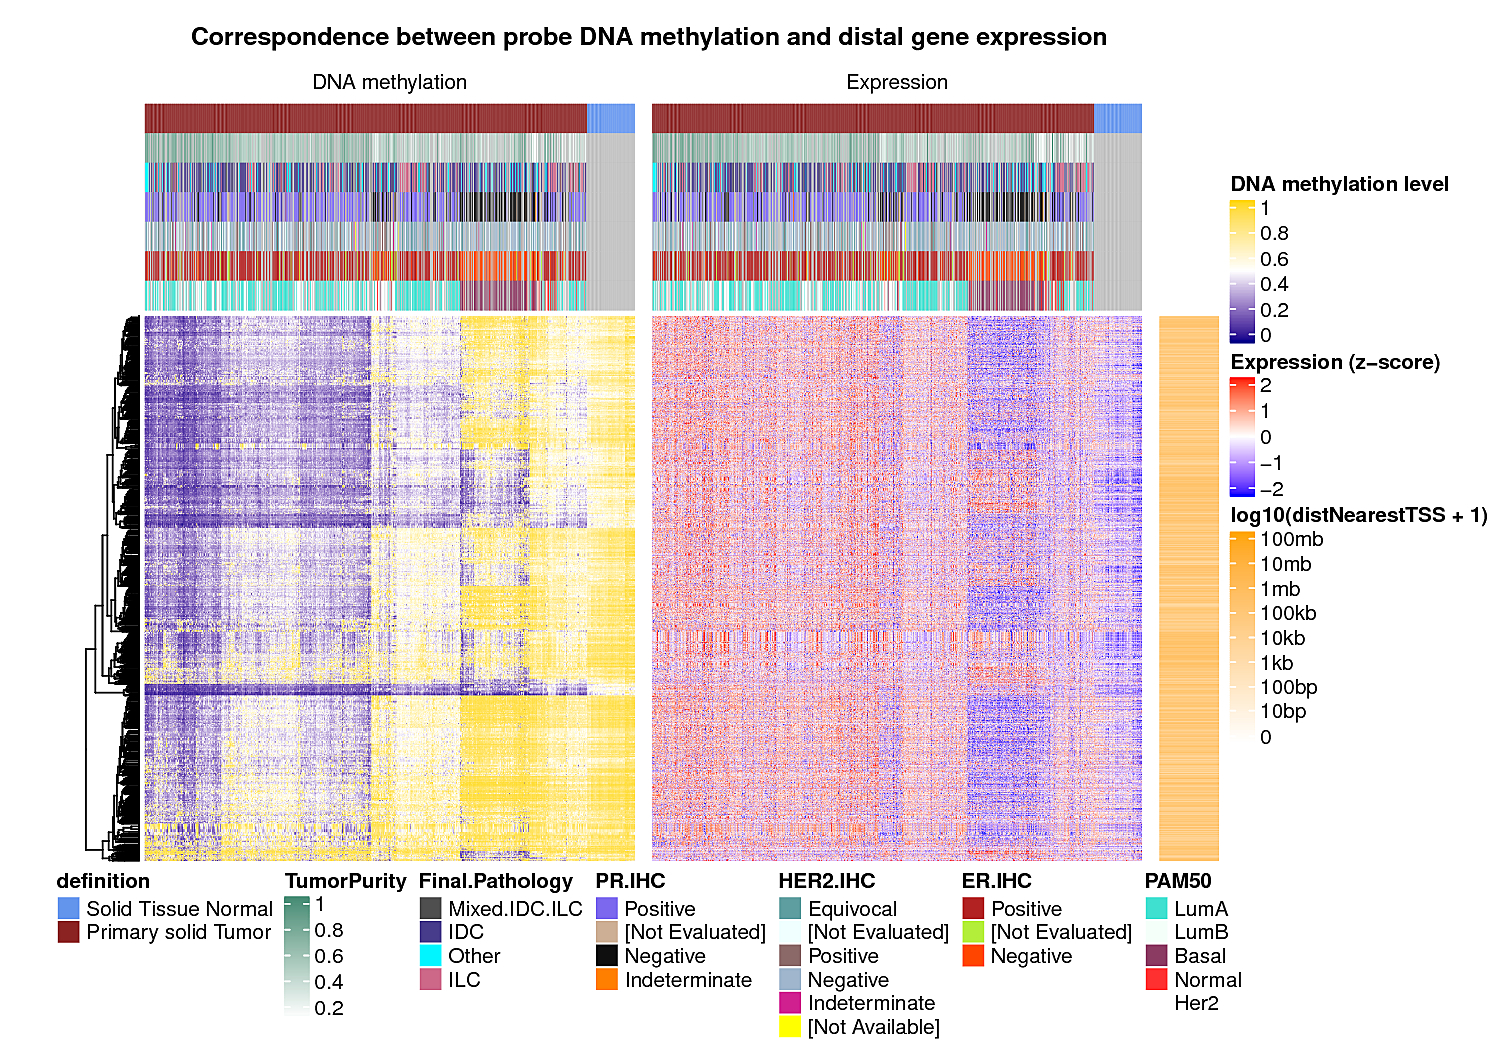
\includegraphics[width=1.0\textwidth]{images/heatmap.jpg}
\caption{\label{fig:heatmap} The comprehensive heatmap view shows all probe / gene pairs identified by ELMER, clustered according to similarity. This plot is based on the Supervised analysis of LumA vs Basal-like Breast Cancer cases. The inverse correlation between methylation and expression can be observed.}
\end{figure}

\clearpage
\lstinputlisting[language=R,basicstyle=\tiny,frame = none,label = {lst:heatmap},caption = "Heatmap to visualize gene-probe pairs"]{codes/heatmap.R}

\clearpage

\subsubsection*{Characterization of chromatin state context of significant probe regions using FunciVar}

To understand and compare our set of probes identified in the probe-gene pairs inferred
we used chromatin state of IHEC cell types
from \url{http://statehub.org/}, to calculate the relative enrichment of
different states.
This procedure uses code from the statepaintR \cite{statepaintr} and FunciVar \cite{funcivar} packages.
Figure \ref{fig:funcivar} shows the enrichment for 14 encode cells lines.
The plot shows enrichment for enhancer active region (EAR), weak enhancer (EWR)
and active promoter region (PAR) in MCF-7 cell (human breast adenocarcinoma cell line)
while for other cell lines this enrichment is not visible.

% https://www.ebi.ac.uk/training/online/course/functional-genomics-introduction-embl-ebi-resource/what-functional-genomics-1
%The functional genomics studies investigates a range of processes such as transcription, translation and epigenetic regulation to understand the complex relationship between genotype and phenotype. Among the main issues it tries to elucidate, we can mention  understanding of the regulation of the genes, finding the active gene promoters in a particular cell type and identifying the functional roles of different genes.
%In view of these questions, several international consortia emerged whose objectives could help clarify some of these issues.
%As examples of these consortia we can cite ENCODE (Encyclopedia of DNA Elements) whose objective was to create a comprehensive catalog of candidate functional elements in the genome and REMC (the Roadmap Epigenomics Mapping Centers project), whose objective was to generate reference epigenomic maps for “normal” human cells/tissues.

%These consortia made available a large amount of data such as transcription, transcription factor binding, histone modifications, DNase hypersensitivity, DNA methylation, DNA-DNA interactions, and RNA-protein interactions that have been used to  annotate chromatin state. Listing shows how to use MCF-7 annotation tracks from \url{http://statehub.org/}  to annotate chromatin state of those pairs identified previously.  (see Additional file for the code

%\begin{minipage}{\linewidth}
%\lstinputlisting[language=R,basicstyle=\tiny, frame = none,basicstyle=\ttfamily\scriptsize]{codes/enhancer.R}
%\end{minipage}
%\begin{minipage}{\linewidth}
%\lstinputlisting[language=R,basicstyle=\tiny, frame = none,basicstyle=\ttfamily\scriptsize,label = {lst:funcivar},caption = "Chromatin state annotation for probe regions"]{codes/funcivar.R}
%\end{minipage}

\begin{figure}
\centering
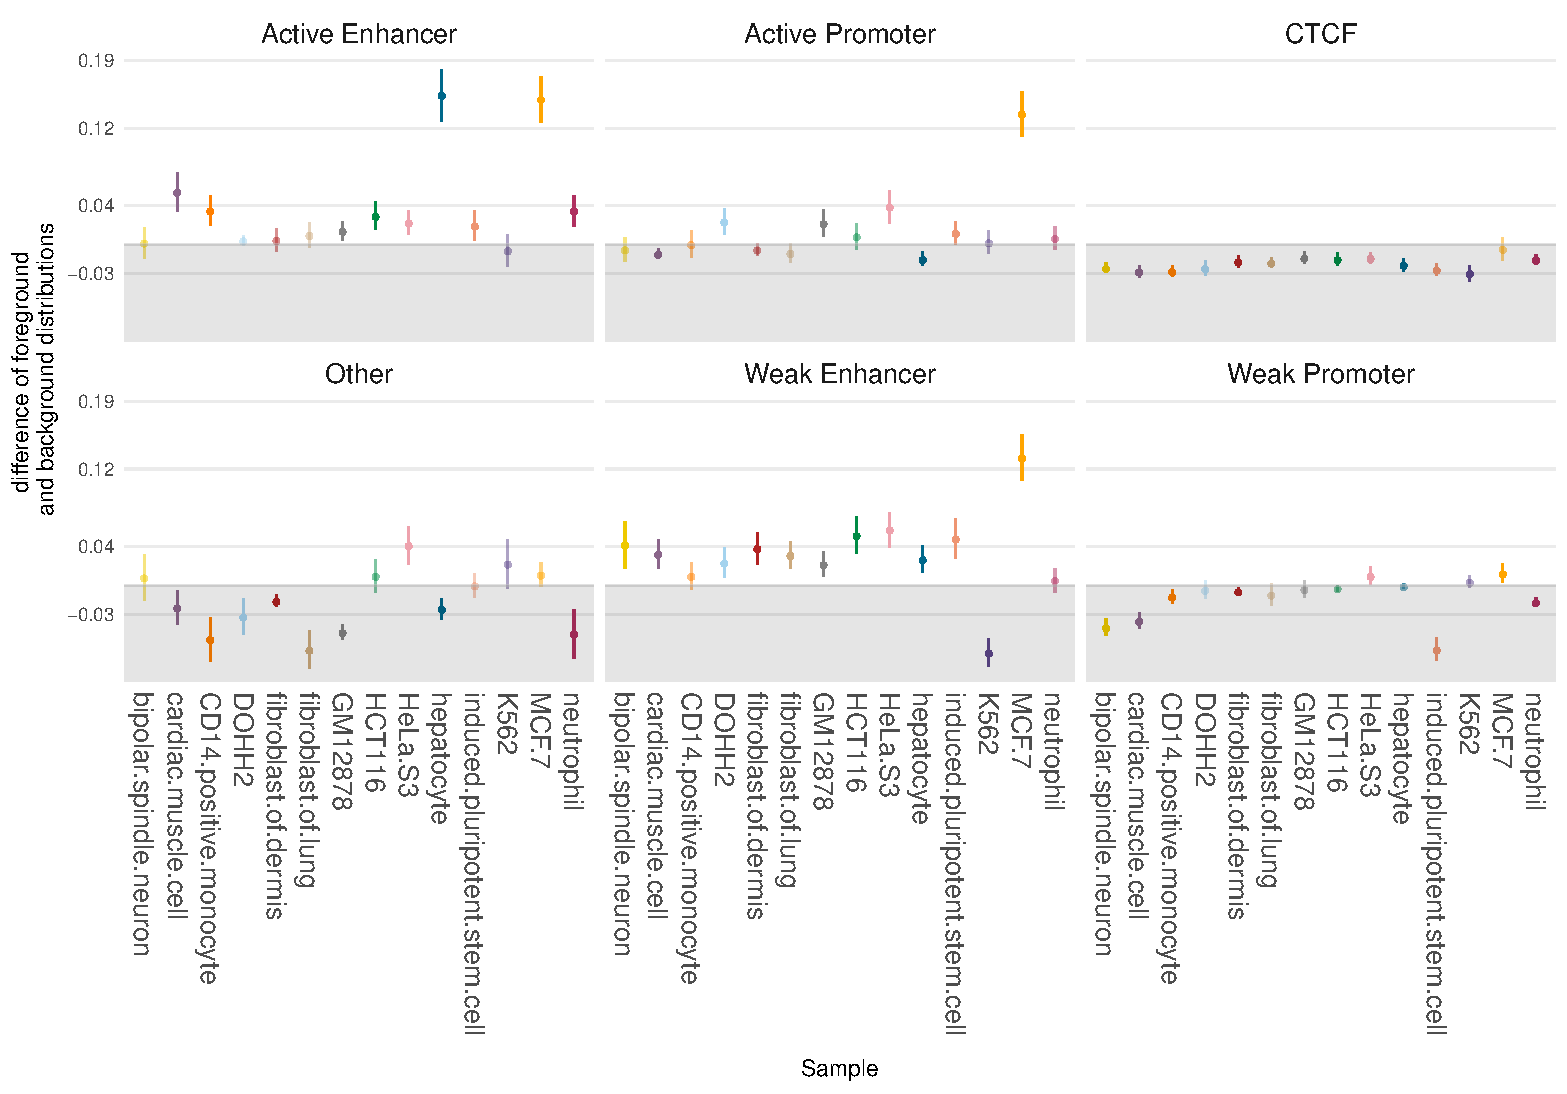
\includegraphics[width=1.0\textwidth]{images/funcivar.pdf}
\caption[ Enrichment of paired probes and chromatin states of encode cells.]{\label{fig:funcivar} Enrichment of paired probes and chromatin states of encode cells.
The plot shows enrichment for enhancer active region, weak enhancer  and active
promoter region for MCF-7 cell. Acronyms - AR: Active region, EAR: active enhancer,
 EWR: Weak Enhancer, EPR: poised enhancer, PAR: active promoter, PWR: Weak Promoter,
 PPR: poised promoter, PPWR: Weak Poised Promoter, CTCF: architectural complex,
 TRS: transcribed, HET: heterochromatin, SCR: Polycomb Repressed Silenced}
\end{figure}


%\cleardoublepage

\subsubsection*{Identification of enriched motifs within set of probes in significant probe-gene pairs}
The function \textit{get.enriched.motif} is used to identify enriched motif in a set of probes.
The main arguments are described below:
\begin{itemize}
\item \textit{lower.OR}	 The motif with lower boundary of 95\% confidence interval for Odds Ratio $\geq lower.OR$  are the significantly enriched motifs.
\item \textit{min.incidence} Minimum number of probes having the motif signature (default: 10) required for a motif to be enriched.
\end{itemize}

%\begin{minipage}{\linewidth}
\lstinputlisting[language=R,basicstyle=\tiny, frame = none,label = "motif",caption = "Motif enrichment analysis on the selected probes"]{codes/motif.R}
%\end{minipage}

\begin{figure}
\centering
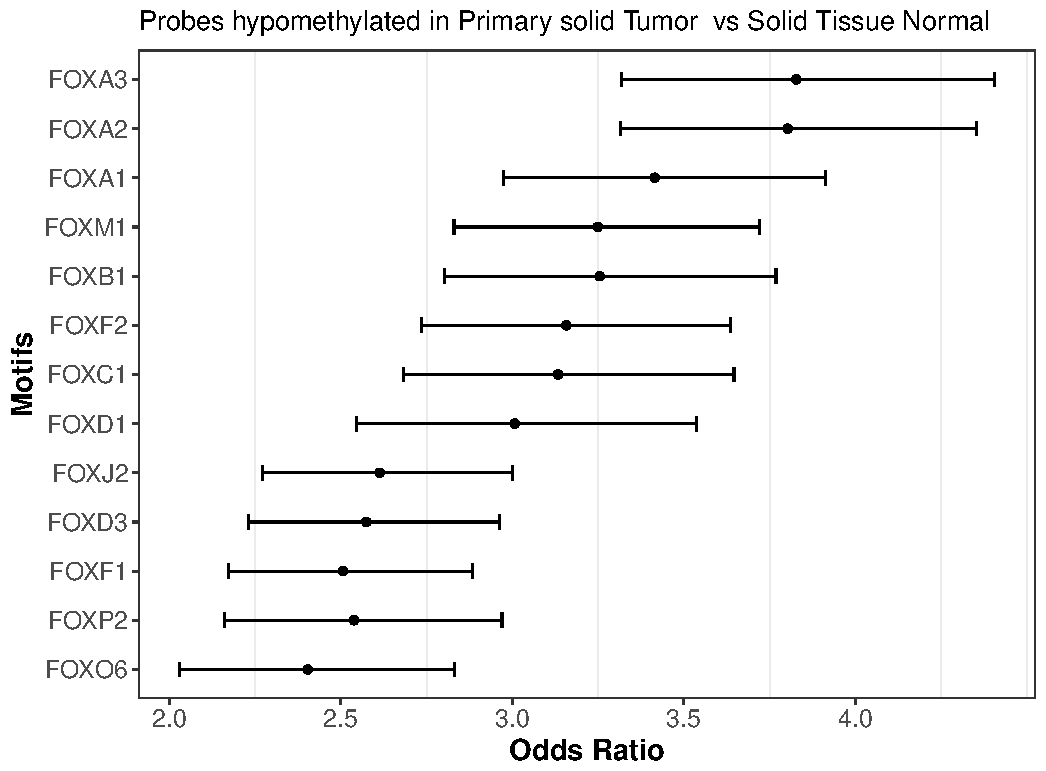
\includegraphics[width=1.0\textwidth]{images/motif_new.pdf}
\caption{\label{fig:motifplot} Motif enrichment plot shows the enrichment levels ($OR\geq2.0$) for the most significant motifs based on the TCGA Breast Cancer Unsupervised analysis. A number of less significant motifs meet our default OR threshold of 1.1 ($\textit{lower.or}=1.1$), which can be browsed in our full Supplemental output report.}
\end{figure}

%\cleardoublepage
\subsubsection*{Identification of master regulator Transcription Factors (TF) for each enriched motif}
The function \textit{get.TFs} is used to identify regulatory TF whose expression associates with TF binding motif
DNA methylation which.

\lstinputlisting[language=R,basicstyle=\tiny, frame = none,label = "tf",caption = "Identifying regulatory Transcript Factors"]{codes/tf.R}

The result of this function is shown in table \ref{tab:get.tf} and in figure \ref{fig:tfplot}.

\begin{landscape}

\begin{table}
\centering
\small
\csvautobooktabular[respect underscore,
					before reading=\sisetup{round-mode=places,round-precision=2},
                    filter expr={test{\ifnumless{\thecsvinputline}{20}}}]{tables/getTF.hypo.significant.TFs.with.motif.summary.csv}
\caption[Identification of master regulator Transcription Factors (TF) for each enriched motif] {First twenty rows of  the \textit{getTF.hypo.significant.TFs.with.motif.summary.csv} file created by \textit{get.Tfs} function (suffix "\_HUMAN.H11MO" was removed from motifs names). First column shows the enriched motif, "top\_5percent\_TFs" shows the top 5\% TFs ranked (the same as all TFs to the left of the dashed line in figure \ref{fig:tfplot}), "potential.TFs.family" are the TF from the "top\_5percent"  that belongs to the same family as the TF of the motif, "top.potential.TFs.family" is the highest ranked TF belonging to the same family as the TF of the motif (same as the first TF from "potential.TFs.family" column). The columns "potential.TFs.subfamily" and "top.potential.TFs.subfamily" are the same as "potential.TFs.family" and "top.potential.TFs.family"  but considering the subfamily classification instead. For example, the motif ANDR has two TFs in the top 5\% that belongs to the same TF family (Steroid hormone receptors): ESR1 and AR, but if considering subfamilies only AR in considered.
}
\label{tab:get.tf}
\end{table}
\end{landscape}


\begin{figure}
\centering
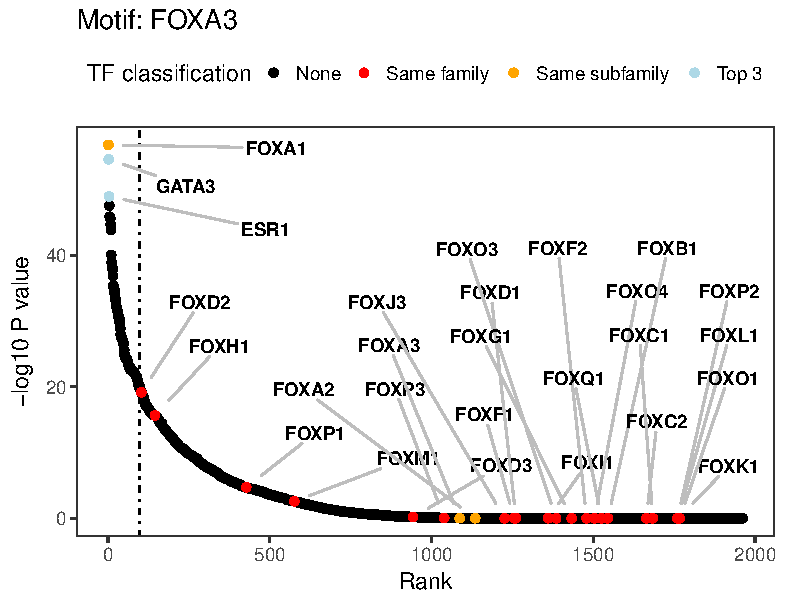
\includegraphics[width=0.9\textwidth]{images/TFranking.pdf}
\caption{\label{fig:tfplot} TF ranking plot shows the statistical $-log_{10}(P-value)$ assessing the anti-correlation level of candidate Master Regulator TF expression with average DNA methylation level for sites with the given motif (FOXA3). By default, the top 3 associated TFs (blue dots), and all of the TF family members (red dots) and subfamily members (orange dots) are labeled. The anti-correlation data for the top three candidates (FOXA1, GATA3, and ESR1) are derived from the data shown in Figure \ref{fig:scatter}}
\end{figure}

\begin{figure}
\centering
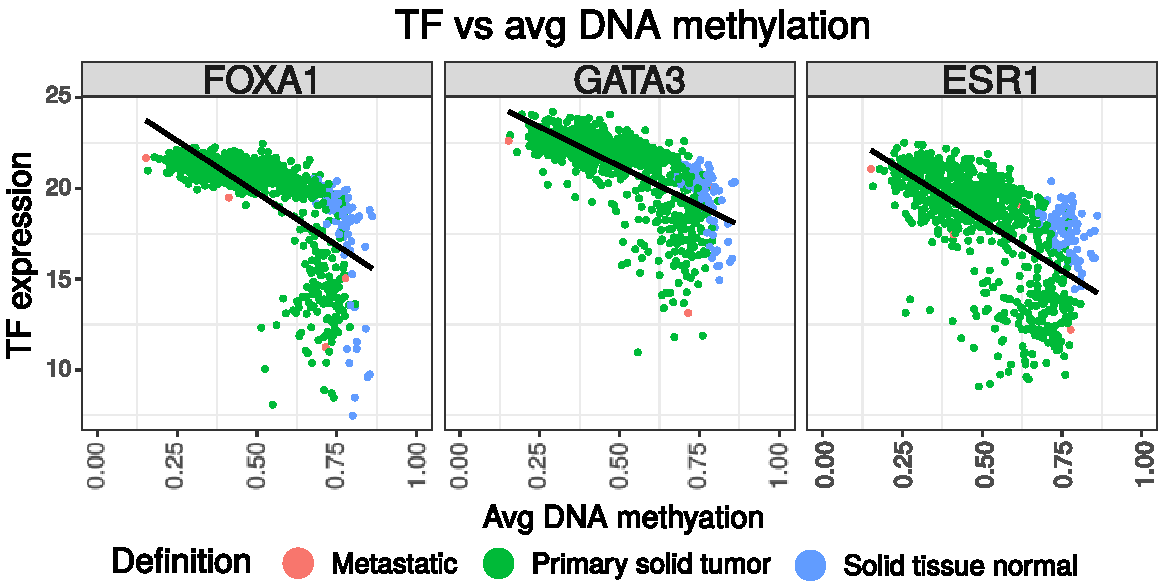
\includegraphics[width=1.0\textwidth]{images/scatter_font.pdf}
\caption{\label{fig:scatter} FOXA1, GATA3 and ESR1 were identified as the most significant Master Regulator candidates for the top motif (FOXA3). All FOX factors belonging to the same TFClass binding family are highlighted.}
\end{figure}

%\clearpage


\subsubsection*{Comparing inferred results with MCF-7 chIA-PET}

As shown in \citeonline{yao2015inferring}, we compared the putative pairs inferred to the chromatin loops derived from deep-sequenced ChIA-PET data from MCF7 cells \cite{li2012extensive}. First, we identify the number of \textit{ELMER} pairs overlapping the ChIA-PET loops, then we repeat using randomly generated  pairs with properties similar to the \textit{ELMER} pairs. For each true ELMER probe in a probe-gene pair, we randomly select a different probe from the complete set of distal probes. We then choose the nth nearest gene to the random probe, where n is the same as the adjacency of the true ELMER probe (i.e. if the true probe is linked to the second gene upstream, the  random probe will also be linked to its second gene upstream). Thus, the random linkage set has both the same number of probes and the same number of linked genes as the true set. One hundred such random datasets were generated to arrive at a 95\% CI ($\pm 1.96* SD$).
The result is shown in Figure \ref{fig:chiapet}. Of the 2124 putative pairs identified in breast cancer tumors, 316 (approximately 14.9\%) were also identified as loops in the MCF7 ChIA-PET data. This was a three-fold enrichment over randomized probe-gene pairs (see Additional file for the code).


\begin{figure}
\centering
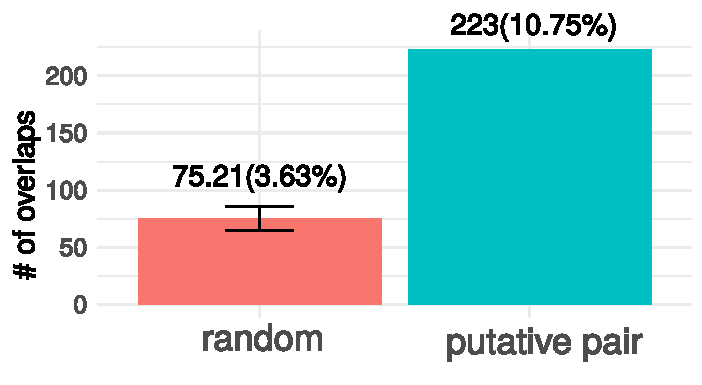
\includegraphics[width=0.5\textwidth]{images/mcf7.pdf}
\caption[MCF7 ChIA-PET validation]{\label{fig:chiapet} The graph shows the comparison of the number of probe-gene pairs identified within MCF7 ChIA-PET data using the putative pairs from BRCA vs. random pairs}
\end{figure}

%\clearpage
\subsection{BRCA molecular subtypes analysis (supervised approach)}


Several studies identified distinct molecular Breast Cancer molecular subtypes including luminal-like (Luminal A and Luminal B) subclasses, which are Estrogen receptor-positive (ER-positive), and the basal-like, ErbB2-positive and normal-like subclasses (ER-negative) \cite{perou2000molecular,yersal2014biological,sorlie2001gene}. We performed \textit{ELMER} analysis comparing known molecular subtypes (Her2, Luminal A, Luminal B and Basal-like) using the TCGA BRCA dataset and classifications retrieved from \cite{ciriello2015comprehensive} using TCGABiolinks.
% TIAGO IS THIS CORRECT?  DID YOU USE BIOLINKS? 
% Yes, the data was downloaded using TCGAbiolionks 
% The annotation was added manually

We performed pairwise analyses between different molecular subtypes. It is important to note that we expect these analyses to have increased statistical power over Unsupervised analyses, as illustrated above in Figure \ref{fig:mode}. One useful output plot is the comprehensive heatmap, 
which illustrates the identification of inverse correlated probe-gene pairs \ref{fig:heatmap} for the LumA vs Basal-like analysis.  

\begin{figure}[ht!]
\centering
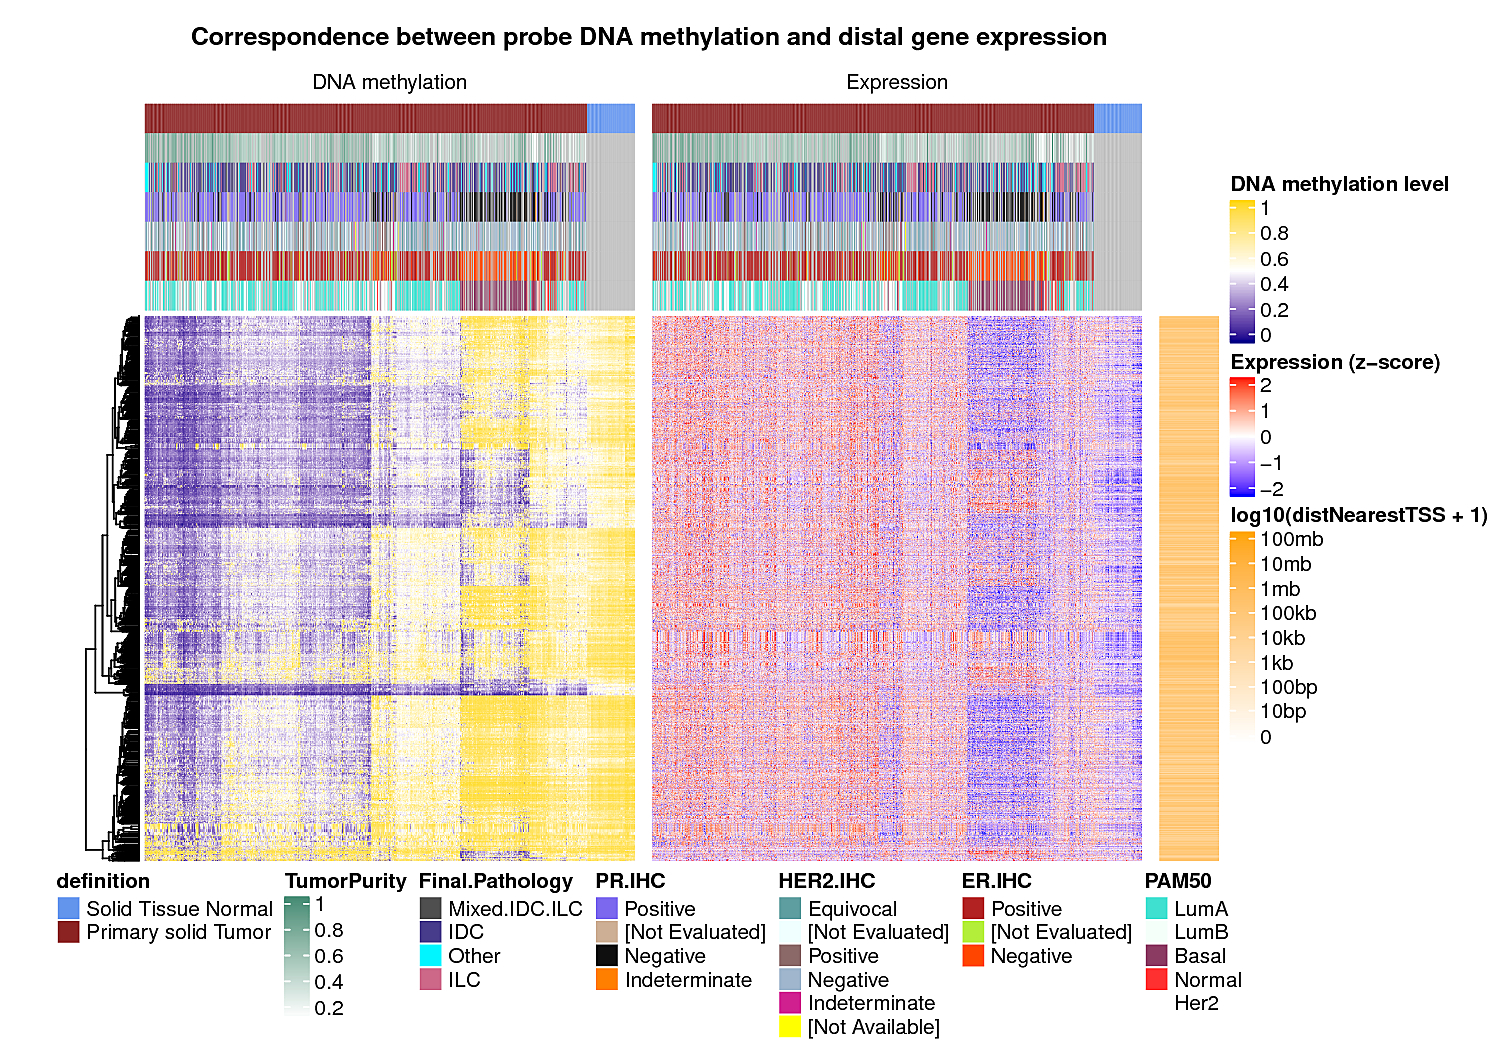
\includegraphics[width=1.0\textwidth]{images/heatmap.jpg}
\caption{\label{fig:heatmap} The comprehensive heatmap view shows all probe / gene pairs identified by ELMER, clustered according to similarity. This plot is based on the Supervised analysis of LumA vs Basal-like Breast Cancer cases. The inverse correlation between methylation and expression can be observed.}
\end{figure}

The unsupervised analysis of the same sample identified several Luminal type Master Regulators (MRs) such as FOXA1, GATA3, and ESR1. In order to identify MRs for the other subtypes, we created a table of candidate MRs identified by each pairwise ELMER run \ref{tbl:TF_molecular} (complete results can be found in the supplemental HTML file described in the Supplementary Methods section). 

Interestingly, several new MRs are identified for the Basal-like group, and these were mostly consistent in comparisons against Luminal and HER2+ subtypes. One group of MRs identified are the \textit{SOX10} and \textit{SOX9} TF signatures. For these signatures, the regulatory TF candidate identified are the \textit{SOX9} (Sry-related HMG box-9) TF and \textit{SOX11} (Sry-related HMG box-11) TF; this correlation between basal-like and SOX11 was recently described by \cite{shepherd2016sox11} and \textit{SOX9} was described by \cite{gong2015foxa1}. Most interestingly, we found KLF5 to be a consistently predicted MR for the Basal-like breast subtype. KLF5 is a master pluripotency factor of embryonic stem cells, and has been associated with a number of different cancers. In breast cancer, it's overexpression has been linked to aggressive, ER-negative and basal-like breast cancers \cite{ben2008embryonic}. % PUBMED ID 18443585

\begin{table}[]
\centering
{\small
\caption{Use case 2 - BRCA supervised analysis: Candidate master regulator TFs (MRs) for each molecular subtype found in a pairwise comparison. This table only includes MRs occurring in multiple pairwise comparisons. For the complete table, please see Supplemental Table \ref{suptbl:TF_molecular} in the supplemental material.}
\label{tbl:TF_molecular}
\begin{tabular}{@{}|c|c|c|c|c|c|c|c|c|@{}}
\midrule
\textit{\textbf{TF}} & \textbf{\begin{tabular}[c]{@{}c@{}}LUMA \\ (vs basal)\end{tabular}} & \textbf{\begin{tabular}[c]{@{}c@{}}LUMB \\ (vs basal)\end{tabular}} & \textbf{\begin{tabular}[c]{@{}c@{}}Basal \\ (vs LumB)\end{tabular}} & \textbf{\begin{tabular}[c]{@{}c@{}}Basal \\ (vs HER2)\end{tabular}} & \textbf{\begin{tabular}[c]{@{}c@{}}HER2 \\ (vs Basal)\end{tabular}} \\ \midrule 
\textit{\textbf{AR}} & x & x &  &  &  \\
\textit{\textbf{BCL11A}} &  &  & x & x &  \\
\textit{\textbf{CEBPB}} &  &  & x & x &  \\
\textit{\textbf{E2F3}} &  &  & x & x &  \\
\textit{\textbf{EMX1}} & x & x &  &  &  \\
\textit{\textbf{ESR1}} & x & x &  &  &  \\
\textit{\textbf{ETV6}} &  &  & x & x &  \\
\textit{\textbf{FOXA1}} & x & x &  &  & x \\
\textit{\textbf{FOXP1}} & x & x &  &  & x \\
\textit{\textbf{GATA3}} & x & x &  &  & x \\
\textit{\textbf{GLI1}} & x & x &  &  &  \\
\textit{\textbf{HOXB1}} & x & x &  &  &  \\
%\textit{\textbf{HOXB2}} & x & x &  &  & x \\
\textit{\textbf{HOXB3}} &  &  &  &  & x \\
%\textit{\textbf{HOXB6}} &  &  &  &  & x \\
\textit{\textbf{HOXC10}} &  &  &  &  & x \\
%\textit{\textbf{HOXC11}} &  &  &  &  & x \\
\textit{\textbf{KLF5}} &  &  & x & x &  \\
\textit{\textbf{LMX1B}} & x & x &  &  &  \\
\textit{\textbf{NR2E3}} & x & x &  &  &  \\
%\textit{\textbf{PATZ1}} &  & x &  &  &  \\
\textit{\textbf{PBX1}} &  & x &  &  &  \\
\textit{\textbf{RARA}} & x & x &  &  &  \\
%\textit{\textbf{RUNX3}} &  &  & x &  &  \\
\textit{\textbf{SOX8}} &  &  & x & x &  \\
\textit{\textbf{SOX9}} &  &  & x & x &  \\
\textit{\textbf{SOX11}} &  &  & x &  &  \\
\textit{\textbf{ZNF467}} & x & x &  &  &  \\
\textit{\textbf{ZIC1}} &  &  & x & x &  \\  \hline 
\end{tabular}
}
\end{table}



\section{Glioma analysis}

The \sigla{ELMER}{Enhancer Linking by Methylation/Expression Relationship} tool was used to analyze the molecular differences between the newly identified G-CIMP-low subtype of glioma that was associated with significantly worse survival compared to the G-CIMP-high, recently described by Dr. Noushmehr and his lab (\cite{cell}). 
For this analysis, TCGA data from the NCI's Genomic Data Commons (\sigla{GDC}{Genomic Data Commons}) was downloaded using our R/Bioconductor TCGAbiolinks package. Table \ref{gcimp.samples} summarizes the number of samples in each group that have both DNA methylation data for the Illumina HumanMethylation450 platform (HM450) and gene expression data
(RNA-Seq). and table \ref{gcip.elmer.arg} summarizes the main values for the ELMER arguments.

% Please add the following required packages to your document preamble:
% \usepackage{booktabs}
\begin{table}[h!]
\centering
\begin{flushleft}
\caption{G-CIMP-high vs G-CIMP-low analysis: number of samples with both DNA methylation (HM450) and gene 
expression (RNA-seq) data.}
\end{flushleft}

\label{gcimp.samples}
\begin{tabular}{@{}ll@{}}
\toprule
Group       & Number of samples \\ \midrule
G-CIMP-high & 233               \\
G-CIMP-low  & 11               
\end{tabular}
\end{table}
% Please add the following required packages to your document preamble:
% \usepackage{booktabs}
\begin{table}[h!]
\centering
\caption{G-CIMP-high vs G-CIMP-low analysis: ELMER arguments values}
\label{gcip.elmer.arg}
\begin{tabular}{@{}lll@{}}
\toprule
Step                        & Argument                           & Value  \\ \midrule
createMAE           & genome &  hg38   \\
Pairs correlation/TF analysis            & Mode &  Supervised   \\
All                         & minSubgroupFrac                    & 100\%  \\
DNA methylation differences & min mean difference                & 0.3    \\
DNA methylation differences & p-value adj cut-off                & 0.01   \\
Pairs correlation           & \# permutations                    & 10000  \\
Pairs correlation           & raw p-value cut-off                & 0.001 \\
Pairs correlation           & empirical p-values cut-off         & 0.001 \\
Motif enrichment            & minimum \# probes (enriched motif) & 10     \\
Motif enrichment             & lower.OR                           & 1.1    \\ \bottomrule
\end{tabular}
\end{table}

The results are summarized in Figure \ref{tab:or}, which shows the Odds Ratio (x axis) for the enriched motifs, and in Table  \ref{tab:tf}, 
which  shows the candidate regulatory TFs whose expression anti-correlated with the DNA methylation level on the probes of each enriched motifs. From the most anti-correlated ones, ELMER uses the TFClass classification (\cite{doi:10.1093/nar/gku1064}) to identifies which TFs are  known to bind in those motifs. This classification has two levels, family and subfamily, which groups motifs with a similar signature. Depending on the motif, its family classification might have a very similar signature, otherwise, the subfamily classification is the most indicated.    

\begin{center}
\begin{figure}[h!]
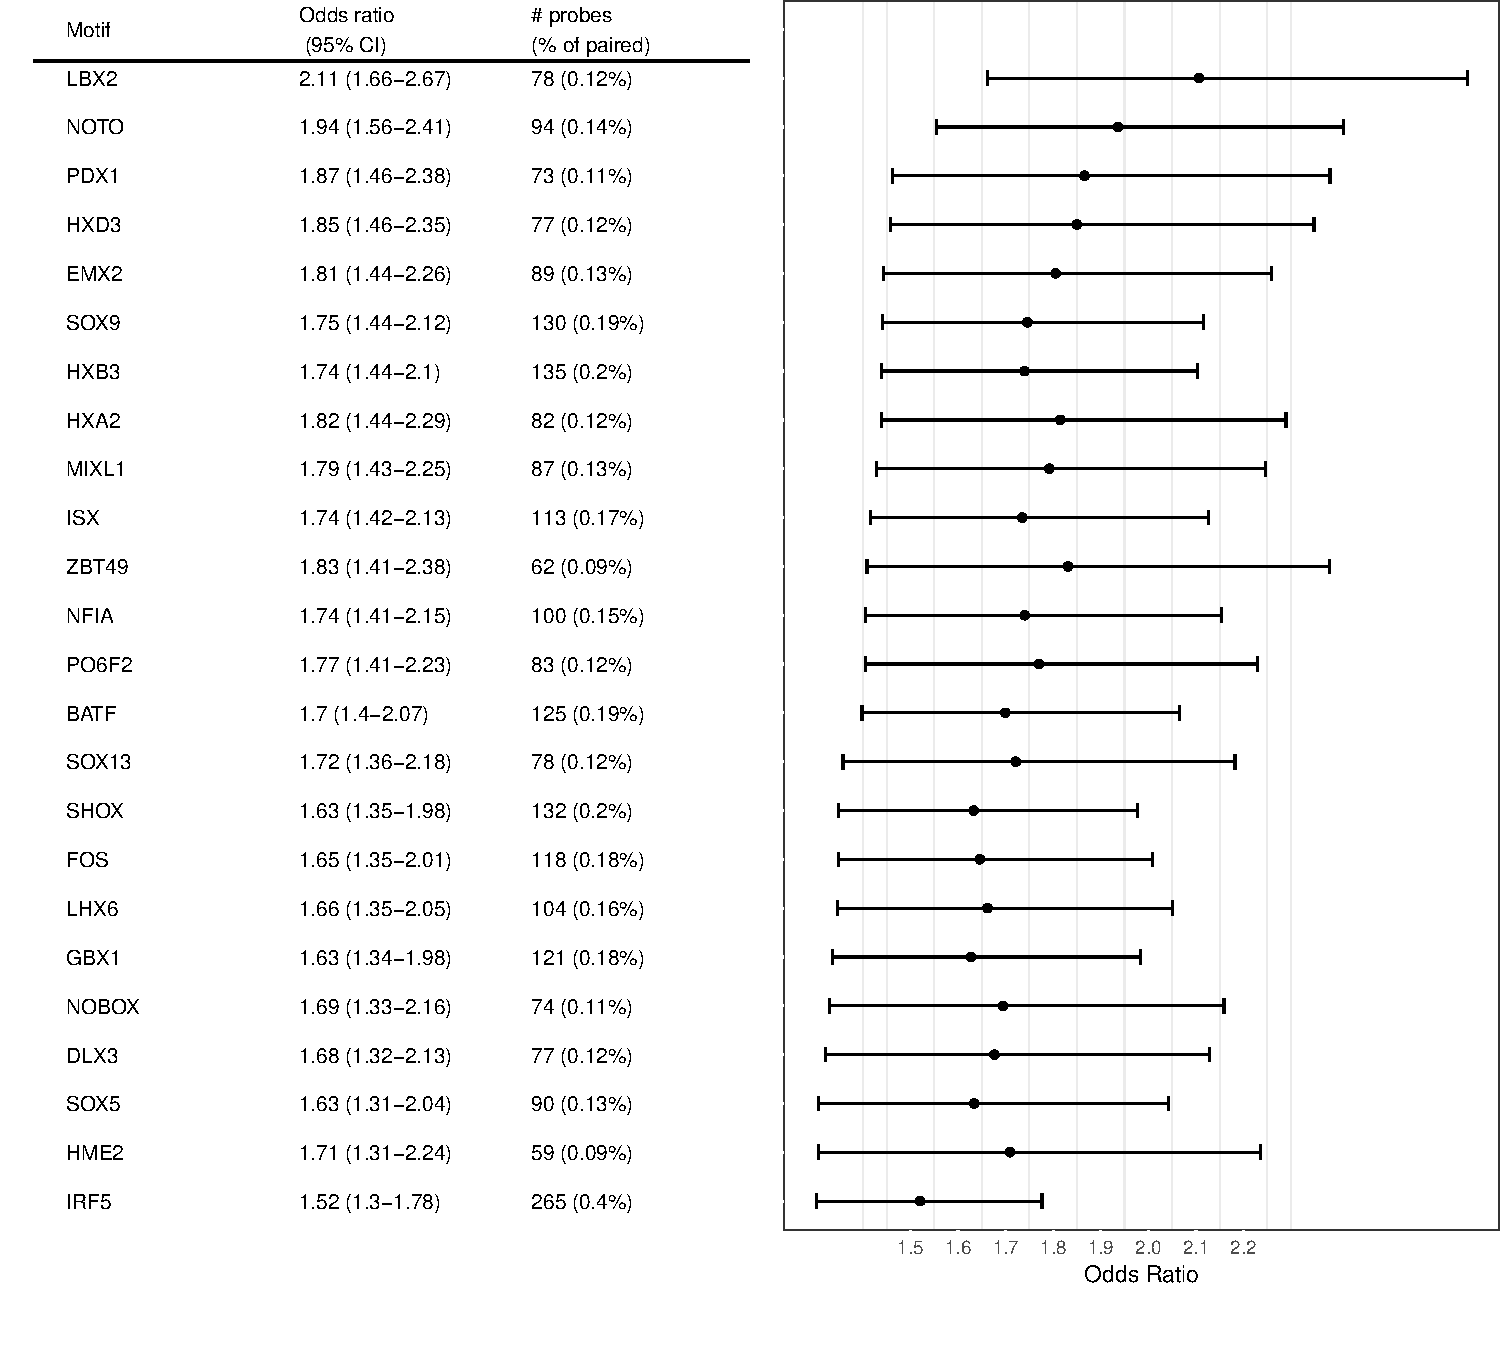
\includegraphics[width=16cm]{images/hyper_motif_enrichment.pdf}
\begin{flushleft}
\captionof{figure}{Motif enrichment analysis: Odds Ratio (x axis) for the selected motifs with OR above 1.5. The range shows the 95\% confidence interval for each Odds Ratio.}
\end{flushleft}
\end{figure}
\label{tab:or}
\end{center}


For example, in Table \ref{tab:tf} the motif HXD3 has as potential TF candidate the HOXD13 if we consider the family \sigla{TF}{Transcription Factor} classification and the HOXD3 TF candidate considering the subfamily TF classification. Figure \ref{tab:hocomoco} shows the motif signature for the HOX-related factors family from \sigla{HOCOMOCO}{HOmo sapiens COmprehensive MOdel COllection} database. The transcription factors \sigla{HOXD13}{Homeobox D13} and \sigla{HOXD3}{Homeobox D3} are in the same family (HOX-related factors) but in different subfamilies.



\begin{table}[h!]
\centering
\caption{TF ranking analysis: statistic For each enriched motif the anti-correlation level of all human TFs expression level with average DNA methylation level at sites with a given motif was access and ranked by the $-log_{10}(P_{value})$, the most relevant one that belongs to the same family as the motif is shown in column \textit{top.potential.TF.family} while the most relevant within the same sub-family classification is shown in column \textit{top.potential.TF.subfamily}}.
\csvautobooktabular[respect underscore]{tables/getTF.hyper.significant.TFs.with.motif.summary.csv}
\label{tab:tf}
\end{table}

\begin{center}
\begin{figure}[h!]
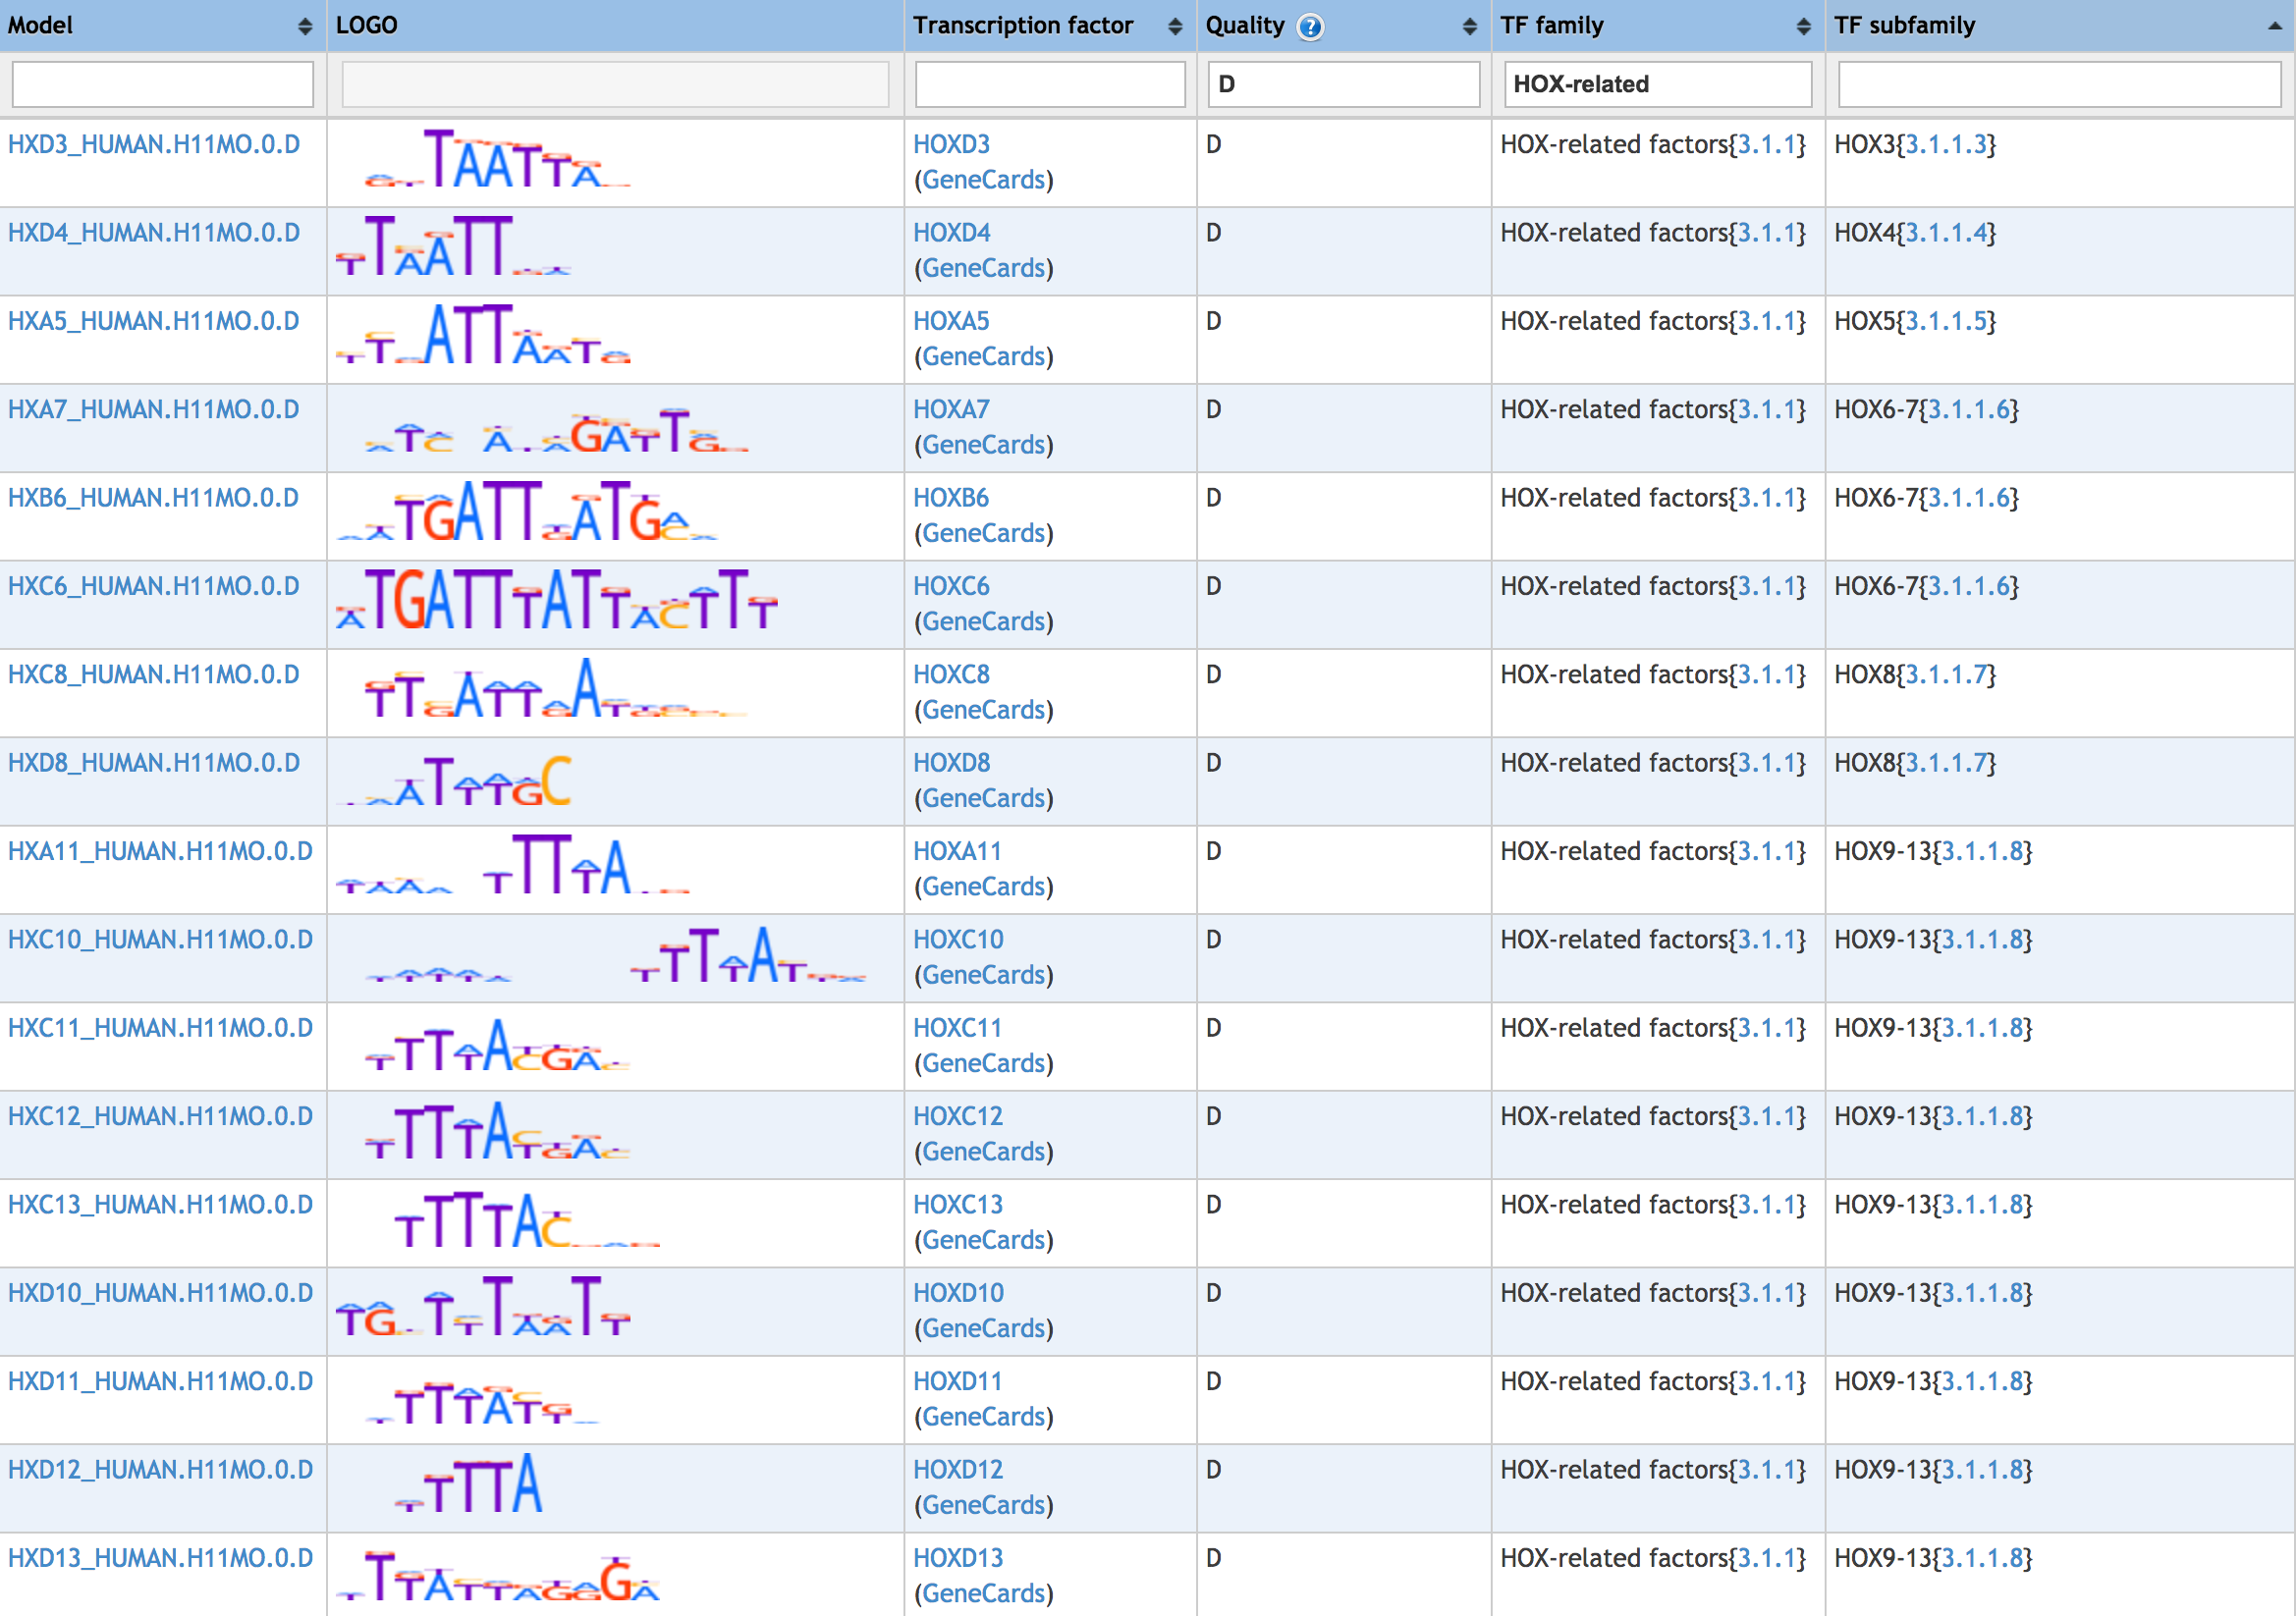
\includegraphics[width=16cm]{images/HOCOMOCO.png}
\caption{HOCOMOCO V11: HOX-related factors family. Transcription factors HOXD13 and HOXD3 are in the same family (HOX-related factors) but in different subfamilies.}
\end{figure}
\label{tab:hocomoco}
\end{center}

To validate those findings, biological experiments are needed which by either knocking down the TF or by regulating the DNA methylation levels of those binding regions will be able to verify if the downstream genes are being regulated.





\chapter{Conclusion}

%\nobibliography{references}

\section{Conclusions}

\section{Publications during the Doctorate Period}
%\nobibliography*{references}
\nobibliography*
As a result of this doctoral project the following articles were published.

\subsection{List of published articles}
\begin{itemize}
	\item \bibentry{10.12688/f1000research.8923.2} 
\end{itemize}

\subsection{List of collaboration articles}
\begin{itemize}
	\item \bibentry{Lingutjnl-2017-314607} 
    \item \bibentry{Malta169680}     
\end{itemize}

\section{Future Works}
%\bibliography{references}



% ---
% Finaliza a parte no bookmark do PDF, para que se inicie o bookmark na raiz
% ---
\bookmarksetup{startatroot}%
% ---

% ----------------------------------------------------------
% ELEMENTOS PÓS-TEXTUAIS
% ----------------------------------------------------------
\postextual

% ----------------------------------------------------------
% Referências bibliográficas
% ----------------------------------------------------------
\bibliographystyle{abntexalfenglish}
\bibliography{thesis}
% ---------------------------------------------------------------------
% GLOSSÁRIO
% ---------------------------------------------------------------------

% Arquivo que contém as definições que vão aparecer no glossário
%\newword{WYSIWYG}{``What You See Is What You Get''  ou ``O que você vê é o que você obtém''.  Recurso tem por objetivo permitir que um documento, enquanto manipulado na tela, tenha a mesma aparência de sua utilização, usualmente sendo considerada final. Isso facilita para o desenvolvedor que pode trabalhar visualizando a aparência do documento sem precisar salvar em vários momentos e abrir em um \textit{software} separado de visualização}
\newword{Framework}{é uma abstração que une códigos comuns entre vários projetos de \textit{software} provendo uma funcionalidade genérica. \textit{Frameworks} são projetados com a intenção de facilitar o desenvolvimento de \textit{software}, habilitando designers e programadores a gastarem mais tempo determinando as exigências do \textit{software} do que com detalhes de baixo nível do sistema}

\newword{Template}{é um documento sem conteúdo, com apenas a apresentação visual (apenas cabeçalhos por exemplo) e instruções sobre onde e qual tipo de conteúdo deve entrar a cada parcela da apresentação}

\newword{Padrões de projeto}{ou \textit{Design Pattern}, descreve uma solução geral reutilizável para um problema recorrente no desenvolvimento de sistemas de \textit{software} orientados a objetos. Não é um código final, é uma descrição ou modelo de como resolver o problema do qual trata, que pode ser usada em muitas situações diferentes}

\newword{Web}{Sinônimo mais conhecido de \textit{World Wide Web} (WWW). É a interface gráfica da Internet que torna os serviços disponíveis totalmente transparentes para o usuário e ainda possibilita a manipulação multimídia da informação}
% Comando para incluir todas as definições do arquivo glossario.tex
\glsaddall
% Impressão do glossário
\printglossaries

% ----------------------------------------------------------
% Apêndices
% ----------------------------------------------------------

% ---
% Inicia os apêndices
% ---
\begin{apendicesenv}

    \chapter{Dispensa comitê de ética}
    \vspace{-2cm}
    \begin{figure}[h!]
    \begin{center}
    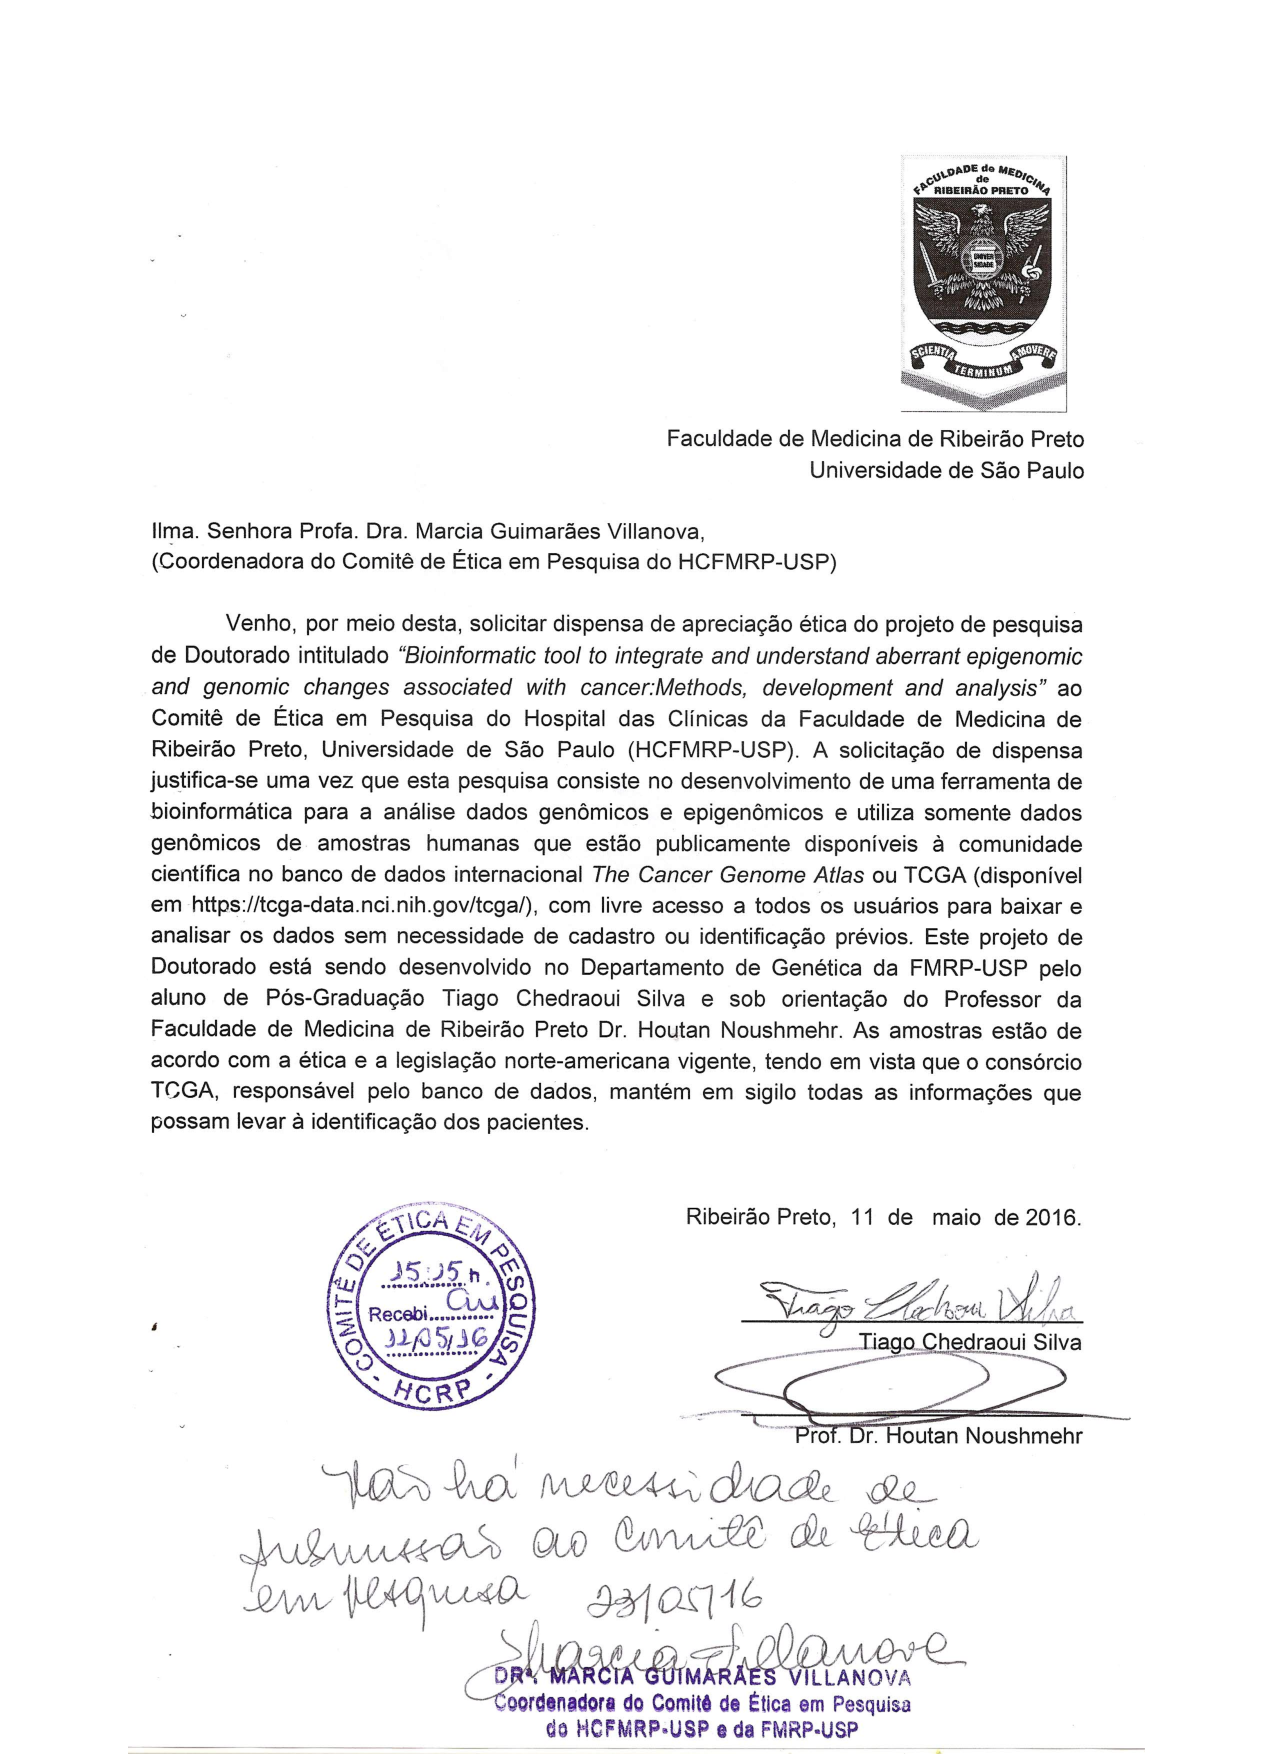
\includegraphics[scale=0.65]{images/dispensa_comite0001.pdf}
    \end{center}
    \end{figure}
%    \label{chapter:documento-basico}
%    \definecolor{gray}{rgb}{0.4,0.4,0.4}
\definecolor{darkblue}{rgb}{0.0,0.0,0.6}
\definecolor{cyan}{rgb}{0.0,0.6,0.6}
\definecolor{maroon}{rgb}{0.5,0,0}
\definecolor{darkgreen}{rgb}{0,0.5,0}


\lstdefinelanguage{myLatex}
{
    keywords={\titulo},
    alsoletter={-},
    sensitive=false,
    morecomment=[l]{\%},
    morecomment=[s]{/*}{*/},
    morestring=[b]",
    morestring=[b]',
    keywordstyle=\bfseries\color{blue},
    commentstyle=\itshape\color{darkgreen},
    morekeywords={documentclass, titulo, autor, data, orientador, coorientador, curso, textoresumo, incluifichacatalografica, textodedicatoria*, textoagradecimentos*, textoepigrafe*, incluilistadefiguras, incluilistadetabelas, incluilistadequadros, incluilistadealgoritmos, incluilistadecodigos, incluilistadesiglas, incluilistadesimbolos, textual, chapter, postextual, begin, bibliography, end}, 
alsoletter={*, \{, \}, \[, \]},
 morekeywords=[2]{\{, \}, \[, \]},
 keywordstyle=[2]\bfseries\color{blue},
 moredelim=[s][\color{maroon}]{\{}{\}},
    moredelim=[s][\itshape\color{maroon}]{\[}{\]},
}

%\lstdefinelanguage{TeX}
%{
%moredelim=*[s][\color{maroon}]{\{}{\}}
%otherkeywords={\{, \}, \[, \], \\}
%  morestring=[b]",
%  moredelim=[s][\bfseries\color{maroon}]{<}{\ },
%  moredelim=[s][\bfseries\color{maroon}]{</}{>},
%  moredelim=[l][\bfseries\color{maroon}]{/>},
%  moredelim=[l][\bfseries\color{maroon}]{>},
%  commentstyle=\color{darkgreen},
%  stringstyle=\color{blue},
%  identifierstyle=\color{red},
%  keywordstyle=\bfseries\color{maroon}
%moredelim=[l][\bfseries\color{maroon}]{>},
%commentstyle=\color{darkgreen},
%  stringstyle=\color{blue},
%  identifierstyle=\color{red}, moredelim=[l][\bfseries\color{maroon}]{\{},
%  keywordstyle=\bfseries\color{maroon}
%}

%\lstset{language={[LaTeX]TeX},
%texcsstyle=*\bfseries\color{blue},
%keywordstyle=\bfseries\color{blue},
%commentstyle=\color{darkgreen},
%morecomment=[s][\color{red}]{\{}{\}},
%otherkeywords={$, \{, \}, \[, \]}
%}

%\begin{codigo}[caption={Exemplo de um documento básico}, label={codigo:documento-basico}, language={[LaTeX]TeX},  breaklines=true,morekeywords={titulo, autor, data, orientador, coorientador, curso, textoresumo, incluifichacatalografica, textodedicatoria*, textoagradecimentos*, textoepigrafe*, incluilistadefiguras, incluilistadetabelas, incluilistadequadros, incluilistadealgoritmos, incluilistadecodigos, incluilistadesiglas, incluilistadesimbolos, {\backslash}textual, chapter, postextual}, alsoletter={{\backslash},*},morecomment=[s][\color{red}]{\{}{\}}]
\begin{codigo}[caption={Exemplo de um documento básico}, label={codigo:documento-basico}, language={myLatex},  breaklines=true]
% Documento utilizando a classe icmc
% Opções: 
%   Qualificação         = qualificacao 
%   Curso                = doutorado/mestrado
%   Situação do trabalho = pre-defesa/pos-defesa (exceto para qualificação)
% -- opções do pacote babel --
% Idioma padrão = brazil
	%spanish,			% idioma adicional para hifenização
	%english,			% idioma adicional para hifenização
	%brazil				% o último idioma é o principal do documento
\ documentclass[doutorado, spanish, english, brazil]{packages/icmc}

% Título do trabalho
\titulo{Título da Monografia}

% Nome do autor
\autor[Abreviação]{Nome completo do autor}

% Data do depósito
\data{18}{12}{2012}

% Nome do Orientador
\orientador[Orientador]{Titulação do orientador}{Nome completo do Orientador}

% Nome do Coorientador (caso não exista basta remover)
\coorientador[Coorientador]{Titulação do coorientador}{Nome completo do Coorientador}
% Se coorientadora troque Coorientador: por Coorientadora dentro do colchetes

% Sigla do programa de Pós-graduação (CCMC, MAT, PIPGES, PROFMAT, MECAI)
\curso{CCMC}
% O valor entre colchetes é opcional para este programa

% Resumo
\textoresumo[Idioma]{
Texto do resumo do trabalho.
}{Lista de palavras-chave separada por virgulas}

% ----------------------------------------------------------
% ELEMENTOS PRÉ-TEXTUAIS
% ----------------------------------------------------------

% Inserir a ficha catalográfica
\incluifichacatalografica{634} % Código Cutter: número atribuído ao sobrenome do autor (disponível em http://www.davignon.qc.ca/cutter1.html).

% Incluí o texto da Dedicatória
\textodedicatoria*{tex/pre-textual/dedicatoria}

% Incluí o texto dos Agradecimentos
\textoagradecimentos*{tex/pre-textual/agradecimentos}

% Incluí o texto da Epígrafe
\textoepigrafe*{tex/pre-textual/epigrafe}

% Inclui a lista de figuras
\incluilistadefiguras

% Inclui a lista de tabelas
\incluilistadetabelas

% Inclui a lista de quadros
\incluilistadequadros

% Inclui a lista de algoritmos
\incluilistadealgoritmos

% Inclui a lista de códigos
\incluilistadecodigos

% Inclui a lista de siglas e abreviaturas
\incluilistadesiglas

% Inclui a lista de símbolos
\incluilistadesimbolos

% Início do documento
\begin{document}

% ----------------------------------------------------------
% ELEMENTOS TEXTUAIS
% ----------------------------------------------------------
\textual

\chapter{Introdução}

Capítulo de Introdução

\chapter{Desenvolvimento}

Capítulo de Desenvolvimento

\chapter{Conclusão}

Capítulo de conclusão

% ----------------------------------------------------------
% ELEMENTOS PÓS-TEXTUAIS
% ----------------------------------------------------------
\postextual

% Nome do arquivo com as referências bibliográficas
\bibliography{referencias}

\end{document}

\end{codigo}

%    \chapter{Configuração do programa JabRef}
%    \label{chapter:configuracao-jabref}
%    \lstdefinelanguage{XML}
{
  morestring=[b]",
  moredelim=[s][\bfseries\color{maroon}]{<}{\ },
  moredelim=[s][\bfseries\color{maroon}]{</}{>},
  moredelim=[l][\bfseries\color{maroon}]{/>},
  moredelim=[l][\bfseries\color{maroon}]{>},
  morecomment=[s]{<?}{?>},
  morecomment=[s]{<!--}{-->},
  commentstyle=\color{darkgreen},
  stringstyle=\color{blue},
  identifierstyle=\color{red}
}


\begin{codigo}[caption={Código de configuração do programa JabRef em XML}, label={codigo:config-jabref}, language=XML, breaklines=true]
<?xml version="1.0" encoding="UTF-8" standalone="no"?>
<!DOCTYPE preferences SYSTEM "http://java.sun.com/dtd/preferences.dtd">
<preferences EXTERNAL_XML_VERSION="1.0">
  <root type="user">
    <map/>
    <node name="net">
      <map/>
      <node name="sf">
        <map/>
        <node name="jabref">
          <map>
            <entry key="KeyPatternRegex" value=""/>
            <entry key="KeyPatternReplacement" value=""/>
            <entry key="abbrAuthorNames" value="true"/>
            <entry key="allowTableEditing" value="false"/>
            <entry key="autoComplete" value="true"/>
            <entry key="autoCompleteFields" value="author;editor;title;journal;publisher;keywords;crossref"/>
            <entry key="autoDoubleBraces" value="true"/>
            <entry key="autoOpenForm" value="true"/>
            <entry key="autoResizeMode" value="4"/>
            <entry key="autoSave" value="true"/>
            <entry key="autoSaveInterval" value="5"/>
            <entry key="autolinkExactKeyOnly" value="true"/>
            <entry key="avoidOverwritingKey" value="false"/>
            <entry key="backup" value="false"/>
            <entry key="caseSensitiveSearch" value="false"/>
            <entry key="citeseerColumn" value="false"/>
            <entry key="confirmDelete" value="true"/>
            <entry key="ctrlClick" value="false"/>
            <entry key="customTypeName_0" value="Article"/>
            <entry key="customTypeName_1" value="Book"/>
            <entry key="customTypeName_10" value="Misc"/>
            <entry key="customTypeName_11" value="Monography"/>
            <entry key="customTypeName_12" value="Patent"/>
            <entry key="customTypeName_13" value="Periodical"/>
            <entry key="customTypeName_14" value="Phdthesis"/>
            <entry key="customTypeName_15" value="Proceedings"/>
            <entry key="customTypeName_16" value="Standard"/>
            <entry key="customTypeName_17" value="Techreport"/>
            <entry key="customTypeName_2" value="Booklet"/>
            <entry key="customTypeName_3" value="Conference"/>
            <entry key="customTypeName_4" value="Electronic"/>
            <entry key="customTypeName_5" value="Inbook"/>
            <entry key="customTypeName_6" value="Incollection"/>
            <entry key="customTypeName_7" value="Inproceedings"/>
            <entry key="customTypeName_8" value="Manual"/>
            <entry key="customTypeName_9" value="Mastersthesis"/>
            <entry key="customTypeOpt_0" value="month;part;section;url;urlaccessdate;note"/>
            <entry key="customTypeOpt_1" value="subtitle;edition;pages;number;series;isbn;volume;org-short;url;urlaccessdate;note"/>
            <entry key="customTypeOpt_10" value="howpublished;month;year;publisher;subtitle;pages;pagename;address;series;number;editortype;url;urlaccessdate;note"/>
            <entry key="customTypeOpt_11" value="pages;pagename;url;urlaccessdate;note"/>
            <entry key="customTypeOpt_12" value="author;title;language;assignee;address;type;number;day;dayfiled;month;monthfiled;url;note"/>
            <entry key="customTypeOpt_13" value="editor;language;series;volume;number;organization;month;url;org-short;note"/>
            <entry key="customTypeOpt_14" value="pages;pagename;url;urlaccessdate;note"/>
            <entry key="customTypeOpt_15" value="editor;volume;number;series;address;publisher;month;organization;org-short;note"/>
            <entry key="customTypeOpt_16" value="author;language;howpublished;type;number;revision;address;month;year;url;org-short;note"/>
            <entry key="customTypeOpt_17" value="pages;pagename;org-short;url;urlaccessdate;number;month;note"/>
            <entry key="customTypeOpt_2" value="subtitle;edition;pages;number;volume;org-short;url;urlaccessdate;note"/>
            <entry key="customTypeOpt_3" value="editor;volume;number;series;pages;address;month;organization;publisher;org-short;note"/>
            <entry key="customTypeOpt_4" value="month;year;org-short;note"/>
            <entry key="customTypeOpt_5" value="booksubtitle;edition;number;series;isbn;volume;org-short;editortype;url;urlaccessdate;note"/>
            <entry key="customTypeOpt_6" value="booksubtitle;edition;number;series;isbn;volume;org-short;editortype;url;urlaccessdate;note"/>
            <entry key="customTypeOpt_7" value="pages;month;publisher;booktitle;conference-location;conference-year;url;urlaccessdate;note"/>
            <entry key="customTypeOpt_8" value="subtitle;author;organization;org-short;address;edition;month;year;pages;series;url;urlaccessdate;note"/>
            <entry key="customTypeOpt_9" value="pages;pagename;url;urlaccessdate;note"/>
            <entry key="customTypeReq_0" value="author;title;journal;year;volume;number;pages"/>
            <entry key="customTypeReq_1" value="title;author/editor/organization;publisher;year;address"/>
            <entry key="customTypeReq_10" value=";author/organization/editor/title"/>
            <entry key="customTypeReq_11" value="author;title;type;school;year;address"/>
            <entry key="customTypeReq_12" value="nationality;number;year;yearfiled"/>
            <entry key="customTypeReq_13" value="title;year"/>
            <entry key="customTypeReq_14" value="author;title;school;year;address"/>
            <entry key="customTypeReq_15" value="title;year"/>
            <entry key="customTypeReq_16" value="title;organization/institution"/>
            <entry key="customTypeReq_17" value="author;title;organization/school;year;address"/>
            <entry key="customTypeReq_2" value="title;author/editor/organization;year"/>
            <entry key="customTypeReq_3" value="author;title;booktitle;year"/>
            <entry key="customTypeReq_4" value="url;urlaccessdate;author/organization/title"/>
            <entry key="customTypeReq_5" value="author;title;editor/organization;booktitle;chapter/pages;publisher;address;year"/>
            <entry key="customTypeReq_6" value="author;title;booktitle;editor/organization;chapter/pages;publisher;address;year"/>
            <entry key="customTypeReq_7" value="author;title;organization;conference-number;year;address"/>
            <entry key="customTypeReq_8" value="title"/>
            <entry key="customTypeReq_9" value="author;title;school;year;address"/>
            <entry key="defaultEncoding" value="ISO8859_15"/>
            <entry key="defaultLabelPattern" value="[auth]:[year]"/>
            <entry key="defaultOwner" value=""/>
            <entry key="defaultShowSource" value="false"/>
            <entry key="dialogWarningForDuplicateKey" value="true"/>
            <entry key="dialogWarningForEmptyKey" value="true"/>
            <entry key="disableOnMultipleSelection" value="false"/>
            <entry key="doNotResolveStringsFor" value="url"/>
            <entry key="enableSourceEditing" value="true"/>
            <entry key="enforceLegalBibtexKey" value="true"/>
            <entry key="exportInOriginalOrder" value="false"/>
            <entry key="exportInStandardOrder" value="true"/>
            <entry key="exportWorkingDirectory" value="/home/marcos/tmp"/>
            <entry key="fileColumn" value="true"/>
            <entry key="fileDirectory" value=""/>
            <entry key="filechooserDisableRename" value="true"/>
            <entry key="floatMarkedEntries" value="true"/>
            <entry key="floatSearch" value="true"/>
            <entry key="fontFamily" value="SansSerif"/>
            <entry key="fontSize" value="12"/>
            <entry key="fontStyle" value="0"/>
            <entry key="generateKeysAfterInspection" value="true"/>
            <entry key="generateKeysBeforeSaving" value="false"/>
            <entry key="gridColor" value="210:210:210"/>
            <entry key="groupAutoHide" value="true"/>
            <entry key="groupAutoShow" value="true"/>
            <entry key="groupExpandTree" value="true"/>
            <entry key="groupKeywordSeparator" value=", "/>
            <entry key="groupShowDynamic" value="true"/>
            <entry key="groupShowIcons" value="true"/>
            <entry key="groupsDefaultField" value="keywords"/>
            <entry key="incompleteEntryBackground" value="250:175:175"/>
            <entry key="incrementS" value="false"/>
            <entry key="lastEdited" value="/home/marcos/Documentos/IFMG/Acadêmico/Aulas/Latex/ifmgbitex/referencias.bib"/>
            <entry key="lastUsedExport" value="html"/>
            <entry key="lookAndFeel" value="com.jgoodies.plaf.plastic.Plastic3DLookAndFeel"/>
            <entry key="markImportedEntries" value="true"/>
            <entry key="markedEntryBackground" value="255:255:180"/>
            <entry key="memoryStickMode" value="false"/>
            <entry key="namesAsIs" value="false"/>
            <entry key="namesFf" value="false"/>
            <entry key="namesLastOnly" value="false"/>
            <entry key="namesNatbib" value="true"/>
            <entry key="openLastEdited" value="true"/>
            <entry key="overrideDefaultFonts" value="false"/>
            <entry key="overwriteOwner" value="false"/>
            <entry key="overwriteTimeStamp" value="false"/>
            <entry key="pdfColumn" value="false"/>
            <entry key="pdfDirectory" value=""/>
            <entry key="posX" value="0"/>
            <entry key="posY" value="0"/>
            <entry key="preview0" value="&lt;font face=&quot;arial&quot;&gt;&lt;b&gt;&lt;i&gt;\bibtextype&lt;/i&gt;&lt;a name=&quot;\bibtexkey&quot;&gt;\begin{bibtexkey} (\bibtexkey)&lt;/a&gt;\end{bibtexkey}&lt;/b&gt;&lt;br&gt;__NEWLINE__\begin{author} \format[HTMLChars,AuthorAbbreviator,AuthorAndsReplacer]{\author}&lt;BR&gt;\end{author}__NEWLINE__\begin{editor} \format[HTMLChars,AuthorAbbreviator,AuthorAndsReplacer]{\editor} &lt;i&gt;(\format[IfPlural(Eds.,Ed.)]{\editor})&lt;/i&gt;&lt;BR&gt;\end{editor}__NEWLINE__\begin{title} \format[HTMLChars]{\title} \end{title}&lt;BR&gt;__NEWLINE__\begin{chapter} \format[HTMLChars]{\chapter}&lt;BR&gt;\end{chapter}__NEWLINE__\begin{journal} &lt;em&gt;\format[HTMLChars]{\journal}, &lt;/em&gt;\end{journal}__NEWLINE__\begin{booktitle} &lt;em&gt;\format[HTMLChars]{\booktitle}, &lt;/em&gt;\end{booktitle}__NEWLINE__\begin{school} &lt;em&gt;\format[HTMLChars]{\school}, &lt;/em&gt;\end{school}__NEWLINE__\begin{institution} &lt;em&gt;\format[HTMLChars]{\institution}, &lt;/em&gt;\end{institution}__NEWLINE__\begin{publisher} &lt;em&gt;\format[HTMLChars]{\publisher}, &lt;/em&gt;\end{publisher}__NEWLINE__\begin{year}&lt;b&gt;\year&lt;/b&gt;\end{year}\begin{volume}&lt;i&gt;, \volume&lt;/i&gt;\end{volume}\begin{pages}, \format[FormatPagesForHTML]{\pages} \end{pages}__NEWLINE__\begin{abstract}&lt;BR&gt;&lt;BR&gt;&lt;b&gt;Abstract: &lt;/b&gt; \format[HTMLChars]{\abstract} \end{abstract}__NEWLINE__\begin{review}&lt;BR&gt;&lt;BR&gt;&lt;b&gt;Review: &lt;/b&gt; \format[HTMLChars]{\review} \end{review}&lt;/dd&gt;__NEWLINE__&lt;p&gt;&lt;/p&gt;&lt;/font&gt;"/>
            <entry key="preview1" value="&lt;font face=&quot;arial&quot;&gt;&lt;b&gt;&lt;i&gt;\bibtextype&lt;/i&gt;&lt;a name=&quot;\bibtexkey&quot;&gt;\begin{bibtexkey} (\bibtexkey)&lt;/a&gt;\end{bibtexkey}&lt;/b&gt;&lt;br&gt;__NEWLINE__\begin{author} \format[HTMLChars,AuthorAbbreviator,AuthorAndsReplacer]{\author}&lt;BR&gt;\end{author}__NEWLINE__\begin{editor} \format[HTMLChars,AuthorAbbreviator,AuthorAndsReplacer]{\editor} &lt;i&gt;(\format[IfPlural(Eds.,Ed.)]{\editor})&lt;/i&gt;&lt;BR&gt;\end{editor}__NEWLINE__\begin{title} \format[HTMLChars]{\title} \end{title}&lt;BR&gt;__NEWLINE__\begin{chapter} \format[HTMLChars]{\chapter}&lt;BR&gt;\end{chapter}__NEWLINE__\begin{journal} &lt;em&gt;\format[HTMLChars]{\journal}, &lt;/em&gt;\end{journal}__NEWLINE__\begin{booktitle} &lt;em&gt;\format[HTMLChars]{\booktitle}, &lt;/em&gt;\end{booktitle}__NEWLINE__\begin{school} &lt;em&gt;\format[HTMLChars]{\school}, &lt;/em&gt;\end{school}__NEWLINE__\begin{institution} &lt;em&gt;\format[HTMLChars]{\institution}, &lt;/em&gt;\end{institution}__NEWLINE__\begin{publisher} &lt;em&gt;\format[HTMLChars]{\publisher}, &lt;/em&gt;\end{publisher}__NEWLINE__\begin{year}&lt;b&gt;\year&lt;/b&gt;\end{year}\begin{volume}&lt;i&gt;, \volume&lt;/i&gt;\end{volume}\begin{pages}, \format[FormatPagesForHTML]{\pages} \end{pages}&lt;/dd&gt;__NEWLINE__&lt;p&gt;&lt;/p&gt;&lt;/font&gt;"/>
            <entry key="priDescending" value="false"/>
            <entry key="priSort" value="entrytype"/>
            <entry key="promptBeforeUsingAutosave" value="true"/>
            <entry key="psDirectory" value=""/>
            <entry key="pushToApplication" value="Insert selected citations into LyX/Kile"/>
            <entry key="recentFiles" value="/home/marcos/Documentos/IFMG/Acadêmico/Aulas/Algoritmos/Algoritmos_exercicios_01/referencias.bib;/home/marcos/Documentos/IFMG/TCC e Projetos/ERP Comparativo/referencias.bib"/>
            <entry key="regExpSearch" value="true"/>
            <entry key="rememberWindowLocation" value="true"/>
            <entry key="resolveStringsAllFields" value="false"/>
            <entry key="runAutomaticFileSearch" value="false"/>
            <entry key="saveInOriginalOrder" value="false"/>
            <entry key="saveInStandardOrder" value="true"/>
            <entry key="searchAll" value="false"/>
            <entry key="searchAllBases" value="false"/>
            <entry key="searchGen" value="true"/>
            <entry key="searchOpt" value="true"/>
            <entry key="searchPanelVisible" value="false"/>
            <entry key="searchReq" value="true"/>
            <entry key="secDescending" value="false"/>
            <entry key="secSort" value=""/>
            <entry key="selectS" value="false"/>
            <entry key="showSearchInDialog" value="false"/>
            <entry key="showSource" value="true"/>
            <entry key="sizeX" value="1280"/>
            <entry key="sizeY" value="800"/>
            <entry key="stringsPosX" value="340"/>
            <entry key="stringsPosY" value="200"/>
            <entry key="stringsSizeX" value="600"/>
            <entry key="stringsSizeY" value="400"/>
            <entry key="tableBackground" value="255:255:255"/>
            <entry key="tableColorCodesOn" value="true"/>
            <entry key="tableOptFieldBackground" value="230:255:230"/>
            <entry key="tableReqFieldBackground" value="230:235:255"/>
            <entry key="tableText" value="0:0:0"/>
            <entry key="terDescending" value="false"/>
            <entry key="terSort" value=""/>
            <entry key="timeStampField" value="timestamp"/>
            <entry key="timeStampFormat" value="dd/MM/yyyy"/>
            <entry key="unmarkAllEntriesBeforeImporting" value="true"/>
            <entry key="urlColumn" value="true"/>
            <entry key="useDefaultLookAndFeel" value="true"/>
            <entry key="useIEEEAbrv" value="true"/>
            <entry key="useImportInspectionDialog" value="true"/>
            <entry key="useImportInspectionDialogForSingle" value="true"/>
            <entry key="useNativeFileDialogOnMac" value="false"/>
            <entry key="useOwner" value="false"/>
            <entry key="useRegExpSearch" value="false"/>
            <entry key="useRemoteServer" value="false"/>
            <entry key="useTimeStamp" value="true"/>
            <entry key="useXmpPrivacyFilter" value="false"/>
            <entry key="warnAboutDuplicatesInInspection" value="true"/>
            <entry key="warnBeforeOverwritingKey" value="true"/>
            <entry key="windowMaximised" value="false"/>
            <entry key="workingDirectory" value="/home/marcos/Documentos/IFMG/Acadêmico/Aulas/Algoritmos/Algoritmos_exercicios_01"/>
          </map>
          <node name="labelPattern">
            <map/>
          </node>
        </node>
      </node>
    </node>
  </root>
</preferences>

\end{codigo}

\end{apendicesenv}
% ---


% ----------------------------------------------------------
% Anexos
% ----------------------------------------------------------

% ---
% Inicia os anexos
% ---
\begin{anexosenv}
    %\chapter{Appendix}
    %\label{chapter:paginas-interessantes}

\end{anexosenv}
% ---

\end{document}
